\documentclass[11pt,twoside,a4paper,openright]{report}
%synctex =====EXPERIMENTAL======
\synctex=1

% Select encoding of your inputs
\usepackage[utf8]{inputenc}

% Make latex understand and use the typographic
% rules of the language used in the document.
\usepackage[english]{babel}

% Use the vector font Latin Modern which is going
% to be the default font in latex in the future.
\usepackage{lmodern}

% Choose the font encoding
\usepackage[T1]{fontenc}

% Use color in tables
\usepackage[table]{xcolor}
\usepackage{array}
\usepackage{multirow}

% Load a colour package
\usepackage{xcolor}
\definecolor{aaublue}{RGB}{33,26,82}  %<--define aaublue
\definecolor{white}{RGB}{255,255,255} %<--define white

% The standard graphics inclusion package
\usepackage{graphicx}

\makeatletter
  \g@addto@macro\@floatboxreset\centering %<--centering all figures
\makeatother

\usepackage{adjustbox}

% Set up how figure and table captions are displayed
\usepackage{float}
\usepackage{caption}
\usepackage{subcaption}
\setlength{\belowcaptionskip}{-0.5cm}
\captionsetup
{
  justification = centering,    %<--centering caption with multiple lines
  font          = footnotesize, %<--set font size to footnotesize
  labelfont     = bf            %<--bold label (e.g., Figure 3.2) font
}
\captionsetup[subfigure]
{
  justification = centering, %<--centering subfigure caption text
  singlelinecheck=false,
  font = footnotesize        %<--font size for subfigures
} 

% Enable row combination in tables
\usepackage{multirow}

% Make space between table lines and text
\renewcommand{\arraystretch}{1.5}

% Enable commands like \st (strike out) and \hl (high light)
\usepackage{soul}

% Make the standard latex tables look so much better
\usepackage{array,booktabs}

% Enable the use of frames around, e.g., theorems
% The framed package is used in the example environment
\usepackage{framed}
\usepackage{colortbl}
\usepackage{longtable}
\usepackage{xcolor}
\usepackage{textcomp}

%-------MATHEMATICS---------------------------------
% Defines new environments such as equation,
% align and split 
\usepackage{amsmath}
\usepackage{mathtools}
\usepackage{relsize}
% Adds new math symbols
\usepackage{amssymb}
% Use theorems in your document
% The ntheorem package is also used for the example environment
% When using thmmarks, amsmath must be an option as well. Otherwise \eqref doesn't work anymore.
\usepackage[framed,amsmath,thmmarks]{ntheorem}
\usepackage{xifthen}%<--enables ifthenelse which is used in macros

\usepackage{siunitx} 
\sisetup{decimalsymbol=period}%<--\num{} will swich commas with periods
\sisetup{detect-weight}
%---------------------------------------------------

%-------PAGE LAYOUT---------------------------------
% Change margins, papersize, etc of the document
\usepackage[
  left=25mm,% left margin on an odd page %tidligere 25mm for baade right og left
  right=25mm,% right margin on an odd page
  top=35mm,
  ]{geometry}
  
% Modify how \chapter, \section, etc. look
% The titlesec package is very configureable
\usepackage{titlesec}
\makeatletter
\def\ttl@mkchap@i#1#2#3#4#5#6#7{%
    \ttl@assign\@tempskipa#3\relax\beforetitleunit
    \vspace{\@tempskipa}%<<<<<< REMOVE THE * AFTER \vspace
    \global\@afterindenttrue
    \ifcase#5 \global\@afterindentfalse\fi
    \ttl@assign\@tempskipb#4\relax\aftertitleunit
    \ttl@topmode{\@tempskipb}{%
        \ttl@select{#6}{#1}{#2}{#7}}%
    \ttl@finmarks  % Outside the box!
    \@ifundefined{ttlp@#6}{}{\ttlp@write{#6}}}
\makeatother

\titlespacing{\chapter}{0pt}{0pt}{10pt}
\titlespacing{\section}{0pt}{0pt}{-5pt}
\titlespacing{\subsection}{0pt}{8pt}{-5pt}
\titlespacing{\subsubsection}{0pt}{6pt}{-10pt}

\titleformat*{\section}{\normalfont\Large\bfseries\color{aaublue}}
\titleformat*{\subsection}{\normalfont\large\bfseries\color{aaublue}}
\titleformat*{\subsubsection}{\normalfont\normalsize\bfseries\color{aaublue}}

\usepackage{titlesec, blindtext, color}
%\color{gray75}{gray}{0.75}
\newcommand{\hsp}{\hspace{20pt}}
\titleformat{\chapter}[hang]{\Huge\bfseries}{\thechapter\hsp\textcolor{aaublue}{|}\hsp}{0pt}{\Huge\bfseries}

% Change the headers and footers
\usepackage{fancyhdr}
\setlength{\headheight}{15pt}
\pagestyle{fancy}
\fancyhf{} %delete everything
\renewcommand{\headrulewidth}{0pt} %remove the horizontal line in the header
\fancyhead[RO,LE]{\color{aaublue}\small\nouppercase\leftmark} %even page - chapter title
\fancyhead[LO]{}
\fancyhead[RE]{} 
\fancyhead[CE]{}
\fancyhead[CO]{}
\fancyfoot[RE,LO]{\thepage}
\fancyfoot[LE,RO]{} %page number on all pages
\fancyfoot[CE,CO]{}

% change first page of all chapters header and footer to fancy style
\makeatletter
\let\ps@plain\ps@fancy
\makeatother

% Do not stretch the content of a page. Instead,
% insert white space at the bottom of the page
\raggedbottom

% Enable arithmetics with length. Useful when typesetting the layout.
\usepackage{calc}
%---------------------------------------------------

%-------BIBLIOGRAPHY--------------------------------
%setting references (using numbers) and supporting i.a. Chicargo-style:
\usepackage{etex}
\usepackage{etoolbox}
\usepackage{keyval}
\usepackage{ifthen}
\usepackage{url}
\usepackage{csquotes}
\usepackage[backend=biber, url=true, urldate=long, doi=true, style=numeric, sorting=none]{biblatex}
\addbibresource{setup/bibliography.bib}
%---------------------------------------------------

%-------MISC----------------------------------------
%%% Enables the use FiXme refferences. Syntax: \fxnote{...} %%%
\usepackage[footnote, draft, english, silent, nomargin]{fixme}
%With "final" instead of "draft" an error will ocure for every FiXme under compilation.

%%% allows use of lorem ipsum (generate i.e. pagagraph 1 to 5 with \lipsum[1-5]) %%%
\usepackage{lipsum}

%%% Enables figures with text wrapped tightly around it %%%
\usepackage{wrapfig}

%%% Section debth included in table of contents (1 = down to sections) %%%
\setcounter{tocdepth}{1}

%%% Section debth for numbers (1 = down to sections) %%%
\setcounter{secnumdepth}{2}

\usepackage{tocloft}
\setlength{\cftbeforetoctitleskip}{0 cm}
\renewcommand{\cftpartpresnum}{Part~}
\let\cftoldpartfont\cftpartfont
\renewcommand{\cftpartfont}{\cftoldpartfont\cftpartpresnum}
%---------------------------------------------------

%-------HYPERLINKS----------------------------------
% Enable hyperlinks and insert info into the pdf
% file. Hypperref should be loaded as one of the 
% last packages
\usepackage{nameref}
\usepackage{hyperref}
\usepackage{bookmark}
\hypersetup{%
	%pdfpagelabels=true,%
	plainpages=false,%
	pdfauthor={Author(s)},%
	pdftitle={Title},%
	pdfsubject={Subject},%
	bookmarksnumbered=true,%
	colorlinks,%
	citecolor=aaublue,%
	filecolor=aaublue,%
	linkcolor=aaublue,% you should probably change this to black before printing
	urlcolor=aaublue,%
	pdfstartview=FitH%
}
%---------------------------------------------------

% remove all indentations
\setlength\parindent{0pt}
\parskip 5mm
\usepackage{verbatim}

\definecolor{Gra}{RGB}{230,230,230}

%creates a nice-looking C#-text
\newcommand{\CC}{C\nolinebreak\hspace{-.05em}\raisebox{.3ex}{\scriptsize\text \#} }

%enables multi column lists
\usepackage{multicol}

%enables code-examples
\usepackage{listings}

\definecolor{coolblue}{RGB}{32,95,128}
\definecolor{mygreen}{rgb}{0,0.6,0}
\definecolor{mygray}{rgb}{0.5,0.5,0.5}
\definecolor{mymauve}{rgb}{0.58,0,0.82}
\usepackage{textcomp}
\definecolor{listinggray}{gray}{0.9}
\definecolor{lbcolor}{rgb}{0.9,0.9,0.9}

%for c code
\lstdefinestyle{cstyle}{
  backgroundcolor=\color{lbcolor},
	tabsize=4,
	rulecolor=,
	language=C,
  basicstyle=\scriptsize,
  upquote=true,
  aboveskip={1.5\baselineskip},
  columns=fixed,
  showstringspaces=false,
  extendedchars=true,
  breaklines=true,
  prebreak = \raisebox{0ex}[0ex][0ex]{\ensuremath{\hookleftarrow}},
  frame=single,
  showtabs=false,
  numbers=left,
  captionpos=b,
  numbersep=5pt,
  numberstyle=\tiny\color{mygray},
  showspaces=false,
  showstringspaces=false,
  identifierstyle=\ttfamily,
  keywordstyle=\color[rgb]{0,0,1},
  commentstyle=\color[rgb]{0.133,0.545,0.133},
  stringstyle=\color[rgb]{0.627,0.126,0.941},
}
%for python code
\lstdefinestyle{pythonstyle}{
    backgroundcolor=\color{lbcolor},
    tabsize=4,
    rulecolor=,
    language=python,
    basicstyle=\scriptsize,
    upquote=true,
    aboveskip={1.5\baselineskip},
    columns=fixed,
    showstringspaces=false,
    extendedchars=true,
    breaklines=true,
    prebreak = \raisebox{0ex}[0ex][0ex]{\ensuremath{\hookleftarrow}},
    frame=single,
    showtabs=false,
    numbers=left,
    captionpos=b,
    numbersep=5pt,
    numberstyle=\tiny\color{mygray},
    showspaces=false,
    showstringspaces=false,
    identifierstyle=\ttfamily,
    keywordstyle=\color[rgb]{0,0,1},
    commentstyle=\color[rgb]{0.133,0.545,0.133},
    stringstyle=\color[rgb]{0.627,0.126,0.941},
}
%for matlab code
\lstdefinestyle{matlabstyle}{
    backgroundcolor=\color{lbcolor},
    tabsize=4,
    rulecolor=,
    language=Matlab,
    basicstyle=\scriptsize,
    upquote=true,
    aboveskip={1.5\baselineskip},
    columns=fixed,
    showstringspaces=false,
    extendedchars=true,
    breaklines=true,
    prebreak = \raisebox{0ex}[0ex][0ex]{\ensuremath{\hookleftarrow}},
    frame=single,
    showtabs=false,
    numbers=left,
    captionpos=b,
    numbersep=5pt,
    numberstyle=\tiny\color{mygray},
    showspaces=false,
    showstringspaces=false,
    identifierstyle=\ttfamily,
    keywordstyle=\color[rgb]{0,0,1},
    commentstyle=\color[rgb]{0.133,0.545,0.133},
    stringstyle=\color[rgb]{0.627,0.126,0.941},   
}
%for inline c, syntax: \cline{ codeHere(); }
\lstdefinestyle{cinline}{
    style=cstyle,
    basicstyle=\small,
}
\newcommand\inlinec[1]{ \lstinline[style=cinline]{#1} }

%for inline python, syntax: \pythonline{ codeHere(); }
\lstdefinestyle{pythoninline}{
    style=pythonstyle,
    basicstyle=\small,
}
\newcommand\inlinepython[1]{ \lstinline[style=pythoninline]{#1} }

%for inline matlab, syntax: \matlabline{ codeHere(); }
\lstdefinestyle{matlabinline}{
    style=matlabstyle,
    basicstyle=\small,
}
\newcommand\inlinematlab[1]{ \lstinline[style=matlabinline]{#1} }

\usepackage{enumitem}
%\usepackage[citestyle=authoryear,natbib=true]{biblatex}

% Figures - TIKZ
\usepackage{tikz}
\usepackage[americanresistors,americaninductors,americancurrents, americanvoltages]{circuitikz}

% Wall of text logo
\newcommand{\walloftextalert}[0]{\includegraphics[width=\textwidth]{walloftext.png}}

\usepackage{pdfpages}
\usepackage{lastpage}
\usepackage{epstopdf}

\setlength{\headheight}{21pt}

\hfuzz=\maxdimen
\tolerance = 10000
\hbadness  = 10000

\usepackage{siunitx}
\graphicspath{{./figures/}}
% package inclusion and set up of the document

%Macro for 'where'-enviroment was improved by Andrea and Niels :-)

%-----------UNITS-------------------------------------------
\newcommand{\unit}[1]{&& \left[\si{#1}\right]}
%
%\newcommand{\unit}[1]{[\si{#1}]}            %<<| Use these if you want equations to be
%\newcommand{\eq}[2]{&&\si{#1} &= \si{#2}&&} %<<| centered.. .. will appear scrambled
%                                            %  | from one equation to the next though..
%                                            %  | and does not work with long equations.. :/
%
%-----------------------------------------------------------

%-----------WHERE ENVIRONMENT-------------------------------
\newenvironment{where}{\leavevmode{\parindent=1em\indent} Where:\\}{}
\newcommand{\va}[3]
{
  \begin{tabular}{p{20pt} p{40pt} p{290pt} l}
    & { $#1$ } & { #2 } & \ifthenelse{\isempty{ #3 }}  {}  {[{\si{#3}}]} \\
  \end{tabular}\\
}
%-----------------------------------------------------------

%-----------TikZ SETTINGS-----------------------------------
\tikzset{
  block/.style    = {draw, thick, rectangle,
                     minimum height = 2.1em,
                     minimum width = 1.7em},
  sum/.style      = {draw, circle, inner sep=3pt} %<--Adder
}
%-----------------------------------------------------------% my new macros

\begin{document}
    %%% Prereport %%%
    \setlength\cftaftertoctitleskip{2pt}
    \setlength\cftafterloftitleskip{6pt}
    \setlength\cftafterlottitleskip{6pt}
    \selectlanguage{english}
    \title{Vessel}
    
    %%% Frontmatter Settings %%%
    \pagestyle{empty} %disable headers and footers
    \pagenumbering{roman} %use roman page numbering in the frontmatter I II...
    \fancyfoot[RE,LO]{17gr832} %page number on all pages
    \fancyfoot[LE,RO]{\thepage}
    \fancyhead[LE,LO,RE,RO]{}
    
    %%% Introductory Formalities %%%
    %\includepdf[pages={1}]{formalities/frontpage.pdf}
    \pdfbookmark[0]{Front Page}{label:forside}%
\begin{titlepage}
    \addtolength{\hoffset}{0.5\evensidemargin-0.5\oddsidemargin} %set equal margins on the frontpage - remove this line if you want default margins
    \noindent%
    \begin{tabular}{@{}p{\textwidth}@{}}
        \toprule[2pt]
        \midrule
        \vspace{0.2cm}
        \begin{center}
            \Huge{\textbf{Precision Control of an Autonomous\\ Surface Vessel}}
        \end{center}
    	\vspace{0.19cm} \\
        \midrule
        \toprule[2pt]
    \end{tabular}
    \centering
    \vspace{1.7 cm}
    \begin{figure}[!ht]
        \centering
        \includegraphics[width=0.8\textwidth]{figures/frontpage}
        \label{fig:forside}
    \end{figure}
    \vspace{1.7 cm}
    \begin{center}
        {\large 
        2$^{\mathrm{nd}}$ Semester Master's Program in Control and Automation\\
        Department of Electronic Systems\\
        Aalborg University \\
        }
        \vspace{1cm}
        { 
        Alejandro Alonso García, Anders Egelund Kjeldal, Himal Kooverjee, \\ Niels Skov Vestergaard and Noelia Villarmarzo Arruñada \\
        Group 832
        }
    \end{center}
    \vspace{-0.5 cm}
\end{titlepage}
\clearpage
    \pagestyle{fancy}
    {\small
\strut\vfill % push the content to the bottom of the page
\noindent Copyright \copyright{} Aalborg University 2017\par
\vspace{0.2cm}

\noindent This report is compiled in \LaTeX, originally developed by Leslie Lamport, based on Donald Knuth's \TeX. The main text is written in \emph{Latin Modern} pt 12, designed by Bogusław Jackowski and Janusz M. Nowacki. 
%The document is compiled via the website \url{www.overleaf.com}, an online collaborative based \LaTeX-editor with instant preview, which enables multiple persons to edit the document simultaneously.
Flowcharts and diagrams are made using Inkscape. 
\clearpage
    %\begin{document} 
%\thispagestyle{empty}
%\begin{titlepage}
\begin{nopagebreak}
{\samepage 

\begin{tabular}{r}
\parbox{\textwidth}{  \raisebox{-15mm}{
\includegraphics[height=3cm]{figures/aaulogo-en.png}}
\hfill \hspace{2cm} \parbox{8cm}{\begin{tabular}{l} %4.90
{\small \textbf{\textcolor{black}{\colorbox{white}{2\textsuperscript{nd} Semester Project}}}}\\
{\small \textbf{\textcolor{black}{Master's Program in}}}\\ 
{\small \textbf{\textcolor{black}{Control and Automation}}}\\ 
{\small \textcolor{black}{Department of Electronic Systems}}\\
{\small \textcolor{black}{Fredrik Bajers Vej 7C, 9220 Aalborg}} \\
 \\
%{\small \textcolor{black}{\emph{http://www.sict.aau.dk/electronics-and-it}}}
\end{tabular}}}
\end{tabular}

\begin{tabular}{cc}
\parbox{7cm}{

\textbf{Title:} \\
Precision Control of an Autonomous Surface Vessel \\

\textbf{Theme:} \\
\small{Multivariable Control
\\
}

\parbox{8cm}{

\textbf{Project Period:}\\
Spring 2017\\
%01/09/2016 - 20/12/2016\\
   
\textbf{Project Group:}\\
832\\ %\fxnote{Input group number}
  
\textbf{Participants:}\\
Alejandro Alonso García\\
Anders Egelund Kjeldal\\
Himal Kooverjee  \\
Niels Skov Vestergaard\\
Noelia Villarmarzo Arruñada\\

\textbf{Supervisor:}\\Jesper Abildgaard Larsen\\
}

\textbf{Pages:} 106 \\ 
\textbf{Appendices:} 10 \\
\textbf{Attachments:} 1 \\

\textbf{Concluded:} 30/06/2017\\

\vfill } &
\parbox{7cm}{
  \vspace{.15cm}
  \hfill
  \begin{tabular}{l}
  {\textbf{Synopsis:}} \\
  \fbox{
    \parbox{6.5cm}{\bigskip
     {\vfill{\small \lipsum[1-1]\fxnote{Write synopsis}
     \bigskip}}
     }}
   \end{tabular}}
\end{tabular} %\vspace{1cm}
}


\textit{\phantom{A}Publication of this report's contents (including citation) without permission\\ \phantom{A}from the authors is prohibited}\\

\end{nopagebreak}
%\end{titlepage}
%\end{document}
    %%% Preface %%%
    %\cleardoublepage
    \chapter*{Preface}
\vspace{-12 pt}
The focus of this project is to design a control system for an autonomous surface vessel, such that it can navigate autonomously over a predetermined area in the water.

This report has been written by a group of students on the second semester of the Master in Control and Automation at Aalborg University in the spring semester of 2017. It has been supervised by Jesper Abildgaard Larsen, associate professor at the Institute of Electronic Systems at Aalborg University. 

The group would like to thank Jens Frederik Dalsgaard Nielsen for his guidance during the setup of the GPS, and Palle Andersen for his help in the robust control design, both associate professors at the Institute of Electronic Systems Aalborg University.

The reader is expected to have a basic knowledge within physics and mathematics, as well as in modeling and linear control theory.

\textbf{Reading Instructions}
\vspace{-10 pt}
\begin{itemize}
    \item[-] The report is divided in three parts. Part I deals with the analysis of the system, which includes a description of the setup and the derivation of the dynamic model. Part II includes the control design, which contains the two approaches for an inner controller, the outer controller, the sensor fusion and the implementation. Part III includes the results of the project, the discussion and the conclusion.
    \item[-] The report also includes appendixes that contain the journals for the different tests and other relevant information.
    \item[-] The bibliography is written using ISO 690, noted as [x], and it is included at the end of the report, after the appendixes.
    \item[-] An attachment is included as part of the report, and contains MATLAB scripts and simulations files, test data files and the ROS workspace files used in the project.
\end{itemize}

%
\textbf{Text by:}\\
\vspace{-12 pt}
\begin{table}[H]
	\centering
		\begin{tabular}{c c c}
			\underline{\phantom{JAERJAERJAERJAERGO}} & \phantom{cookies} & \underline{\phantom{JAERJAERJAERJAERGO}} \\
			Alejandro Alonso García & \phantom{cookies} & Anders Egelund Kjeldal \\
			&&\\
			\underline{\phantom{JAERJAERJAERJAERGO}} & \phantom{cookies} & \underline{\phantom{JAERJAERJAERJAERGO}} \\
			Himal Kooverjee & \phantom{cookies} & Niels Skov Vestergaard		\\
			&&\\
	    \multicolumn{3}{c}{\underline{\phantom{JAERJAERJAERJAERGO}}}\\
	    \multicolumn{3}{c}{Noelia Villarmarzo Arruñada}\\				
		\end{tabular}
\end{table}
\pagebreak
    
    \pdfbookmark[0]{Table of Contents}{label: tableOfContents}
    \tableofcontents
    \cleardoublepage
    
    %%% Mainmatter Settings %%%
    \pagenumbering{arabic} %use arabic page numbering in the mainmatter
    \fancyfoot[RO,LE]{\thepage \text{ of} \pageref{LastPage}}
    \fancyfoot[RE,LO]{17gr832}
    \fancyhead[RE,LO]{}
    \fancyhead[RE,LO]{\color{aaublue}\small\nouppercase\leftmark} %even page - chapter title
    \pagestyle{fancy}
    
    
    %%% PART 1 %%%
    \part{Pre-Analysis}
    
    %---------- Chapter 1 ---------------------------------------- Introduction
    \chapter{Introduction}

Autonomous surface vehicles (ASV) has a range of applications such as environmental monitoring \cite[p. 745]{MAHsieh}, meteorological data collection, marine biological research and surveillance \cite[p. 8-10]{FFahimi}.
The design of an ASV raises some interesting control challenges, varying between the intended use case.

One such use case is shown in \autoref{fig:USVforRescue}. 
This is an ASV designed to aid with search and rescue missions in floods. 
It can be dangerous and difficult for rescuers to search in flooded areas. 
A drone is able to reach otherwise inaccessible places and provides better vision horizons than an ASV would. 
The drone however has short battery life, which limits the reach and duration of the mission.
%
\begin{figure}[H]
  \vspace{3mm}
  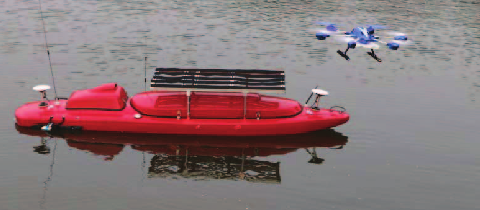
\includegraphics[width=0.62\textwidth]{figures/USVforRescue.pdf}
  \caption{An air-surface system for search in flooded areas under search and rescue missions.\cite{JZhang}}
  \label{fig:USVforRescue}
\end{figure}
\vspace{-6mm}
%
Here the ASV provides long battery life and by carrying the drone, until needed for improved overview, extends reach and duration of each mission.\cite{JZhang}


%%%%%%%%%%Survey%%%%%%%%%%

Another application is for automated survey of an area.
Bathymetric measurements can be used for efficient and safe guidance of marine vessels in shallow waters. 
It is also interesting when studying biological oceanography where it i.e. can help in deciding which areas to protect for preservation of sea life \cite{NOService}. 

%For some types of survey it is required for the ASV to maintain its GPS position while preforming measurements. 
%This requires the system to be able to estimate and counteract external forces, applied to the vessel, keeping it still. 

%A basic functionality of a ASV is to follow a route. 
%This enables to ASV to arrive at a survey side and to preform measurements along a path. 
%%%% https://pdfs.semanticscholar.org/ce94/01a72e78b314f5d2fbbce66f56b217acef1c.pdf
In volcanic countries observations are carried out by volcanologists to provide forecasts and warnings. One observation target is crater lakes. Flash floods and hydrovolcanic explosions can be caused by such lakes. Observing these can help providing information when precautions must be taken and potential evacuation planned.\cite{AWatanabe}
%
\begin{figure}[H]
  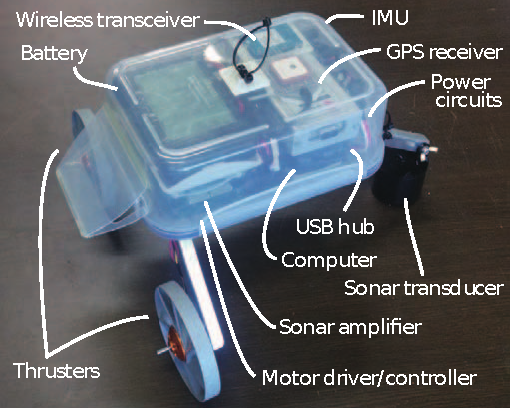
\includegraphics[width=0.35\textwidth]{figures/volcanicLakeUSVwLabels.pdf}
  \caption{Small ASV for taking bathymetric measurements in the Mt. Zao Okama Crater Lake in Japan.\cite{AWatanabe}}
  \label{fig:volcanicLakeUSVwLabels}
\end{figure}
\vspace{-6mm}
%
The small ASV seen in \autoref{fig:volcanicLakeUSVwLabels} is designed to take bathymetric measurements of such lakes and eliminate the need to endanger humans in the process.\cite{AWatanabe}

The USV is made specifically for the Mt. Zao Okama Crater Lake in Japan, where it replaces the need for a manned canoe to enter the volcanic lake situated in high
altitude, strong wind, and restricted area. The bathymetric measurements are used to indicate the amount of water, crater wall caving, and volcanic upthrusts in the lake.\cite{AWatanabe}

An example of a system designed to preform such a task is described in \cite{asv_solar}.
%This implementation achieves such functionality is through a two layer design. 
%An inner controller manipulates the dynamics of the system, while an outer controller is responsible for steering the route through the inner controller. 
This system is able to detect and avoid obstacles in the water, while preforming precision measurements of water quality and greenhouse gases. 
The vessel uses solar cells, which gives the added challenge of controlling the vessel at low speeds, to prevent battery usage during operation for longevity. 
This allows the vessel to autonomously survey relatively large areas without needing to recharge. 

%
%one strength of an ASV is that it can map out an entire stream, whereas manual measurements typicaly will be cumbersome and low in mapping resolution due to accessibility of the stream and time constraints/cost.\\
%for marine survey it can be useful as it can enter narrower and more shallow waters than larger manned vessels would be able to.\\
%the military has also been using ASV's for surveillance.
In this project, the design and implementation of an ASV able to preform bathymetric measurement will be described. 
This will be done using the aauship platform supplied for this project by Aalborg university. 
%In this project the focus is first and foremost the control design, which will be realized with focus on bathymetric measurements. This will constitute a basis for setting up requirements for precision which will determine important parameters in the control design.

    
    %---------- Chapter 2 ---------------------------------------- Problem Analysis
    \chapter{Problem Analysis}
This chapter analyses the scope of the project as well as the requirements that need to be fulfilled.

\section{Scope of the Project}
The goal of this project is to develop a control strategy that can make the autonomous surface vessel be suitable for survey tasks in the water. More specifically, it should be able to perform bathymetric measurements.

The controller design must be able to track references provided by the trajectory planer as well as rejecting disturbances such as possible wind or the effect of the waves. This requires to include a model of the disturbances in the controller design as well as a robust controller capable of handling model uncertainties.

The trajectory planer needs to be able to design a route in the form of waypoints, to send to the controller, to reach all the position needed to perform the different measurements required for the survey. 

One important aspect to be taken into account is the precision of the route tracking, that should be below 10 cm. This requires a positioning system able of providing position data with more precision that the GPS module mounted on the vessel. A test that shows the distribution of the sample from this GPS can be seen in \fxnote{Refer to test with GPS to show it is not enough} For that reason, an RTK GPS is more suitable to enhance the precision of position data.


\section{Requirements} \label{sec:requirements}
To be able to design a working product some functional requirements need to be set and verified at the end of the project once all the design has been carried out.

- tracking of reference position with a precision below 10 cm

- 

    
    %---------- Chapter 3 ---------------------------------------- System Description
    \chapter{System Description}

\begin{figure}[H]
    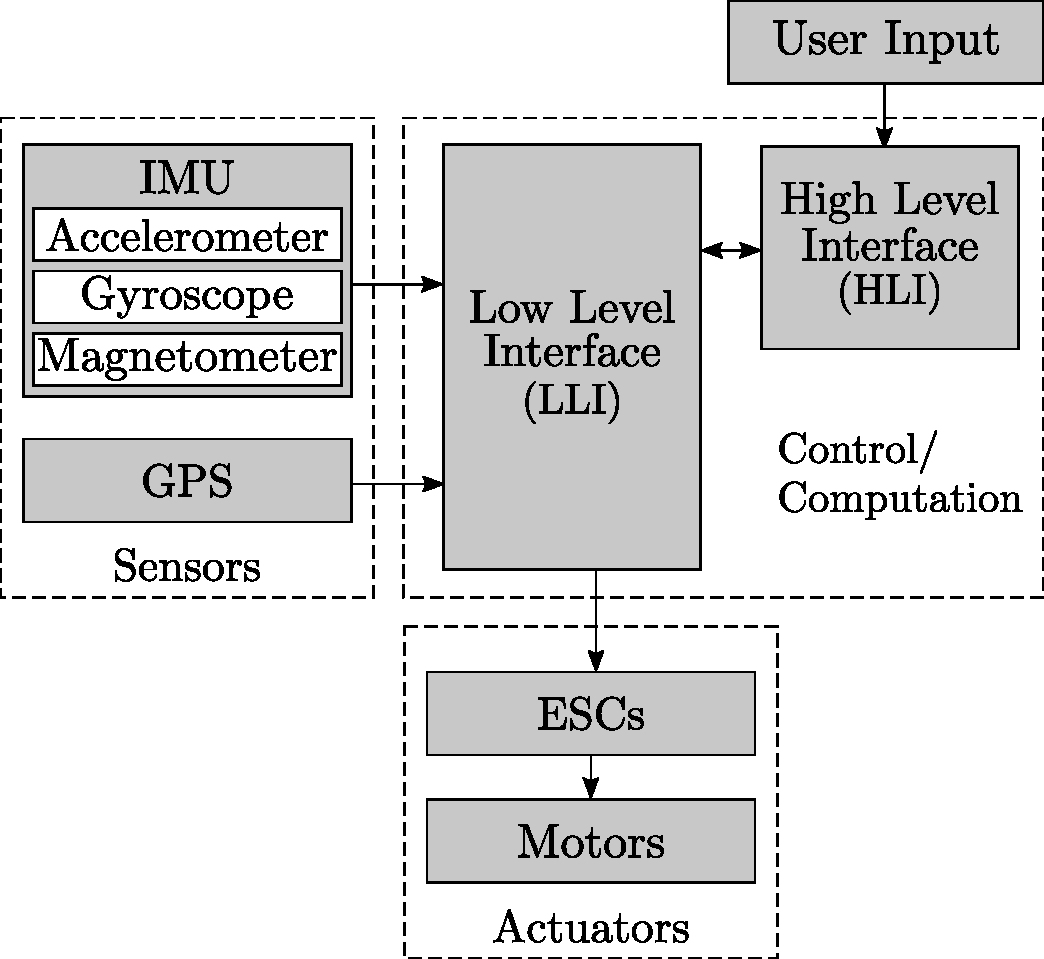
\includegraphics[width=0.6\textwidth]{figures/systemDiagram}
    \caption{}
    \label{fig:systemDiagram}
\end{figure}

Header of the chapter.


    \section{Processing Units}\label{sec:ControlComputation}
The processing units take the sensor data and computes the required actuation output according to the desired motion for the vessel. It is structured in two entities that run in different devices. These entities are the Low Level Interface (LLI) and the High Level Interface (HLI).

\subsection{Low Level Interface} 
The LLI implemented on the vessel runs on a Arduino Mega Development board with and Atmel microcontroller ATMEGA 2560. It is in charge of extracting the sensor data from the IMU and send it to the HLI that runs on the computer. This includes managing the serial communication from the sensors to the Arduino Board and from the Arduino Board to the HLI. 

The LLI also handles the actuators as it receives the command for the thrusters from the HLI and calculates the appropriate PWM so the ESCs make the motors turn at the desired speed.

\subsection{High Level Interface}

The HLI takes care of the control, sensor fusion and trajectory planning algorithms. This includes communicating with the LLI to get sensor data and send commands to the thrusters. 

The HLI is implemented in a ASUS Eee Computer \cite{asus} that runs with Ubuntu 14.04 \cite{ubuntu}. In order to implement the aforementioned algorithms, the Robotic Operating System (ROS) is used. ROS allows programming the different tasks without considering the transmission of data between threads, as this is managed by ROS using its structure of nodes an topics. Besides communication between tasks, it also includes multiple tools and capabilities useful for trajectory planning, computer vision\fxnote{we should probably not mention the vision here?} and others \cite{ROS}.
    \section{Actuation System}
The actuation system present on the vessel is constituted by the thrusters and the ESCs.

\subsection{Thrusters}
The thrusters are the main actuators present on the vessel and they provide a forward force depending on the rotational speed of the motors.

The relationship between the command and the force that they exert have been obtained through an experimental test described in \autoref{app:forceTest}. It is as follows
%
\begin{flalign}
    \mathrm{PWM} = \num{6.6044} \ F + \num{70.0168} \ \ .
    \label{eq:backwardSpeedForce}
\end{flalign}
%
If a negative force is required, they can also rotate in the opposite direction, producing a backwards force that is calculated as 
%
\begin{flalign}
    \mathrm{PWM} = \num{8.5706} \ F - \num{91.9358} \ \ .
    \label{eq:forwardSpeedForce}
\end{flalign}
%

The thrusters are actuated with brushless motors INLINE 750 \num{14.8} V from Graupner. They have two poles with a velocity constant of 1035 rpm$\cdot$kV$^{-1}$ and can operate within \num{7.4} and \num{22.2} V, being the nominal voltage \num{14.8} V. \cite{motors}

\begin{figure}[H]
    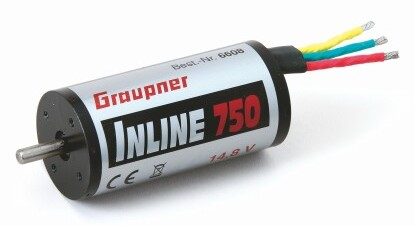
\includegraphics[width=0.4\textwidth]{figures/motor}
    \caption{INLINE 750 \num{14.8} V motor used to produce the thrust in the surface vessel \cite{motors}.}
    \label{fig:motors}
\end{figure}

\subsection{Electronic Speed Controllers}
In order to have the motors turning to the desired rotational speed, electronic speed controllers (ESCs) +70 G\num{3,5} from Graupner are used. The supply voltage ranges from 6 to 25 V and they can handle up to 70 A in continuous current. The reference PWM that comes from the microcontroller translates into a 32kHz PWM signal to the motors. \cite{ESC}

\begin{figure}[H]
    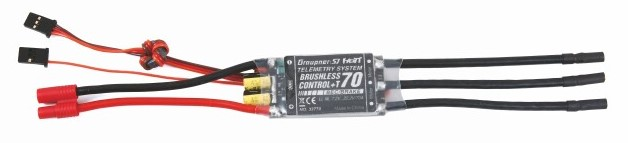
\includegraphics[width=0.8\textwidth]{figures/ESC}
    \caption{Speed controllers +70 G\num{3,5} used to control the  thrusters in the surface vessel \cite{ESC}.}
    \label{fig:ESC}
\end{figure}

%\subsection{Side Thrusters}
%The side thrusters move the vessel sideways but their influence in its motion is limited to low speed maneuvers and they are intended for fine positioning of the vessel. For this reason, they are not utilized in the controller design of the vessel.

    \section{Sensors}\label{sec:sensors}

The control system designed in the vessel requires the presence of sensor data that provide information about the vessel's motion. These are an Inertial Measurement Unit (IMU) and a Global Positioning System (GPS) module.

\subsection{IMU}

The Inertial Measurement Unit installed in the vessel is formed by a triaxial gyroscope with digital range scaling between ±75°/sec, ±150°/sec or ±300°/sec, a triaxial accelerometer with a range of ±18 g and a triaxial magnetometer with a range of ±\num{2.5} gauss. It also contains SPI-compatible serial interface to be able to obtain the data. \cite{IMUDatasheet}
%
\begin{figure}[H]
	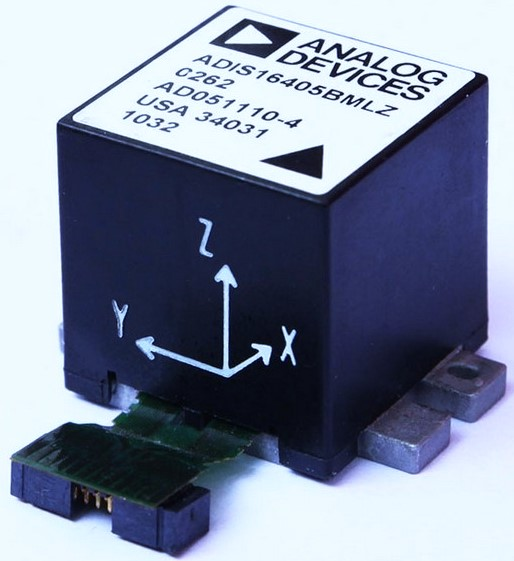
\includegraphics[width=0.3\textwidth]{figures/IMU}
	\caption{ADIS16405BMLZ IMU module mounted in the vessel \cite{IMUFigure}}
	\label{fig:IMU}
\end{figure}
%
The data provided by the IMU is used to estimate both the position and the attitude of the vessel and is extracted in the Low Level Interface through SPI serial communication.

%Triaxial, digital gyroscope with digital range scaling
%±75°/sec, ±150°/sec, ±300°/sec settings
%Tight orthogonal alignment, 0.05°
%Triaxial, digital accelerometer, ±18 g
%Triaxial, digital magnetometer, ±2.5 gauss
%SPI-compatible serial interface
%Embedded temperature sensor
%Single-supply operation: 4.75 V to 5.25 V

\subsection{GPS}
The vessel has a UP-501 GPS Receiver installed. It operates with a update frequency up to 10 Hz and its trasmits the received position data through a serial communication to the Low Level Interface. \cite{GPS}
%
\begin{figure}[H]
	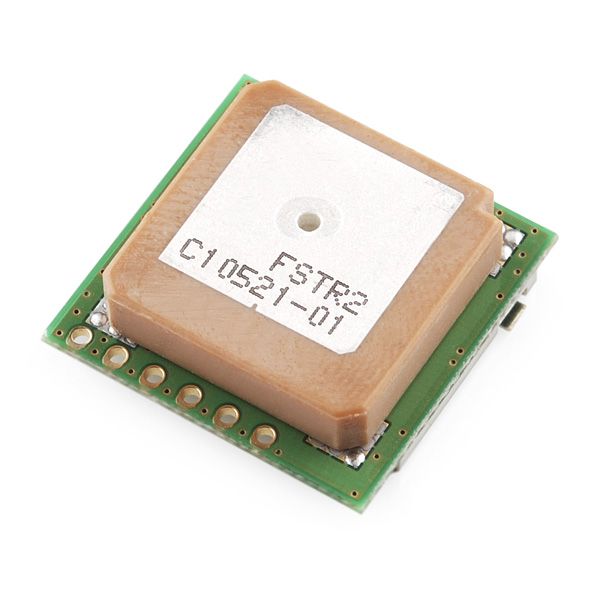
\includegraphics[width=0.3\textwidth]{figures/GPS}
	\caption{UP-501 GPS receiver mounted in the vessel \cite{GPS}.}
	\label{fig:GPS}
\end{figure}
%
As the UP-501 is a standard GPS receiver, its precision is in the range of meters \fxnote{How to prove this?? Maybe make a test.}. This makes it cumbersome to control the position of the vessel using only GPS data, and thus, the GPS and the IMU data is combined to obtained the position of the vessel.

\section{Real Time Kinematic (RTK) GPS}
\fxnote{sources incoming (:}
In addition to the UP-501 module, an Emlid Reach RTK GPS is installed. 
An RTK GPS system consists of two parts, a base station, and a rover.
The base station is set up at a stationary location with a known, precise GPS position.
The rover GPS, mounted on the ASV, measures its location, based on GPS satellites and measurements from the base station.

The base station gets its current position same as the rover using approximately the same satellites. Since the true position of the base is known, so is the error of each measurement. This is then sent as correction data to the rover, where the error is compensated for.

An RTK GPS is able to archive a higher precision than an ordinary GPS by receiving correction data from a base station.
%The correction data is used by the rover to estimate signal disturbances, caused be the signals entering the atmosphere. 
This enables it to increase the precision of the GPS measurements, from 2-5m down to a theoretical precision of a few centimeters.
This data is formatted as an RTCM3 message, which is a protocol designed for this purpose.
\begin{figure}[H]
	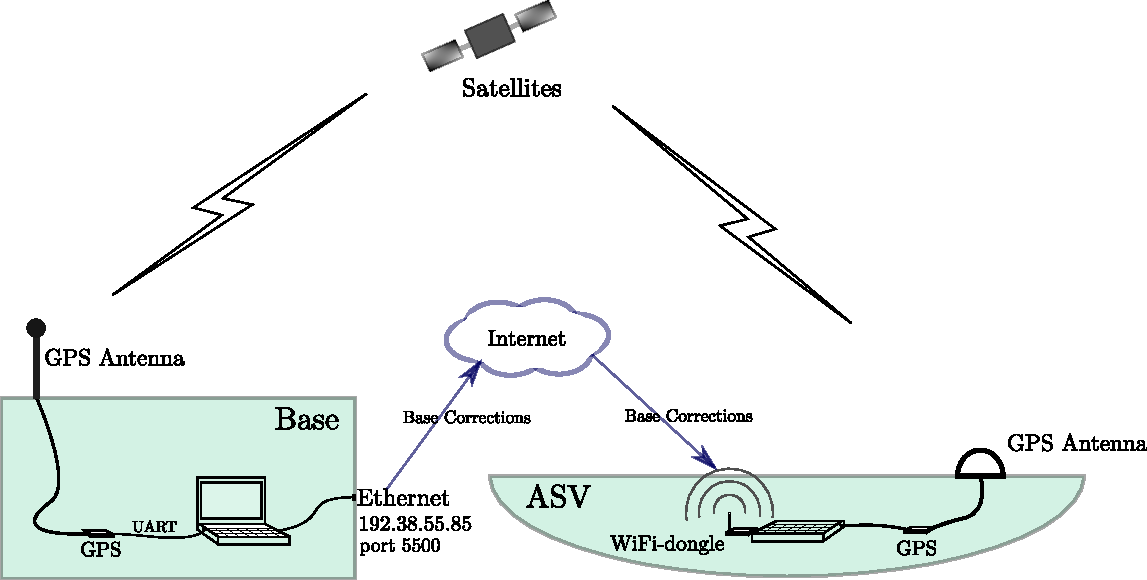
\includegraphics[width=0.6\textwidth]{figures/comunicationSetup.pdf}
	\caption{Overall set up of GPS}
	\label{fig:rtk_GPS}
\end{figure}
\autoref{fig:rtk_GPS} shows how the RTK GPS system is set up. 
The computer runs a Python script which forwards the message to a TCP socket, making it accessible through the Internet. 
The HLI on the vessel connects to this socket and feeds the data to the Rover located on the boat.
For a more detailed description of the setup see \autoref{app:rtk_gps}

    \section{System Additions}
Some changes, including a real time kinematic (RTK) global positioning system (GPS) and communication setup, has been added to the system. A full diagram can be seen in \autoref{fig:systemDiagram2}.
%
\begin{figure}[H]
  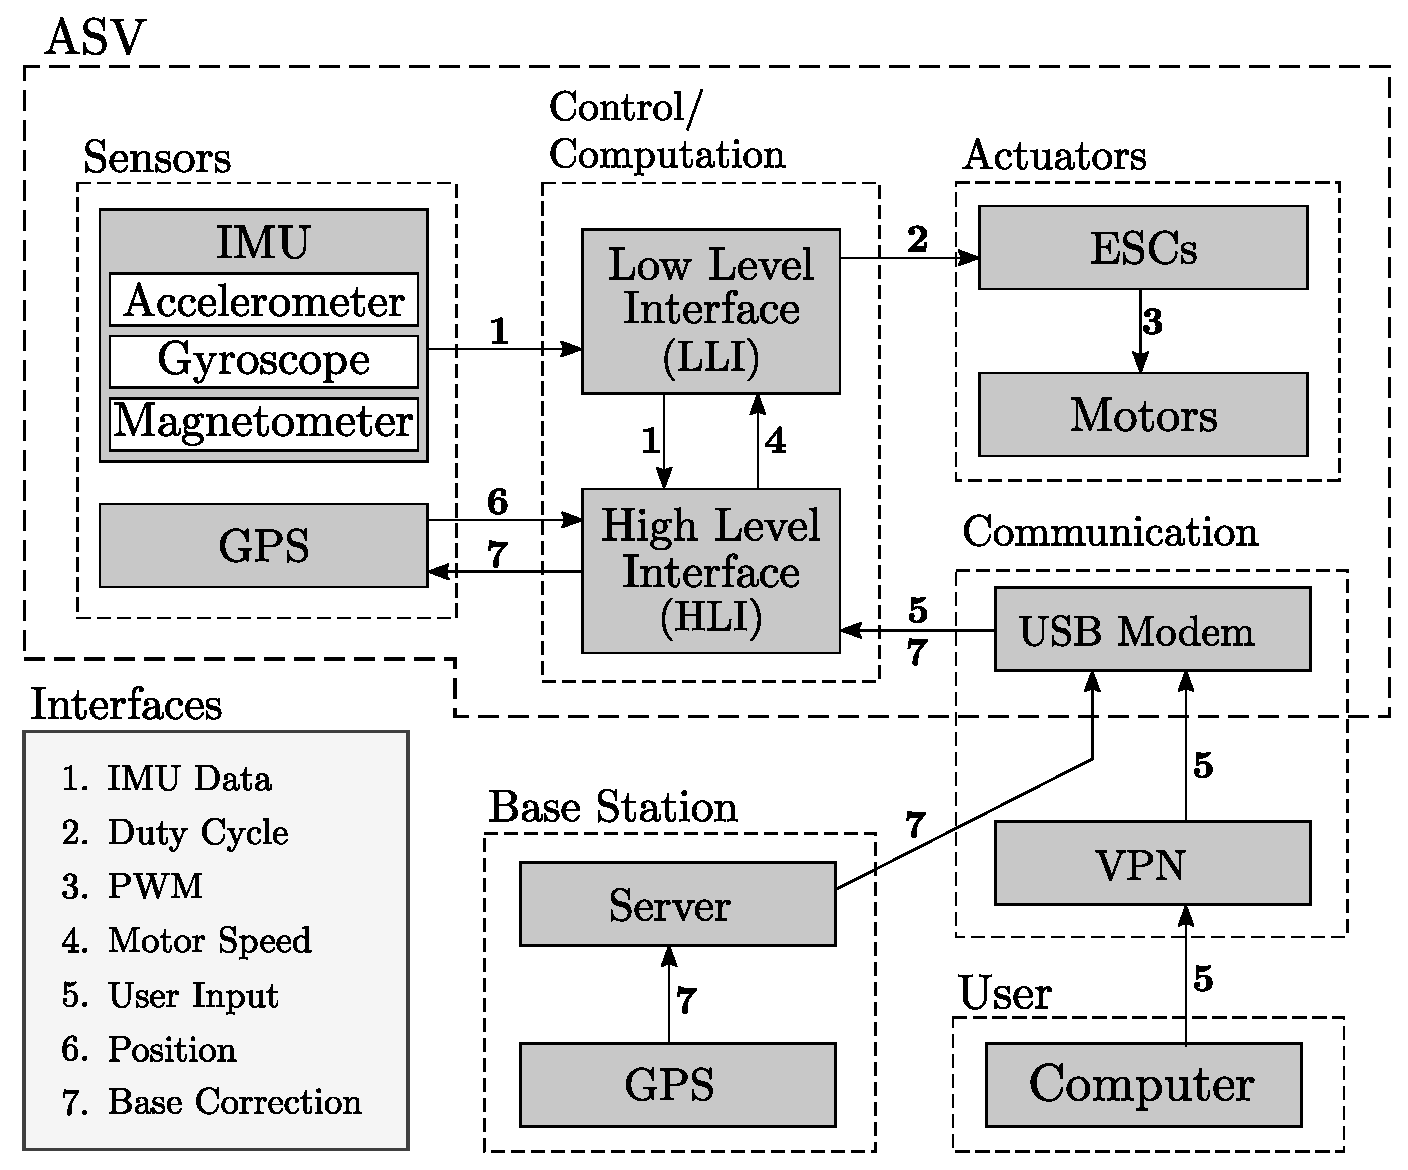
\includegraphics[width=.65\textwidth]{figures/systemDiagram5}
  \caption{A functional diagram of the full system with additions.}
  \label{fig:systemDiagram2}
\end{figure}
%
The RTK GPS system, described in further detail below, is added to obtain better positioning of the ASV. This feature is necessary to accurately map the seabed of the Port of Aalborg with the standards mentioned in \autoref{sec:designconsiderations}.
%This is necessary to obtain sub-meter positioning, without which the control design would have little impact on the performance of the system.\\

Additionally a virtual private network (VPN) server and a USB modem is used to provide user input when the ASV and user are not on the same closed network. This makes it possible to access the ASV through the cellular network and thus eliminates potential problems with regards to range between user and ASV.

\subsection{RTK GPS}
An RTK GPS system consists of two parts, a base station, and a  mobile unit called rover.

The base station is set up at a stationary location with a known, precise GPS position. The rover GPS, mounted on the ASV, measures its location, based on GPS satellites and measurements from the base station. \cite{EmlidRTK}

The modules used in this project, both for the base and the rover, are Emlid Reach RTK GPS, see \autoref{fig:emlidReach}.

\begin{figure}[H]
  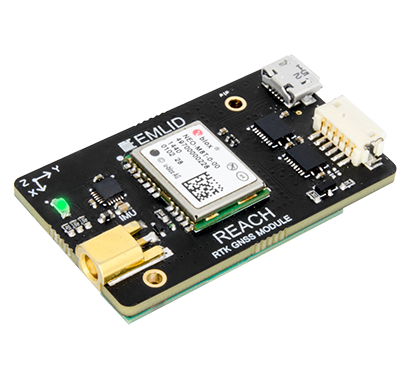
\includegraphics[width=0.27\textwidth]{figures/emlidReach}
  \caption{Emlid Reach RTK GPS module.\cite{EmlidReachDocs}}
  \label{fig:emlidReach}
\end{figure}

The base station gets its current position same as the rover using the same satellites. Since the true position of the base is known, so is the error of each measurement. This is then sent as correction data to the rover, where the error is compensated for. \fxnote{Correct description}

An RTK GPS is able to achieve a higher precision than an ordinary GPS by receiving correction data from a base station, improving from 2-5 m down to a theoretical precision of a few centimeters. \cite{EmlidRTK}

%This data is formatted as an RTCM3 message, which is a protocol designed for this purpose.

\autoref{fig:rtk_GPS} shows how the RTK GPS system is set up. 

\begin{figure}[H]
	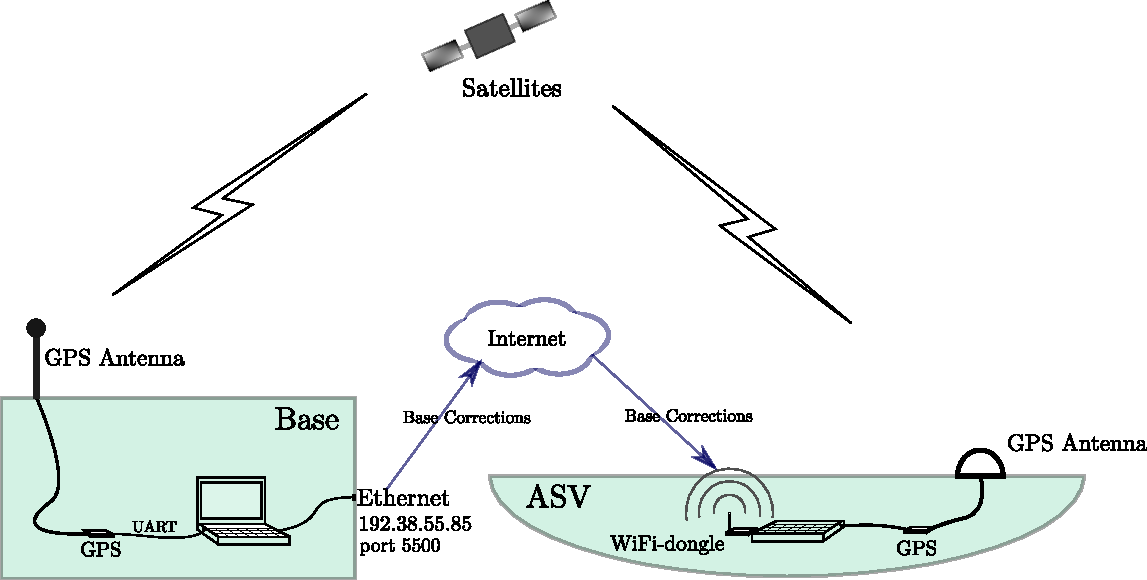
\includegraphics[width=0.8\textwidth]{figures/comunicationSetup.pdf}
	\caption{Overall set up of the GPS.}
	\label{fig:rtk_GPS}
\end{figure}

The base computer forwards the message to a TCP socket, making it accessible through the Internet. The HLI on the vessel connects to this socket and feeds the data to the rover located on the boat. For a more detailed description of the setup see \autoref{app:rtk_gps}.

    
    %---------- Chapter 4 ---------------------------------------- Modeling
    \chapter{System Model} \label{chap:model}
The model of the surface vessel is based in the methods presented in \cite{TFossen}, where the main dynamic effects regarding the behavior of the vessel are taken into account and  described in order to generate a model that serves as a basis for control design and simulations.


    \section{Background}
The model of the surface vessel is based in the hydrodynamic modeling presented in \cite{TFossen}, where the principal effects that need to be taken into account are described.

In this section, the different contributions are summarized and related to the vessel at hand.

\subsection{Reference Frames}
To describe the orientation and position of the surface vessel two coordinate frames are used, the body frame and an inertial frame. For operations in a local area, with longitude and latitude approximately constants (flat navigation) a NED system (North-East-Down) can be assumed as an inertial frame where Newton's physics will apply \cite[p. 17]{TFossen}.

To distinguish between the two frames, the body frame is denoted by a subindex "$_\mathrm{b}$", and the inertial frame with subindex "$_\mathrm{n}$". In \autoref{fig:refFrame}, a diagram of the surface vessel with the notation used can be seen.

\begin{figure}[H]
    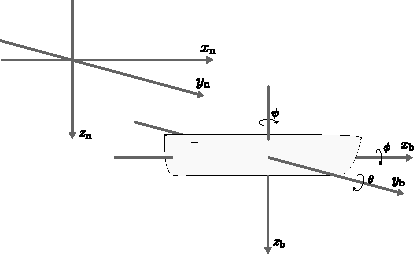
\includegraphics[width=0.6\textwidth]{figures/boat3D}
    \caption{$x_\mathrm{b}$, $y_\mathrm{b}$ and $z_\mathrm{b}$ refer to the position with respect to the body coordinate frame, while $x_\mathrm{n}$, $y_\mathrm{n}$ and $z_\mathrm{n}$ describe it with respect to the inertial frame. $\phi$, $\theta$ and $\psi$ refer to the rotation around $x_\mathrm{b}$, $y_\mathrm{b}$ and $z_\mathrm{b}$, respectively.}
    \label{fig:refFrame}
\end{figure}


The transformation from the body frame to the inertial can be done through a rotation matrix, \eqref{eq:RotMatrix}, which describes a total rotation in terms of three consecutive rotations.

In this case the rotation matrix is composed with a 1-2-3 convention, that is, first a rotation around $x_{\mathrm{b}}$, then around $y_{\mathrm{b}}$ and finally around $z_{\mathrm{b}}$ \cite[p. 22]{TFossen}.

\begin{minipage}{0.32\linewidth}
    \begin{flalign}
    \vec{R}_\mathrm{X} &=
    \begin{bmatrix}
    1 & 0      & 0       \\ 
    0 & c\phi  & -s\phi  \\ 
    0 & s\phi  & c\phi   \nonumber  
    \end{bmatrix} 	\label{eq:RotMatrix1}
    \end{flalign}
\end{minipage}\hfill
\begin{minipage}{0.32\linewidth}
    \begin{flalign}
    \vec{R}_\mathrm{Y} &=
    \begin{bmatrix}
    c\theta  & 0  & s\theta  \\ 
    0          & 1  & 0      \\ 
    -s\theta & 0  & c\theta  \nonumber 
    \end{bmatrix} 	\label{eq:RotMatrix2}
    \end{flalign}
\end{minipage}\hfill
\begin{minipage}{0.32\linewidth}
    \begin{flalign}
    \vec{R}_\mathrm{Z} &=
    \begin{bmatrix}
    c\psi & -s\psi  & 0  \\ 
    s\psi & c\psi   & 0  \\ 
    0       & 0         & 1  \nonumber 
    \end{bmatrix} 	\label{eq:RotMatrix3}
    \end{flalign}
\end{minipage}\hfill
\small
\begin{flalign}
\vec{R}^\mathrm{n}_\mathrm{b} = \vec{R}_Z \vec{R}_Y \vec{R}_X =
\begin{bmatrix}
c\theta c\psi  & s\phi s\theta c\psi -c\phi s\psi  & c\phi s\theta c\psi + s\phi s\psi  \\ 
c\theta s\psi  & s\phi s\theta s\psi + c\phi c\psi & c\phi s\theta s\psi - s\phi c\psi  \\ 
-s\theta         & s\phi c\theta                           & c\phi c\theta
\end{bmatrix} 	\label{eq:RotMatrix}
\end{flalign}
\normalsize
%
\begin{where}
    \va{\vec{R}_\mathrm{X}}{is the matrix describing a rotation around the $x_\mathrm{b}$ axis}{}
    \va{\vec{R}_\mathrm{Y}}{is the matrix describing a rotation around the $y_\mathrm{b}$ axis}{}
    \va{\vec{R}_\mathrm{Z}}{is the matrix describing a rotation around the $z_\mathrm{b}$ axis}{}
    \va{\vec{R}^\mathrm{n}_\mathrm{b}}{is the total rotation matrix}{}
\end{where}

Note that due to the size of the matrix sine and cosine are denoted $s$ and $c$ respectively.

To describe a vector in the inertial frame given its description in the body frame, a matrix-vector multiplication can be done as follows:
%
\begin{flalign}
v_{\mathrm{n}}=\vec{R}^\mathrm{n}_\mathrm{b}v_\mathrm{b} 
\end{flalign}
\begin{where}
    \va{v_{\mathrm{n}}}{is a column vector that contains the description with respect to the inertial frame}{}
    \va{v_{\mathrm{b}}}{is a column vector that contains the description with respect to the body frame}{}
\end{where}

If the inverse computation is needed, it can be done following the same procedure using $\vec{R}^\mathrm{n\ T}_\mathrm{b}$ as the rotation matrix.    

\subsection{Rigid Body Dynamics}

The first step to model the motion of the surface vessel is to look at its rigid body dynamics. They are described assuming that the center of gravity of the boat coincides with the origin of the body coordinate frame.

The translational movement can be analyzed using Newton's second law, where the acceleration of the vessel is related to the applied forces.
%
\begin{flalign}
\sum F=m \ddot{x}
\end{flalign}
%
In the case of the rotational movement, the motion is describe using the Newton's second law applied to rotational movement, where the torques applied to the system influence the angular acceleration in each axis.
%
\begin{flalign}
\sum \tau=I \ddot{\theta}
\end{flalign}
%
%The movement can be influence by the Coriolis effect, due to the fact that the body coordinate frame rotates with respect to the inertial frame. This effect, however, can be neglected in the case of a small vehicle that moves slow such as the vessel at hand \finite{find source}.
This movement is subject to the Coriolis effect, which appear if the vessel is not rotating around the axis with least- or highest- inertial axis.
The influence of this force is small if the vessel rotates at low speeds, hence it have been neglected in the model.

\subsection{Hydrostatics}

The hydrostatics describe what forces and torques are applied on the surface vessel by the volume of fluid displaced when floating on water. The force induced upon the vessel is called buoyancy force and it is applied to the center of buoyancy.  

The buoyancy force acts in the negative $z_\mathrm{n}$ direction as seen in
%
\begin{flalign}
B = \rho g (V + \Delta V(z))
\end{flalign}
\begin{where}
    \va{\rho}{is the density of the fluid in which the vessel floats}{kg m^{-3}}
    \va{g}{is the gravitational acceleration}{m s^{-2}}
    \va{V}{is the volume of fluid displaced by the surface vessel}{m^3}
    \va{\Delta V}{is the change in volume of fluid displaced by the surface vessel}{m^3}
    \va{B}{is the buoyancy force}{N}
\end{where}

When the vessel floats, the gravity force cancels out $ \rho g V $ of the buoyancy force, making the contribution of the latest along $x_\mathrm{b}$, $y_\mathrm{b}$ and $z_\mathrm{b}$ directions dependent only on the variation with respect to the equilibrium flotation point.
This result is seen in 
%
\begin{flalign}
F_{z_\mathrm{n}} = mg - \rho g V -\rho g  \Delta V(z) = -\rho g  \Delta V(z) 
\end{flalign}
\begin{where}
    \va{F_{z_\mathrm{n}}}{is the summation of forces along the $z_\mathrm{n}$ direction}{N}
\end{where}

The change in volume can be expressed as in \autoref{eq:deltaV}. The water plane of the vessel is not considered to vary significantly with change in vertical position, thus the approximation seen in the equation is applied.
%
\begin{flalign}
\Delta V(z) = \int_{0}^{z_\mathrm{N}}A_\mathrm{wp}(\zeta)d\zeta \approx A_\mathrm{wp}z_\mathrm{n}
\label{eq:deltaV}
\end{flalign}
\begin{where}
    \va{A_\mathrm{wp}}{is the water plane area of the vessel}{m^2}
\end{where}

The contribution along the body frame directions is calculated as a function of the $\phi$ and $\theta$ angles in  
%
\begin{flalign}
F_{x_\mathrm{b}} &= -\rho g A_\mathrm{wp}z_\mathrm{n} (-\sin \theta)  \\
F_{y_\mathrm{b}} &= -\rho g A_\mathrm{wp}z_\mathrm{n} (\cos \theta \sin \phi)  \\
F_{z_\mathrm{b}} &= -\rho g A_\mathrm{wp}z_\mathrm{n} (\cos \theta \cos \phi) 
\label{eq:forcez}
\end{flalign}

If the variations of $\phi$ and $\theta$ are small, the contribution of the buoyancy force in the $x_\mathrm{b}$ and $y_\mathrm{b}$ directions can be neglected and not included in the final model of the vessel. \cite[pp. 62-67]{TFossen}

The buoyancy force also contributes with some torques around the different axis in the body coordinate frame. This occurs as the center of buoyancy in general is not aligned with the center of gravity, generating some restoring torques on the vessel. These torques are dependent on the gravity and the buoyancy force. As the contribution of the term $\rho g \Delta V$ is small compared to that of $\rho g V$, only the latter is considered in the model.  \cite[pp. 62-67]{TFossen}
%
\begin{flalign}
T_{\phi} &= -\rho g V \overline{GM}_{\mathrm{T}} \sin \phi (\cos \theta \cos \phi)   
\label{eq:torqphi} \\
T_{\theta} &= -\rho g V \overline{GM}_{\mathrm{L}} \sin \theta (\cos \theta \cos \phi) 
\label{eq:torqtheta}
\end{flalign}
\begin{where}
    \va{T_{\phi}}{is the restoring torque due to the buoyancy force in the $\phi$ direction}{Nm}
    \va{T_{\theta}}{is the restoring torque due to the buoyancy force in the $\theta$ direction}{Nm}
    \va{\overline{GM}_\mathrm{T}}{is the transverse metacentric height}{m}
    \va{\overline{GM}_\mathrm{L}}{is the longitudinal metacentric height}{m}
\end{where}

The metacentric heights are the distances between the center of gravity and the metacenter of the vessel. The metacenter position is related with the position of the center of gravity and that of the center of buoyancy. \cite[pp. 65-67]{TFossen}
%equations in the book page 78

\subsection{Hydrodynamics}
The hydrodynamic forces induced in the surface vessel are mainly caused by two terms. The added mass and the viscous damping.

The added mass induces forces that originate from the vessel imposing some energy in the surrounding fluid when it moves through it. The force generated is dependent on the acceleration of the vessel. \fxnote{what to do here??}

The viscous damping is a combination of several factors, namely, skin friction, wave drift damping and vortex shedding \cite[p. 122]{TFossen}. This type of damping appears in the equations as coefficients that multiply, with negative sign, the different translational and angular velocities that define the movement of the vessel. For each degree of freedom it is expressed as
%
\begin{flalign}
D_{\dot{x}_\mathrm{b}} &= - d_{\dot{x}_\mathrm{b}}  \dot{x}_\mathrm{b} \\
D_{\dot{y}_\mathrm{b}} &= - d_{\dot{y}_\mathrm{b}}  \dot{y}_\mathrm{b} \\
D_{\dot{z}_\mathrm{b}} &= - d_{\dot{z}_\mathrm{b}}  \dot{z}_\mathrm{b} \\
D_{\dot{\phi}} &= - d_{\dot{\phi}}                  \dot{\phi} \\
D_{\dot{\theta}} &= - d_{\dot{\theta}}              \dot{\theta} \\
D_{\dot{\psi}} &= - d_{\dot{\psi}}                  \dot{\psi}  \\
\end{flalign}
\begin{where}
    \va{D_{i}}{is the damping force or torque due to viscous damping.}{}
    \va{d_{i}}{is the viscous damping coefficient.}{}
\end{where}

This equation consider that the viscous friction is linear, this assumption can be done for vessel speeds lower than 2 m/s \cite[p. 138]{TFossen}. 

    \section{Model Equations}   
The final model equations are presented in this section, and are described relative to the body frame, meaning that all movement is relative to the vessel.
\autoref{fig:boat3DForces} and \ref{fig:boat2D} show a diagram of the vessel.
\begin{figure}[H]
    \captionbox
    {
        Diagram of the vessel, where the forces applied by the motors are shown.
        \label{fig:boat3DForces}
    }
    {
        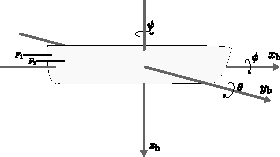
\includegraphics[width=.54\textwidth]{figures/boat3DForces}
    }
    \hspace{5pt}
    \captionbox
    {
        Top view of the vessel, where the distances needed for the model equations are also presented.
        \label{fig:boat2D}
    }
    {
        \hspace{1.1cm} 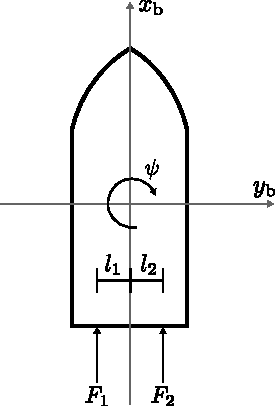
\includegraphics[width=.24\textwidth]{boat2D} \hspace{1.1cm}
    }
\end{figure}

The translational movement of the vessel is described by \autoref{eq:x_pos_model}, \ref{eq:y_pos_model} and \ref{eq:z_pos_model}.
The model includes the forces applied by the motors and the damping, that create an acceleration in the vessel as
%
\begin{flalign}
	m \ddot{x}_\mathrm{b} &=  F_\mathrm{1} + F_\mathrm{2}  - d_{\dot{x}_\mathrm{b}} \dot{x}_\mathrm{b} + F_{x_\mathrm{b}}
    \label{eq:x_pos_model} \ ,\\
    m \ddot{y}_\mathrm{b} &=  -d_{\dot{y}_\mathrm{b}} \dot{y_\mathrm{b}} + F_{y_\mathrm{b}}
    \label{eq:y_pos_model} \ ,\\
    m \ddot{z}_\mathrm{b} &=  -d_{\dot{z}_\mathrm{b}}\dot{z_\mathrm{b}} + F_{z_\mathrm{b}} \ . \label{eq:z_pos_model}
\end{flalign}
%
\begin{where}
	\va{m}{is the mass of the vessel}{kg}
    \va{\ddot{x}_\mathrm{b}}{is the acceleration in the $x_\mathrm{b}$ direction}{m \cdot s^{-2}}
    \va{\ddot{y}_\mathrm{b}}{is the acceleration in the $y_\mathrm{b}$ direction}{m \cdot s^{-2}}
    \va{\ddot{z}_\mathrm{b}}{is the acceleration in the $z_\mathrm{b}$ direction}{m \cdot s^{-2}}
    \va{\dot{x}_\mathrm{b}}{is the velocity in the $x_\mathrm{b}$ direction}{m \cdot s^{-1}}
    \va{\dot{y}_\mathrm{b}}{is the velocity in the $y_\mathrm{b}$ direction}{m \cdot s^{-1}}
    \va{\dot{z}_\mathrm{b}}{is the velocity in the $z_\mathrm{b}$ direction}{m \cdot s^{-1}}
    \va{F_{1,2}}{are the forces applied by each motor}{N}
\end{where}

%The virtual mass components are the added mass from the displaced water in the respective direction plus the mass of the vessel. This value is different for each axis, as the difference in shape drags a different amount of water.
    
The rotational movement of the vessel is described by \autoref{eq:phi_model}, \ref{eq:theta_model} and \ref{eq:psi_model}.
%
\begin{flalign}
    I_\mathrm{x}\ddot{\phi} &= -d_{\dot{\phi}} \dot{\phi} + T_\mathrm{\phi}  \ ,
    \label{eq:phi_model} \\
    I_\mathrm{y}\ddot{\theta} &= -d_{\dot{\theta}} \dot{\theta} + T_\mathrm{\theta}  \ ,
    \label{eq:theta_model} \\
    I_\mathrm{z}\ddot{\psi} &= F_\mathrm{1}l_\mathrm{1} - F_\mathrm{2} l_\mathrm{2} - d_{\dot{\psi}} \dot{\psi} \ . \label{eq:psi_model}
\end{flalign}
%
\begin{where}
    \va{I_\mathrm{x}}{is the inertia around the $x_\mathrm{b}$ axis}{kg \cdot m^2}
    \va{I_\mathrm{y}}{is the inertia around the $y_\mathrm{b}$ axis}{kg \cdot  m^2}
    \va{I_\mathrm{z}}{is the inertia around the $z_\mathrm{b}$ axis}{kg \cdot  m^2}
    \va{\ddot{\phi}}{is the angular acceleration around the $x_\mathrm{b}$ axis}{rad\cdot s^{-2}}
    \va{\ddot{\theta}}{is the angular acceleration around the $y_\mathrm{b}$ axis}{rad \cdot s^{-2}}
    \va{\ddot{\psi}}{is the angular acceleration around the $z_\mathrm{b}$ axis}{rad \cdot s^{-2}}
    \va{\dot{\phi}}{is the angular velocity around the $x_\mathrm{b}$ axis}{rad \cdot s^{-1}}
    \va{\dot{\theta}}{is the angular velocity around the $y_\mathrm{b}$ axis}{rad \cdot s^{-1}}
    \va{\dot{\psi}}{is the angular velocity around the $z_\mathrm{b}$ axis}{rad \cdot s^{-1}}
    \va{l_1}{is the perpendicular distance from motor 1 to the center of gravity}{m}
    \va{l_2}{is the perpendicular distance from motor 2 to the center of gravity}{m}
\end{where}

Similar to the translational equations, only one axis is controllable. This is, however, not a problem in practice, since the vessel is stable by nature and it can be controlled even being an underactuated vehicle \cite[pp. 235-239]{TFossen}.

    \section{Linearization of Model Equations}\label{sec:linearizationModel}
The model equations need to be linearized to design a controller using linear techniques. This is done using the first order Taylor approximation around an equilibrium point as seen in 
%
\begin{flalign}
    f(x) &\approx f(\overline{x}) + f'(\overline{x}) (x-\overline{x})  \rightarrow\ \tilde{f}(x) \approx f'(\overline{x}) \tilde{x} \ .
    \label{taylor}
\end{flalign}

In this equation, $\overline{x}$ represents the equilibrium point and $\tilde{x}$ the change from the equilibrium point.

The equilibrium point must fulfill that all the derivatives of the states are zero, in this case the velocities and accelerations. This implies that the resulting forces and torques must be zero. 

To apply the approximation, the function must be differentiated with respect to each of the present variables, and once linearized, the function is expressed in terms of variations from the equilibrium point.
%
\begin{flalign}
    f &= f(x_1,x_2,...,x_\mathrm{n}) \nonumber \ ,\\
    \tilde{f}&=\frac{\partial f}{\partial x_1}\bigg|_{\overline{x}_1,\overline{x}_2,...,\overline{x}_n}\ \tilde{x}_1 + \frac{\partial f}{\partial x_2}\bigg|_{\overline{x}_1,\overline{x}_2,...,\overline{x}_n}\ 
    \tilde{x}_2+...+ \frac{\partial f}{\partial x_n}\bigg|_{\overline{x}_1,\overline{x}_2,...,\overline{x_n}}\ \tilde{x}_\mathrm{n} \ . \nonumber
    \label{eq:dummytaylor}
\end{flalign}
%
In the case of the vessel, the only nonlinear terms are the restoring forces and torques. They can be linearized, giving the following results
\begin{flalign}
    \tilde{F}_{x_\mathrm{b}} &= 0  \label{eq:forcexlin} \ ,\\
    \tilde{F}_{y_\mathrm{b}} &= 0  \label{eq:forceylin} \ ,\\
    \tilde{F}_{z_\mathrm{b}} &= -\rho g A_\mathrm{wp} \tilde{z}_\mathrm{n} \label{eq:forcezlin} \ , \\
 	\tilde{T}_{\phi} &= -\rho g V \overline{GM_{T}}\cdot \tilde{\phi} \label{eq:torquephilinar} \ , \\
    \tilde{T}_{\theta} &= -\rho g V \overline{GM_{L}}\cdot \tilde{\theta} \ .\label{eq:torquethetalinar}   
\end{flalign}
%
From now on, the linearized variables are represented without the symbol "$\sim$", to avoid excessive notation, even though they refer to changes with respect to the the equilibrium point.

The model equations including these linearized terms end up being
%
\begin{flalign}
 	m_\mathrm{x} \ddot{x}_\mathrm{b} &=  F_\mathrm{1} + F_\mathrm{2}  - d_{\dot{x}_\mathrm{b}} \dot{x}_\mathrm{b}
     \label{eq:x_pos_model_lin} \ , \\
    m_\mathrm{y} \ddot{y}_\mathrm{b} &=  -d_{\dot{y}_\mathrm{b}} \dot{y_\mathrm{b}}
     \label{eq:y_pos_model_lin} \ , \\
    m_\mathrm{z} \ddot{z}_\mathrm{b} &=  -d_{\dot{z}_\mathrm{b}}\dot{z_\mathrm{b}} -\rho g A_\mathrm{wp} \tilde{z}_\mathrm{n} \label{eq:z_pos_model_lin} \ ,  \\
    I_\mathrm{x}\ddot{\phi} &= -d_{\dot{\phi}} \dot{\phi} - \rho g V \overline{GM_{T}}\cdot \phi
    \label{eq:phi_model_limn} \ , \\
    I_\mathrm{y}\ddot{\theta} &= -d_{\dot{\theta}} \dot{\theta} - \rho g V \overline{GM_{L}}\cdot \theta
    \label{eq:theta_model_lin} \ , \\
    I_\mathrm{z}\ddot{\psi} &= F_\mathrm{1}l_\mathrm{1} - F_\mathrm{2} l_\mathrm{2} - d_{\dot{\psi}} \dot{\psi} \ . \label{eq:psi_model_lin}
\end{flalign}



%\begin{flalign}
%    m_\mathrm{x} \ddot{x}_\mathrm{b} &=  F_\mathrm{1} + F_\mathrm{2}  - d_\mathrm{x} \dot{x}_\mathrm{b} + m_\mathrm{y} \dot{y_\mathrm{b}} \dot{\psi} - m_\mathrm{z} \dot{z}_\mathrm{b} \dot{\theta} - F_\mathrm{x}
%    \label{eq:x_pos_model} \\
%    m_\mathrm{y} \ddot{y_\mathrm{b}} &=  -d_\mathrm{y}\dot{y_\mathrm{b}}-m_\mathrm{x}\dot{x_\mathrm{b}}\dot{\psi}+m_\mathrm{z}\dot{z_\mathrm{b}}\dot{\phi}-F_\mathrm{y}
%    \label{eq:y_pos_model} \\
%    m_\mathrm{z} \ddot{z_\mathrm{b}} &=  -d_\mathrm{z}\dot{z_\mathrm{b}}+ m_\mathrm{b}\dot{x_\mathrm{b}}\dot{\theta}-m_\mathrm{y}\dot{y_\mathrm{b}} \dot{\phi}-F_\mathrm{z} \label{eq:z_pos_model}
%\end{flalign}
%
%\begin{flalign}
%    I_\mathrm{x}\ddot{\phi} &= -d_\mathrm{\phi} \dot{\phi}-(m_\mathrm{z}-m_\mathrm{y}) \dot{z}_\mathrm{b} \dot{y}_\mathrm{b}-(I_\mathrm{z}-I_\mathrm{y}) \dot{\theta } \dot{\psi}+T_\mathrm{\phi}  
%    \label{eq:x_inert_model} \\
%    I_\mathrm{y}\ddot{\theta} &= -d_\mathrm{\theta} \dot{\theta}-(m_\mathrm{z}-m_\mathrm{x}) \dot{x}_\mathrm{b} \dot{y}_\mathrm{b}-(I_\mathrm{x}-I_\mathrm{z}) \dot{\phi} \dot{\psi}+T_\mathrm{\theta}  
%    \label{eq:y_inert_model} \\
%    I_\mathrm{z}\ddot{\psi} &= -d_\mathrm{\psi} \dot{\psi}-(m_\mathrm{y}-m_\mathrm{x}) \dot{x}_\mathrm{b}\dot{y}_\mathrm{b}-(I_\mathrm{z}-I_\mathrm{y})\dot{\psi}\dot{\theta}+F_\mathrm{1}l_\mathrm{1}+F_\mathrm{2}l_\mathrm{2}+T_\mathrm{\psi} \label{eq:z_inert_model}
%\end{flalign}

    \section{Model Verification}\label{sec:modelVerification}
The parameters used in the final model are taken form previous work on the vessel \cite{thesis}.

\begin{table}[H]
    \begin{tabular}{|c|c|c|}    
        \hline %-----------------------------------------------------------------------------------
        \textbf{Parameter} &\textbf{Value} & \textbf{Units} \\
        \hline %-----------------------------------------------------------------------------------
        $m$  & 13 & kg \\
        $d_{\dot{x}_\mathrm{b}}$  & 2.86 & N$\cdot$m$^{-1}$$\cdot$s \\
        $d_{\dot{y}_\mathrm{b}}$  & 32.5 & N$\cdot$m$^{-1}$$\cdot$s \\
        $I_\mathrm{x}$  & 0.0654 & kg$\cdot$m$^2$ \\
        $I_\mathrm{y}$  & 1.0892 & kg$\cdot$m$^2$ \\
        $I_\mathrm{z}$  & 1.1067 & kg$\cdot$m$^2$ \\
        $d_{\dot{\phi}}$ & 0.1094 &  N$\cdot$m$\cdot$rad$^{-1}$$\cdot$s\\
        $d_{\dot{\theta}}$ & 7.2030 & N$\cdot$m$\cdot$rad$^{-1}$$\cdot$s \\
        $d_{\dot{\psi}}$ & 0.2228 & N$\cdot$m$\cdot$rad$^{-1}$$\cdot$s \\
        $l_1$ & 0.05 & m \\
        $l_2$ & 0.05 & m \\
        $\rho g V \overline{GM_{T}}$ & 6.9736 & N$\cdot$m\\
        $\rho g V \overline{GM_{T}}$ & 131.8316 & N$\cdot$m\\
        \hline %-----------------------------------------------------------------------------------
    \end{tabular}
\end{table}

As it can be seen, the parameters corresponding to the $z_\mathrm{b}$ direction are not presented, since \autoref{eq:z_pos_model_lin} is not used neither for the control design nor for the sensor fusion.

To verify the model a test is carried out. Two constant but different forces are applied to see the turning behavior of the real vessel, as seen in \autoref{app:modelVerification}. The data is then compared to the simulated model when applying the same inputs, and the results can be seen in \autoref{fig:turn} and \ref{fig:turn_time}.

\begin{figure}[H]
    \captionbox 
    {   
        Position of the vessel in the $x_\mathrm{n}$-$y_\mathrm{n}$ plane given by the model simulation and the GPS data.
        \label{fig:turn}
    }                                                                 
    {                                                                  
        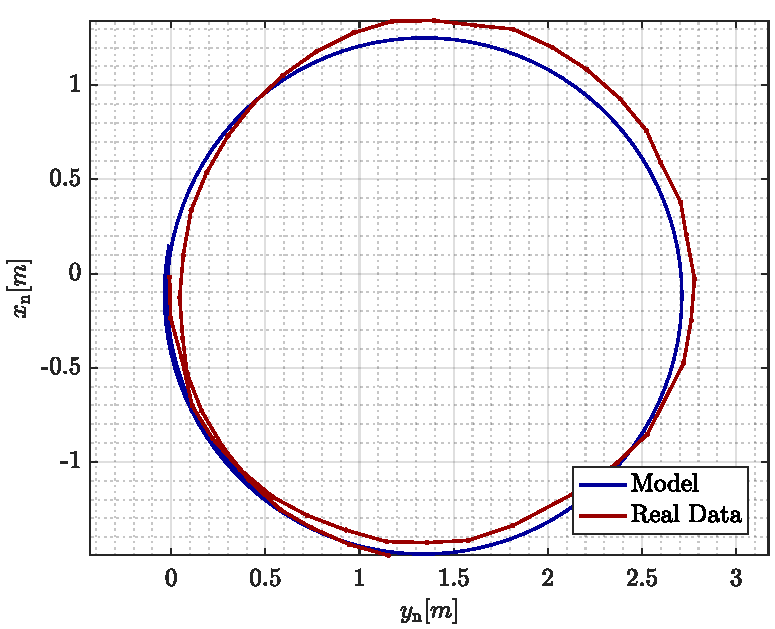
\includegraphics[width=.45\textwidth]{figures/turn}         
    }                                                                    
    \hspace{5pt}                                                          
    \captionbox  
    {      
        $x_\mathrm{n}$ and $y_\mathrm{n}$ with respect to time, both simulated and real.
        \label{fig:turn_time}
    }                                                                        
    {
        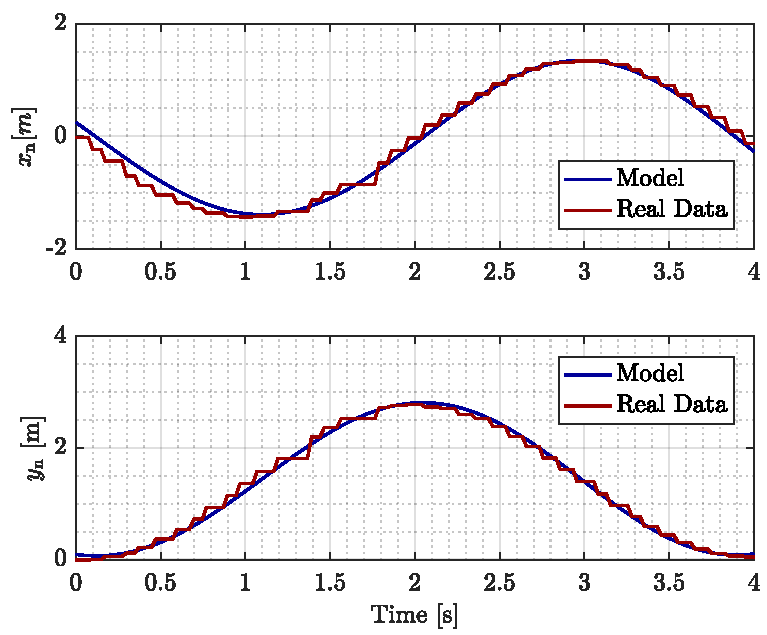
\includegraphics[width=.45\textwidth]{figures/turn_time}
    }
\end{figure}

The results show that the behavior of the real vessel is close to that of the simulated model. It is noticeable that the error between the model and the real behavior is mainly due to the quantization coming from the sampling of the GPS data. Considering this comparison, the model of the vessel is deemed sufficient both for simulation and control design purposes. 

{\vspace*{\fill}
\textit{In Part I, the concept and possible applications of ASVs have been introduced with focus on the design of a control system. The possible implications in the design  performing bathymetric measurements have also been considered. In order to characterize the system at hand, the vessel and its components have been described and the vessels behavior has been represented by means of a mathematical model, which constitutes the basis of the control design.}}



   

    %%% PART 2 %%%
    \part{Design \& Implementation}
    %---------- Chapter 5 ---------------------------------------- Design Approach
    \chapter{Design Approach} \label{chap:designaproach}
%%%%%%Intoduction/description
Based on the requirements mentioned in Section \ref{sec:requirements} the approach shown in \autoref{fig:controllerDiagram} can be designed to autonomously survey an area specified by some coordinates.
\begin{figure}[H]
    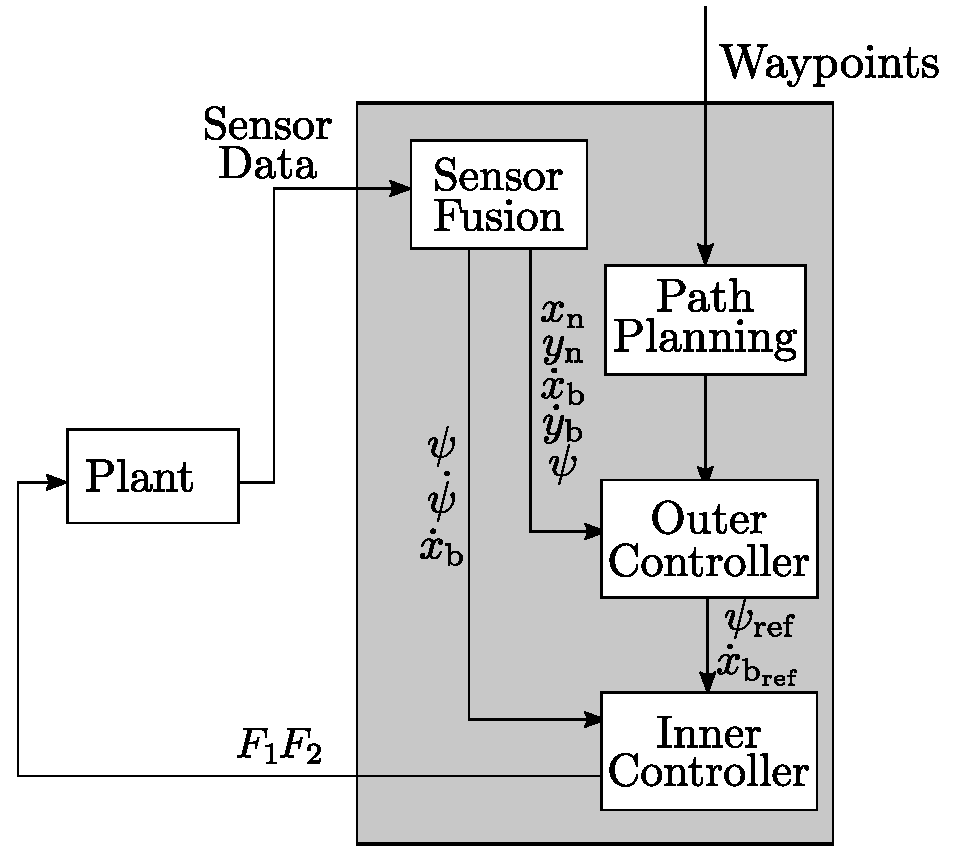
\includegraphics[width=0.3\textwidth]{figures/controllerDiagram2}
    \caption{Diagram of the control approach.}
    \label{fig:controllerDiagram}
\end{figure}
This is achieved by computing a path within the specified area, that preforms a sweeping motion with a predefined width. The path is used as input into the controllers, making the vessel follow it. 

%%%%% Path generation
The control design consists of two controllers, an inner controller and an outer controller. 

As shown on \autoref{fig:controllerDiagram} the outer controller is in charge of following the path by changing the reference of the inner controller to obtain its desired position. Using $x_\mathrm{n}$ , $y_\mathrm{n}$ $x_\mathrm{b}$ $y_b$ and $\psi$ it is able to compute the $\psi_\mathrm{ref}$ and $x_\mathrm{ref}$ needed to follow the path. 

The inner controller uses this references to control $\dot{x}_\mathrm{b}$ and $\dot{\psi}$ by asking for the appropriate $F_{1}$ and $F_{2}$ commands. Two design approaches are tested for the inner controller, an $H_{\infty}$ Controller and a Linear Quadratic Regulator.

The $H_{\infty}$ Controller is designed to be robust towards wind and wave disturbances and towards model errors. The LQR controller, on the other side, is designed to reduce the energy consumption of the vessel as well as to drive the states to the reference values as fast as possible. 
The two approaches for the inner controller are then tested in simulation, to compare the robustness and performance of both of them. \fxnote{Make sure this is correct}

%%%%%Sensor Fusion%%%%%%
Additionally, to improve the precision of the measurements, the sensor data is fused together before it is used as input for the controllers. Two Kalman filters, one for the attitude and another one for the translational behavior are used to filter the measurements, which are based on the model of the vessel. 
 
The filter fuses then the measured sensor data into $\psi$, $x_{b}$, $y_{b}$, $\dot{x}_{b}$ and $\dot{y}_{b}$ which are the states used by the controllers. 

In \autoref{chap:innercontrol} the inner controller design is included while the outer control is described in \autoref{chap:outerController}. The sensor fusion is then presented in \autoref{chap:sensorFusion}.


    %---------- Chapter 7 ---------------------------------------- Controller Design
    \chapter{Controller Design}

Header of control chapter

\begin{figure}[H]
    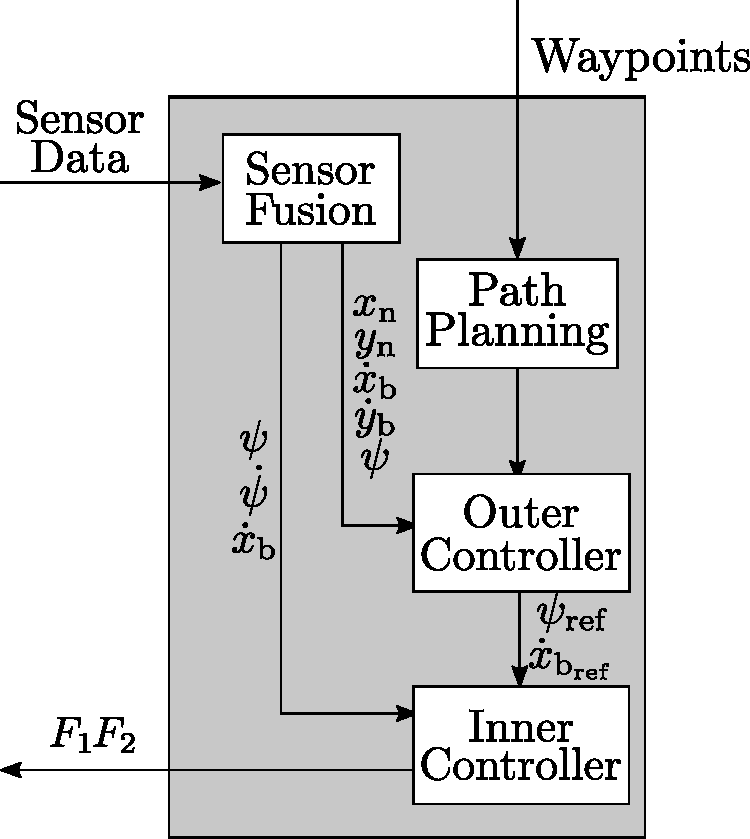
\includegraphics[width=0.8\textwidth]{figures/controllerDiagram}
    \caption{}
    \label{fig:controllerDiagram}
\end{figure}
    \section{Linear Quadratic Regulator} \label{sec:lqr}
The first design approach for the inner controller is a state feedback. The compensator gain is obtained using a Linear Quadratic Regulator (LQR). First, a state space model of the system is created based on the equations derived in \autoref{chap:model}. Then, a cost function based on the state errors and the input usage is minimized in order to calculate the controller gains. 

\subsection{State Space Model}
The linearized model derived in \autoref{sec:linearizationModel}, consisting of \autoref{eq:x_pos_model_lin} to \ref{eq:psi_model_lin}, needs to be represented in state space form in order to design a state space controller. In order to do that, the 3 degree of freedom model used for the control of the vessel is represented as
\begin{flalign}
    \vec{\dot{x}}(t) &= \vec{A} \vec{x}(t) + \vec{B} \vec{u}(t)
    \label{xDotLinear} \\
    \vec{y}(t) &= \vec{C} \vec{x}(t) + \vec{D} \vec{u}(t)
    \label{yLinear} 
\end{flalign}
\begin{where}
    \va{\vec{x}}{is the state vector}{}
    \va{\vec{u}}{is the input vector}{}
    \va{\vec{y}}{is the output vector}{}
    \va{\vec{A}}{is the state matrix}{}
    \va{\vec{B}}{is the input matrix}{}
    \va{\vec{C}}{is the output matrix}{}
    \va{\vec{D}}{is the feed-forward matrix}{}
\end{where}

The state vector is constituted by the angle and velocity in yaw as well as the velocity in x in the body frame. The outputs of the system are yaw angle and velocity in x in the body frame. The input to the system is composed of the two forces applied in the body frame.
%It is important to notice that the position of the vessel in the body reference frame represents the  integration of the velocity along the body frame directions.
%This can also be seen as the position of the vessel with respect to a frame whose origin coincides with that of the NED frame and whose orientation coincides with that of the body frame \cite[p. 173]{TFossen}. 

\begin{minipage}{0.32\linewidth}
    \begin{flalign}
        \vec{x(t)} = 
        \begin{bmatrix}
            \psi\\
            \dot{\psi}\\
            \dot{x}_{b} \\
        \end{bmatrix} \nonumber
        \label{xVector}
    \end{flalign}  
\end{minipage}\hfill
%\hspace{0.03\linewidth}
\begin{minipage}{0.32\linewidth}
    \begin{flalign}
        \vec{y(t)} = 
        \begin{bmatrix}
            \phi \\
            \dot{x}_{b} \\
        \end{bmatrix} \nonumber
        \label{yVector}
    \end{flalign}
\end{minipage}\hfill
%\hspace{0.03\linewidth}
\begin{minipage}{0.32\linewidth}
    \begin{flalign}
        \vec{u(t)}= 
        \begin{bmatrix}
            F_1 \\
            F_2 
        \end{bmatrix}
        \label{uVector}
    \end{flalign} \nonumber
\end{minipage}\hfill

The resulting $\vec{A}$, $\vec{B}$, $\vec{C}$ and $\vec{D}$ matrices are
\begin{flalign}
    \vec{A} &=
    \begin{bmatrix}
        \ 0 & 1                   & 0                \ \ \ \\ 
        \ 0 & -\frac{d_\psi}{I_z} & 0                \ \ \ \\ 
        \ 0 & 0                   & -\frac{d_x}{m_x} \ \ \     
    \end{bmatrix}\rule{30px}{0px}
    \vec{B} = 
    \begin{bmatrix}
        \ 0               & 0                \ \ \ \\
        \ \frac{l_1}{I_z} & -\frac{l_2}{I_z} \ \ \ \\   
        \ \frac{1}{m_x}   & \frac{1}{m_x}    \ \ \
    \end{bmatrix}\rule{30px}{0px}
    \vec{C} =   
    \begin{bmatrix}
        \ 1 & 0 & 0  \ \ \ \\ 
        \ 0 & 0 & 1  \ \ \    
    \end{bmatrix}
    \label{eqStateSpaceABC}
\end{flalign}
and the $\vec{D}$ matrix is zero.

\subsection{Controller Design}
As the controller eventually must be implemented the design is carried out in the discrete domain. To do so, it is necessary to discretize the system. A discrete state space model can be expressed as,
%
\begin{flalign}
  \vec{x}(k+1) &= \vec{A_z} \vec{x}(k) + \vec{B_z} \vec{u}(k)
  \label{xDotLinearDiscrete} \\
  \vec{y}(k)   &= \vec{C_z} \vec{x}(k) + \vec{D_z} \vec{u}(k) \ \ ,
  \label{yLinearDiscrete} 
\end{flalign}
%
where the z subindexes indicate the matrices being in the discrete domain and k is the sample index. The model is discretized using zero order hold. In \autoref{fig:discreteSSBlock} the discrete system is shown in a block diagram. The feed forward matrix is excluded as it is not present in this system.
%
\begin{figure}[H]
  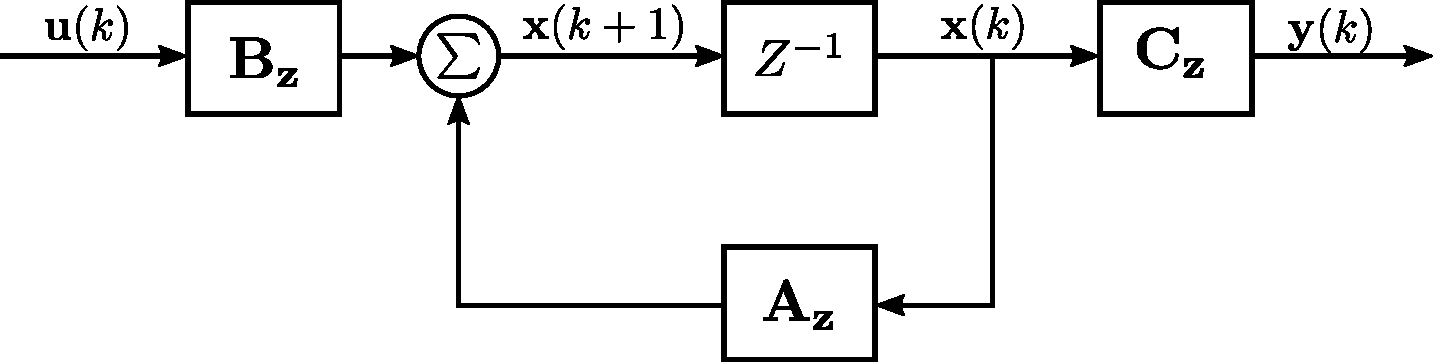
\includegraphics[width=0.6\textwidth]{figures/discreteSystemBlockDiagram}
  \caption{Block diagram of the discrete system without feed forward.}
  \label{fig:discreteSSBlock}
\end{figure}
%
In order to track a reference and handle input disturbances, it is chosen to also include an integral controller in the design. The final control structure is seen in \autoref{fig:blockConrolDesignLQR}.
%
\begin{figure}[H]
  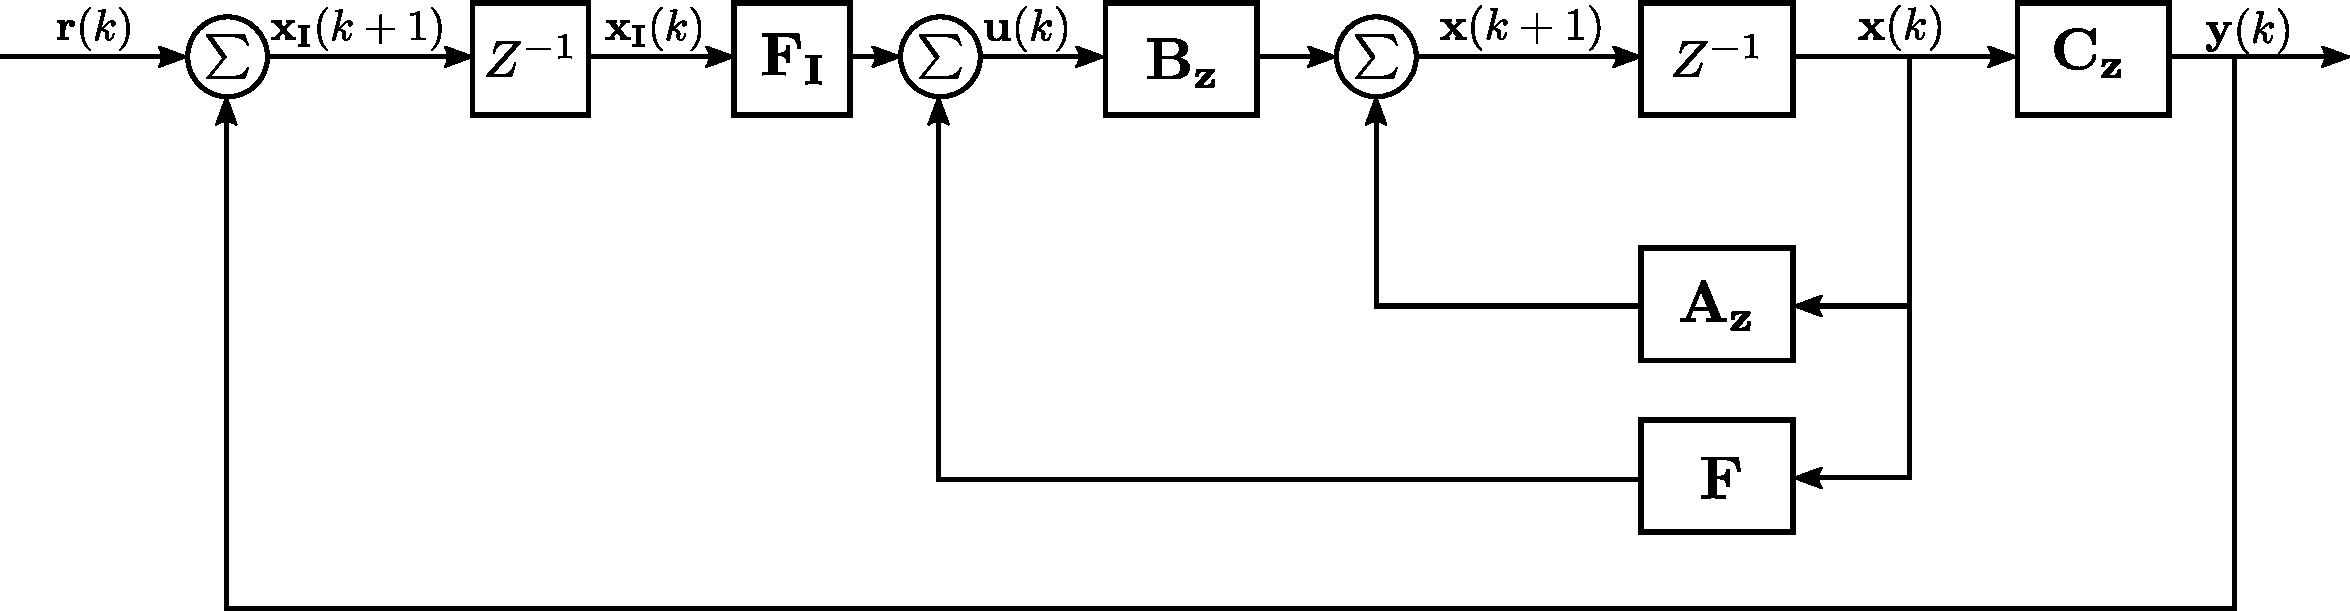
\includegraphics[width=0.9\textwidth]{figures/integralControlBlockDiagram}
  \caption{Block diagram of the control structure in the discrete domain.}
  \label{fig:blockConrolDesignLQR}
\end{figure}
%
To design this feedback system, it is convenient to express it on the following form:
\begin{flalign}
  \vec{x_e}(k+1) &= \vec{A_e} \vec{x}(k) + \vec{B_e} \vec{u}(k) + \vec{r}(k)
  \label{eq:xDotLinearDiscrete} \\
  \vec{y}(k)     &= \vec{C_e} \vec{x}(k)  \ \ .
  \label{eq:yLinearDiscrete} 
\end{flalign}
%
To describe the control design in this form, the $\vec{A_e}$, $\vec{B_e}$ and $\vec{C_e}$ matrices must be constructed. From \autoref{fig:blockConrolDesignLQR}, the discrete state space model for the integral is derived and shown in \autoref{eq:xIDiscrete}.
%
\begin{flalign}
  \vec{x_I}(k+1) &= \vec{x_I}(k) + \vec{y}(k) + \vec{r}(k) \label{eq:xIDiscrete1}  \\
  \vec{x_I}(k+1) &= \vec{x_I}(k) - C_z \vec{x}(k) + \vec{r}(k)  \ \ .
  \label{eq:xIDiscrete}
\end{flalign}
%
This leads to the discrete state space model extended with the integral states expressed as
%
\begin{flalign}
  \begin{bmatrix}
    \vec{x}(k+1)  \\
    \vec{x_I}(k+1)
  \end{bmatrix}
  =
  \begin{bmatrix}
    \vec{A}_{\vec{z}_{3x3}} & \vec{O}_{_{3x2}} \\
   -\vec{C}_{\vec{z}_{2x3}} & \vec{I}_{_{2x2}} \\
  \end{bmatrix}
  \begin{bmatrix}
    \vec{x}(k)    \\
    \vec{x_I}(k)
  \end{bmatrix}
  +
  \begin{bmatrix}
    \vec{B}_{\vec{z}_{3x2}} \\
    \vec{O}_{2x2}
  \end{bmatrix}
  \vec{u}(k)
  +
  \begin{bmatrix}
    \vec{O}_{3x2} \\
    \vec{I}_{2x2}
  \end{bmatrix}
  \vec{r}(k)
  \label{eq:discreteSSWithIntegralX}
\end{flalign}  
%
\begin{flalign}
  \vec{y}(k)
  =
  \begin{bmatrix}
    \vec{C}_{\vec{z}_{2x3}} &  \vec{O}_{2x2}
  \end{bmatrix}
  \begin{bmatrix}
    \vec{x}(k)    \\
    \vec{x_I}(k)
  \end{bmatrix}  \ \ ,
  \label{eq:discreteSSWithIntegralY}
\end{flalign}  
%
which corresponds to \autoref{eq:xDotLinearDiscrete} and \ref{eq:yLinearDiscrete}.

A discrete time infinite horizon LQR is used in the design of the feedback, $\vec{F_e} = [\ \vec{F} \ \ \vec{F}_\mathrm{I} ]\ $, which works by minimizing the cost function,
%
\begin{flalign}
  J = \sum_{k=0}^\infty \vec{x}_k^\mathrm{T}\vec{Q_d}\vec{x}_k + \vec{u}_k^\mathrm{T}\vec{R_d}\vec{u}_k  \ \ .
\end{flalign}
\begin{where}
	\va{\vec{Q_d}}{is the discrete time symmetric positive semidefinite state cost matrix}{}
  \va{\vec{R_d}}{is the discrete time symmetric positive definite input cost matrix}{}
\end{where}

The $\vec{Q_d}$ matrix contains the penalties for the states, such that a higher cost is generated for more critical states, thus driving these states faster to zero. The $\vec{R_d}$ matrix contains the penalties for the inputs. This helps to ensure the inputs are not driven towards saturation.

It is necessary for all states to be stable and controllable. Otherwise the the performance index, $J$, will become infinite \cite[p. 125]{DSNaidu}.\\
The controllability is determined by
%
\begin{flalign}
  \vec{{\mathcal C}}
  = 
  \begin{bmatrix}
    \vec{B}_\mathrm{e} & \vec{A}_\mathrm{e}\vec{B}_\mathrm{e} & \vec{A}_\mathrm{e}^{2} \vec{B}_\mathrm{e} & \vec{A}^{3}_\mathrm{e} \vec{B}_\mathrm{e} & \vec{A}^{4}_\mathrm{e} \vec{B}_\mathrm{e}
  \end{bmatrix}  \ \ ,
  \label{eq:integralControllability}
\end{flalign}
%
of which the rank is 5, that is, the controllability matrix, $\vec{{\mathcal C}}$, has full rank, thus the system is controllable \cite[p. 169]{CTChen}.\\
The eigenvalues of $\vec{A}_\mathrm{e}$ are all on or within the unit-circle in the z-plane, thus, no states are unstable and the LQR design is feasible.

The design approach taken to describe the cost function, $J$, is done by defining weights on the states and inputs for the continuous time infinite horizon LQR cost function,
%
\begin{flalign}
  J_{cont} = \int_{0}^\infty \vec{x}_k^\mathrm{T}\vec{Q}\vec{x}_k + \vec{u}_k^\mathrm{T}\vec{R}\vec{u}_k \  dt\ \ .
  \label{eq:contLQRcost}
\end{flalign}
\begin{where}
  \va{\vec{Q}}{is the continuous time symmetric positive semidefinite state cost matrix}{}
  \va{\vec{R}}{is the continuous time symmetric positive definite input cost matrix}{}
\end{where}

Bryson's rule is used as an initial design method to determine sensible values for the state and input penalties of the $\vec{Q}$ and $\vec{R}$ matrices, as described in \autoref{eq:QRBryson}\\
%
\begin{flalign} 
  Q_{ii} &= \frac{1}{x_{i_\mathrm{max}}\text{}^2} \rule{30px}{0px} R_{ii} = \frac{1}{u_{i_\mathrm{max}} \text{}^2}
  \label{eq:QRBryson}
\end{flalign}
\begin{where}
  \va{x_{i_\mathrm{max}}}{are the maximum acceptable state values}{}
  \va{u_{i_\mathrm{max}}}{are the maximum acceptable input values}{}
\end{where}

The requirements stated in \autoref{sec:requirements} must be taken into account when determining the values of $x_{i_\mathrm{max}}$ and $u_{i_\mathrm{max}}$. As the USV needs a high accuracy for bathymetric measurements, the weights of $\vec{Q}$ are set higher than $\vec{R}$ to ensure priority is focused on driving the states down to zero. The individual integral states are penalized higher than the system states to set further importance on driving the integral states to zero. This will ensure the reference signals are closely tracked. The low weights for $\vec{R}$ also ensures the actuators are not overexerted. This means the actuators will not be driven to saturation and will be used less. This is also ideal for the mobile vessel as the actuators will use less energy, thus the USV will be able to perform longer surveys.

These $\vec{Q}$ and $\vec{R}$ matrices must be discretized, as the state feedback design is done in the discrete time domain. \\
With
%
\begin{flalign}
  \vec{\Phi}(\tau) = e^{\vec{A}\tau} \\
  \vec{\Gamma}(\tau) = \int_{0}^{\tau}e^{\vec{A}\eta}\vec{B}d\eta
\end{flalign}
%
the weighting matrices, $\vec{Q}$ and $\vec{R}$, are discretized using \cite{lqrd}
\begin{flalign}
  \begin{bmatrix}
    \vec{Q_d} & 0 \\
    0 & \vec{R_d} 
  \end{bmatrix}
  = \int_{0}^{T_s}
  \begin{bmatrix}
    \vec{\Phi}^T(\tau)      & 0 \\
    \vec{\Gamma}^T(\tau)    & I
  \end{bmatrix}
  \begin{bmatrix}
    \vec{Q} & 0 \\
    0 & \vec{R}
  \end{bmatrix}
  \begin{bmatrix}
    \vec{\Phi}(\tau)  &   \vec{\Gamma}(\tau) \\
    0           &   I
  \end{bmatrix}
  d\tau
\end{flalign}
%The chosen values for Q and R are shown in \autoref{eq:QRMatrices}.
%
% 
% \begin{flalign}
%   \vec{Q} = 
%   \begin{bmatrix}
%     100 & 0   & 0   & 0   & 0             \\
%     0   & 100 & 0   & 0   & 0             \\
%     0   & 0   & 100 & 0   & 0             \\
%     0   & 0   & 0   & 400 & 0             \\
%     0   & 0   & 0   & 0   & 400
%   \end{bmatrix} \rule{30px}{0px}
%   \vec{R} = 
%   \begin{bmatrix}
%     25\times10^{-6}   & 0                 \\
%     0                 & 25\times10^{-6}
%   \end{bmatrix}
%   \label{eq:QRMatrices}
% \end{flalign}
%
From this the state feedback is calculated by \cite[p. 42]{JLNy},
%
\begin{flalign}
  \vec{F}_\mathrm{e} &= -(\vec{B}_\mathrm{e}^\mathrm{T} \vec{P}\vec{B}_\mathrm{e} + \vec{R_d})^{-1}  \vec{B}_\mathrm{e}^\mathrm{T} \vec{P}\vec{A}_\mathrm{e} \ \ ,
  \label{eq:QRFeedback}
\end{flalign}
%
where $\vec{P}$ can be found as the solution of the infinite horizon algebraic discrete-time Riccati equation \cite[p. 42]{JLNy},
%
\begin{flalign}
\vec{P} &= \vec{A}_\mathrm{e}^\mathrm{T} \vec{P} \vec{A}_\mathrm{e} + \vec{Q_d} - \vec{A}_\mathrm{e}^\mathrm{T} \vec{P} \vec{B}_\mathrm{e} (\vec{B}_\mathrm{e}^\mathrm{T} \vec{P} \vec{B}_\mathrm{e} + \vec{R_d})^{-1} \vec{B}_\mathrm{e}^\mathrm{T} \vec{P} \vec{A}_\mathrm{e} \ \ .
\label{eq:discreteInfRiccati}
\end{flalign}
%
Once $\vec{F}_\mathrm{e}$ is obtained, it is split into the two feedback matrices, $\vec{F}_\mathrm{e} = [\ \vec{F} \ \ \vec{F}_\mathrm{I}\ ]$, and implemented, following the control structure provided in \autoref{fig:blockConrolDesignLQR}.

These design has been simulated together with the nonlinear model of the system. Its performance is also compared to the $\mathcal{H}_\infty$ controller designed in \autoref{sec:Hinf} when disturbances, measurement noise and parameter uncertainties are present. The simulations are presented in \autoref{sec:comparison}.










    \section{$\mathcal{H}_\infty$ Design}
The linearized model in \autoref{sec:linearizationModel} has varying parameters, such as the added mass and damping coefficients. The vessel may also experience external disturbances, such as wind forces. During surveying, the vessel needs to be robust to these model variations and it must be able to sufficiently reject disturbances. Using the $\mathcal{H}_\infty$ design technique, a robust controller for the vessel can be synthesized. The design of such controller differs from the LQR design. In this case, the design of model and controller is done simultaneously and can not be clearly separated as for the LQR case.

The $\mathcal{H}_\infty$ problem consists of finding an internally stabilizing controller that provides a closed loop $\mathcal{H}_\infty$ norm less than some bound $\gamma$ \cite[p. 835]{JCDoyle}, \cite[pp. 92-93]{AAStoorvogel}. Such controller is also called suboptimal $\mathcal{H}_\infty$ controller, as there might be smaller $\gamma$ yielding an internally stabilizing controller.% The reason for not deigning the optimal controller is \fxnote{write reason}

A more detailed mathematical formulation of the $\mathcal{H}_\infty$ problem and its solution is given in \cite[pp. 91-119]{AAStoorvogel}. 

The state space model from \autoref{xDotLinear} and \autoref{yLinear} needs to be remodeled into a state space form suitable for solving the suboptimal $\mathcal{H}_\infty$ control problem. This representation starts with the equations
For solving the suboptimal $\mathcal{H}_\infty$ control problem, the system has to be expressed in a particular state space form \cite[pp. 95]{AAStoorvogel}, \cite[p. 64]{RobustNotes}. This form is
\begin{flalign}
  \vec{\dot{x}}(t) &= \vec{A}_1 \vec{x}(t) + \vec{B}_1 \vec{w}(t) + \vec{B}_2 \vec{u}(t)\ ,
  \label{eq:xDotHinf} \\
  \vec{z}(t) &= \vec{C}_1 \vec{x}(t) + \vec{D}_{11} \vec{w}(t) + \vec{D}_{12} \vec{u}(t)\ ,
  \label{eq:zHinf} \\
  \vec{y}(t) &= \vec{C}_2 \vec{x}(t) + \vec{D}_{21} \vec{w}(t) + \vec{D}_{22} \vec{u}(t)\ ,
  \label{eq:yHinf} 
\end{flalign}
\begin{where}
  \va{\vec{x}}{is the state vector}{}
  \va{\vec{w}}{is the uncontrolled input vector}{}
  \va{\vec{u}}{is the controlled input vector}{}
  \va{\vec{z}}{is the performance output vector}{}
  \va{\vec{y}}{is the measured output vector}{}
  \va{\vec{A}_1}{is the state matrix}{}
  \va{\vec{B}_1}{is the uncontrolled input matrix}{}
  \va{\vec{B}_2}{is the controlled input matrix}{}
  \va{\vec{C}_1}{is the performance output matrix}{}
  \va{\vec{D}_{11}}{is the direct feedthrough matrix from $\vec{w}$ to $\vec{z}$}{}
  \va{\vec{D}_{12}}{is the direct feedthrough matrix from $\vec{u}$ to $\vec{z}$}{}
  \va{\vec{C}_2}{is the measured output matrix}{}
  \va{\vec{D}_{21}}{is the direct feedthrough matrix from $\vec{w}$ to $\vec{y}$}{}
  \va{\vec{D}_{22}}{is the direct feedthrough matrix from $\vec{u}$ to $\vec{y}$}{}
\end{where}

The $\mathcal{H}_\infty$ model representation can also be seen in \autoref{fig:HinfDiag}, where all signals and matrices involved in the design process are represented.
\begin{figure}[H]
	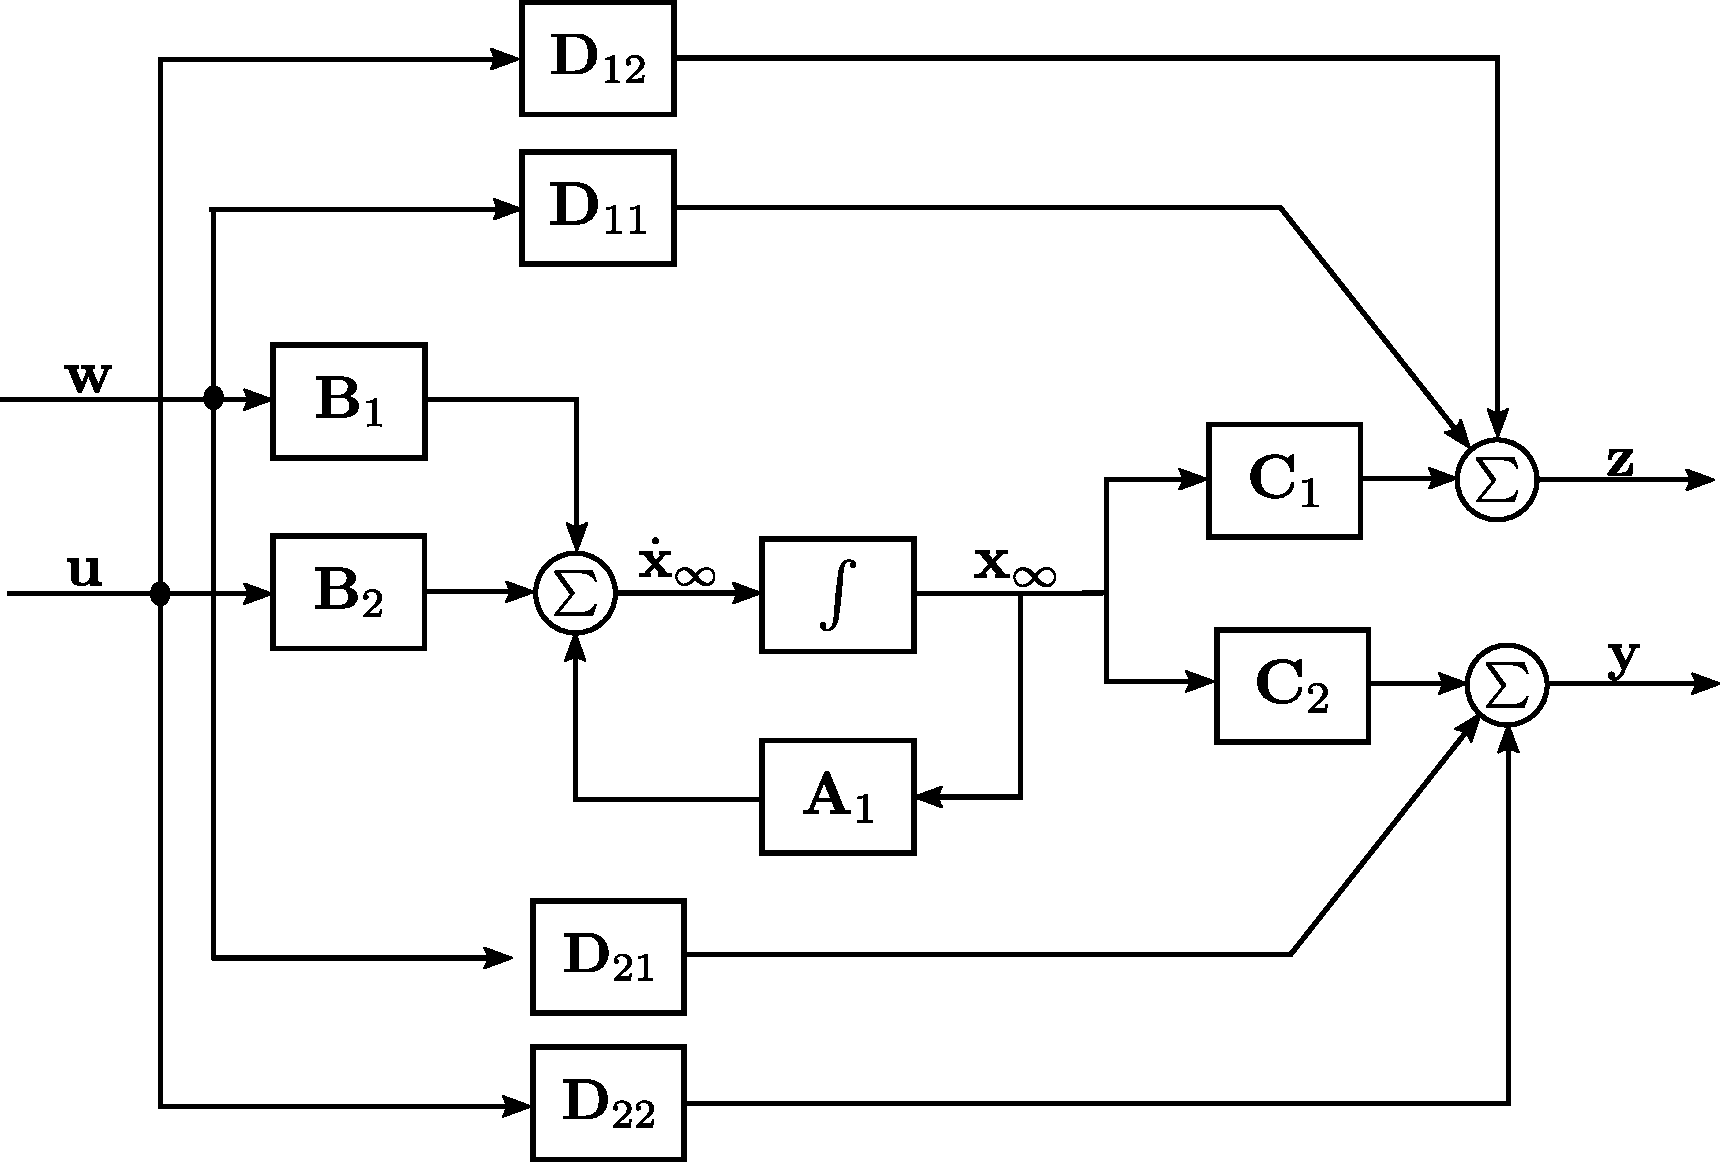
\includegraphics[width=0.6\textwidth]{figures/HinfDiag}
	\caption{Block diagram used in the $\mathcal{H}_\infty$ controller design.}
	\label{fig:HinfDiag}
\end{figure}

The method used to achieve the solution to the problem requires assuming certain conditions on the matrix in the model \cite[p. 835]{JCDoyle}. These conditions are 
\begin{itemize}
	\item $\left (\vec{A}_1,\vec{B}_1 \right)$ and $\left( \vec{A}_1, \vec{B}_2 \right)$ are stabilizable.
	\item $\left (\vec{C}_1,\vec{A}_1 \right)$ and $\left( \vec{C}_2, \vec{A}_1 \right)$ are detectable.
	\item $\vec{D}_{12}^\mathrm{T}[\vec{C}_1\ \vec{D_{12}}]$ is $[\vec{0}\ \vec{I}]$.
	\item $	\begin{bmatrix}
				\vec{B}_1 \\
				\vec{D}_{21} 
			\end{bmatrix}\vec{D}_{21}^\mathrm{T}$ is $[\vec{0}\ \vec{I}]$.
	\item $\vec{D}_{11}$ and $\vec{D}_{22}$ are zero.
\end{itemize}

For obtaining the matrices present in \autoref{eq:xDotHinf}, \ref{eq:zHinf} and \ref{eq:yHinf}, the content of the state vector and signal vectors needs to be defined.

\subsection*{State Vector}
The state vector construction starts with the three states that define the basic dynamics of the system. Namely, $\psi$, $\dot{\psi}$ and $\dot{x}_\mathrm{b}$. As some reference tracking is desired, integral states need to be included in the state vector, these depend on the measured output and the reference signal as 
\begin{flalign}
	\vec{\dot{x}}_\mathrm{int} =
	\begin{bmatrix}
		x_{int_{\psi}} \\
		x_{int_{\dot{x}_\mathrm{b}}}
	\end{bmatrix}\ = 
	\begin{bmatrix}
		\psi_\mathrm{ref}-\psi \\
		\dot{x}_\mathrm{b,ref} - \dot{x}_\mathrm{b}
	\end{bmatrix}\ .
	\label{eq:xintVectorHinf}
\end{flalign}

The state vector also includes the states coming from the reference, disturbance and noise models. These extra states, not only show the dynamics of the uncontrolled inputs, but also reflect the weighting functions that have been applied to each of them. This process is carried out in order to modify how the uncontrolled inputs affect the states, this is normally done through transfer functions, \cite{MSalari}. In order to include weights in the state space representation, some states for each uncontrolled input need to be defined. \autoref{fig:WeightDiag} shows an example of how an uncontrolled input is weighted so it can be included in the state space representation.
\begin{figure}[H]
	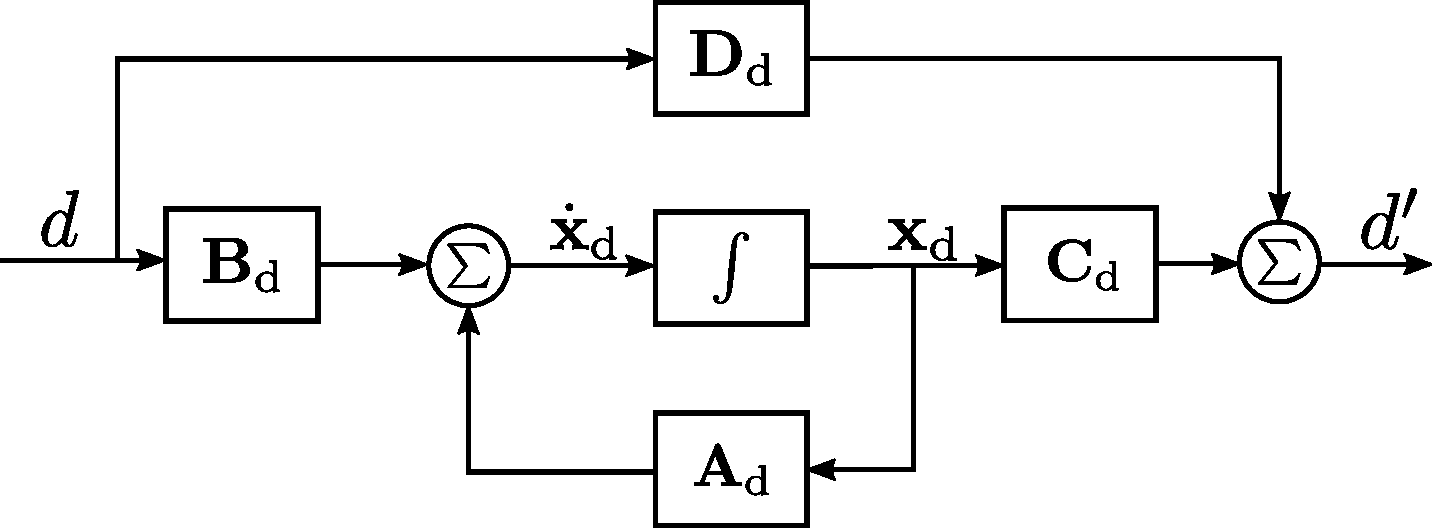
\includegraphics[width=0.6\textwidth]{figures/WeightDiag}
	\caption{Block diagram illustrating how an uncontrolled input is weighted in the $\mathcal{H}_\infty$ controller design. $d$ is the uncontrolled input and $d'$ is the weighted uncontrolled input. The states $\vec{x}_\mathrm{d}$ are included in the state vector of the $\mathcal{H}_\infty$ state space representation.}
	\label{fig:WeightDiag}
\end{figure}
The uncontrolled input states are part of the state vector. The $\vec{A}_\mathrm{d}$, $\vec{B}_\mathrm{d}$, $\vec{C}_\mathrm{d}$ and $\vec{D}_\mathrm{d}$ in \autoref{fig:WeightDiag} can be calculated from a weighting function as in the example given in \autoref{eq:weightingexampleLP}, where the uncontrolled input $d$ is weighted by means of a first order transfer function with low-pass characteristics.
\begin{flalign}
	\frac{d'}{d}=\frac{a}{s+a} \rightarrow \dot{d}' = -a d' + a d \rightarrow \begin{cases} \dot{x}_\mathrm{d} = -a x_\mathrm{d} + a d \\ d' = x_\mathrm{d} \end{cases}\label{eq:weightingexampleLP} 
\end{flalign}
\begin{where}
	\va{a}{is a parameter defining the pole position of the weighting function}{}
\end{where}
Another example with a high pass weighting function is shown in \autoref{eq:weightingexampleHP}.
\begin{flalign}
	\frac{n'}{n}=\frac{s}{s+a} = \frac{-a}{s+a}-1 \rightarrow \begin{cases} \dot{x}_\mathrm{n} = -a x_\mathrm{n} + n \\ n' = - a x_\mathrm{n} + n  \end{cases}\label{eq:weightingexampleHP} 
\end{flalign}

This process also entails defining the weights for each uncontrolled input. The weight on the reference is set to be a first order transfer function with a very fast pole so the step input does not get distorted. The weights on the input disturbances are also low pass filtered as most of them appear at low frequencies. The noise, on the other hand, is weighted according to a high pass filter, as it is stronger in the high frequency range. In this way, the controller design focuses on achieving a robust controller with respect to the uncontrolled inputs in their particular frequency ranges. The weights for each uncontrolled input are are
\fxnote{include proper weighting transfer functions and it looks a bit ugly as it is now}
\begin{flalign}
	W_{\psi_\mathrm{ref}} &= \frac{1}{s+1}\ ,\  W_{\dot{x}_\mathrm{b,ref}} = \frac{1}{s+1}\ ,\nonumber \\
	W_{F_\mathrm{wind}} &= \frac{1}{s+1}\ ,\nonumber\   W_{\tau_\mathrm{wind}} = \frac{1}{s+1}\ , \nonumber\\
	W_{F_\mathrm{wave}} &= \frac{1}{s+1}\ , \nonumber\  W_{\tau_\mathrm{wave}} = \frac{1}{s+1}\ , \nonumber\\
	W_{n_\psi} &= \frac{s}{s+1}\ , \nonumber\ 	W_{n_{\dot{x}_\mathrm{b}}} = \frac{s}{s+1}\ .\nonumber
\end{flalign}}

The states coming from the weighting functions, together with the system states and the integral states, constitute the state vector as 
\begin{flalign}
	\vec{x}(t)=
	\begin{bmatrix}
		\psi & \dot{\psi} & \dot{x}_\mathrm{b} & x_{int_{\psi}} & x_{int_{\dot{x}_\mathrm{b}}} & x_{F_\mathrm{wind}} & x_{\tau_\mathrm{wind}} & x_{F_\mathrm{wave}} & x_{\tau_\mathrm{wave}} & x_{n_{\psi}}\ \ \  x_{n_{\dot{x}_\mathrm{b}}}
	\end{bmatrix}^\mathrm{T}\ .
	\label{eq:xVectorHinf}
\end{flalign}

\subsection*{Controlled Inputs Vector}
The controlled input are the two forces provided by the thrusters of the boat, that is, 
\begin{flalign}
	\vec{u(t)}= 
	\begin{bmatrix}
		F_1 & F_2 
	\end{bmatrix}^\mathrm{T}\ .
	\label{eq:uVectorHinf}
\end{flalign} \nonumber


\subsection*{Uncontrolled Input vector}
The uncontrolled inputs include the references to be tracked, the input disturbances, and the measurement noises. The size of this vector depends on the amount of reference signals, the input disturbances considered (wind, waves) and the amount of measured outputs, as these are normally affected by noise. The references for the inner controller are two, the heading, $\psi$, and the translational speed along the $x_\mathrm{b}$ direction. The input disturbances are coming from wind and from waves. These two elements potentially generate both a force along the $x_\mathrm{b}$ and a torque in $\psi$. The noise vector affects measured outputs considered for the inner controller, which are the outputs, $\psi$ and $\dot{x}_\mathrm{b}$. The uncontrolled input vector is formed as
\begin{flalign}
	\vec{w(t)}= 
	\begin{bmatrix}
		\psi_\mathrm{ref} & \dot{x}_\mathrm{b},_\mathrm{ref} & F_\mathrm{wind} & \tau_\mathrm{wind} & F_\mathrm{wave} & \tau_\mathrm{wave}& n_{\psi} & n_{\dot{x}_\mathrm{b}}
	\end{bmatrix}^\mathrm{T} \ .
	\label{eq:wVectorHinf}
\end{flalign} \nonumber
\begin{where}
	\va{n_\mathrm{x}}{is noise affecting measured output x}{}
	\va{F_\mathrm{wind/wave}}{is the force of the wind/waves along the $x_\mathrm{b}$ direction}{}
	\va{\tau_\mathrm{wind/wave}}{is the torque of the wind/waves in $\psi$}{}
\end{where}

\subsection*{Measurement Output Vector}
The measurement output vector includes the outputs that are to track a reference. It also includes the integral states as they represent the error between the outputs and the references and are affected by noise. Consequently, the output vector contains 4 elements and is represented as 
\begin{flalign}
	\vec{y(t)}= 
	\begin{bmatrix}
		\psi & \dot{x}_\mathrm{b} & \vec{x}_\mathrm{int}
	\end{bmatrix}^\mathrm{T}\ .
	\label{eq:yVectorHinf}
\end{flalign} \nonumber

\subsection*{Performance Output Vector}
The performance output contains all variables whose performance should be taken into account by the controller. As the design entails a state feedback control, all the states are considered performance outputs. The controlled inputs are also part of this vector as it is desired to set some limitations or constant weights in order to account for the saturation of these inputs in the real system.
\begin{flalign}
	\vec{z(t)}= 
	\begin{bmatrix}
		\vec{x} & \vec{u}
	\end{bmatrix}^\mathrm{T}\ .
	\label{eq:zVectorHinf}
\end{flalign} \nonumber

Once the state, input and output vectors have been defined, the model matrices can be derived.

\subsection*{Model Matrices}

The matrices present in \autoref{eq:xDotHinf}, \ref{eq:zHinf} and \ref{eq:yHinf} are derived from the relations between the different signals and states. 

Starting with \autoref{eq:xDotHinf}, it contains the $\vec{A}_1$, $\vec{B}_1$ and $\vec{B}_2$ matrices. 

The matrix $\vec{A}_1$ describes the dynamics of the system states and all the other added states, which account for the references and disturbances. Its value can be seen in \autoref{app:matrices} and its structure is \fxnote{make appendix for all matrices}
\begin{flalign}
	\label{eq:A1}
	\vec{A}_1 &=
	\begin{bmatrix}
		\vec{A} & \vec{0}_{3\mathrm{x}2} & \vec{B}_\mathrm{dist} & \vec{B}_\mathrm{dist} & \vec{0}_{3\mathrm{x}2} \\
		-\vec{C} & \vec{A}_\mathrm{i} & \vec{0}_{2\mathrm{x}2} & \vec{0}_{2\mathrm{x}2} & \vec{0}_{2\mathrm{x}2} \\
		\vec{0}_{2\mathrm{x}3} & \vec{0}_{2\mathrm{x}2} & \vec{A}_\mathrm{wind} & \vec{0}_{2\mathrm{x}2} & \vec{0}_{2\mathrm{x}2} \\
		\vec{0}_{2\mathrm{x}3} & \vec{0}_{2\mathrm{x}2} & \vec{0}_{2\mathrm{x}2} & \vec{A}_\mathrm{wave} & \vec{0}_{2\mathrm{x}2} \\
		\vec{0}_{2\mathrm{x}3} & \vec{0}_{2\mathrm{x}2} & \vec{0}_{2\mathrm{x}2} & \vec{0}_{2\mathrm{x}2} & \vec{A}_\mathrm{noise} 
	\end{bmatrix}\ . \nonumber
\end{flalign}
It can be seen that the matrix is composed by submatrices that correspond to the different parts of the system, namely for the original states in the first three rows, the integral states for reference tracking in the next two rows and the uncontrolled inputs in the last six rows. The last submatrices result from the weighting functions applied to the different uncontrolled inputs.

$\vec{B}_1$ relates the uncontrolled inputs with the state derivatives, its value is shown in \autoref{app:matrices}. Its structure in terms of the different submatrices is \begin{flalign}
	\label{eq:B1}
	\vec{B}_1 &=
	\begin{bmatrix}
		\vec{0}_{3\mathrm{x}2} & \vec{0}_{3\mathrm{x}2} & \vec{0}_{3\mathrm{x}2} & \vec{0}_{3\mathrm{x}2} \\
		\vec{I}_{2\mathrm{x}2} & \vec{0}_{2\mathrm{x}2} & \vec{0}_{2\mathrm{x}2} & \vec{0}_{2\mathrm{x}2} \\
		\vec{0}_{2\mathrm{x}2} & \vec{B}_\mathrm{wind} & \vec{0}_{2\mathrm{x}2} & \vec{0}_{2\mathrm{x}2} \\
		\vec{0}_{2\mathrm{x}2} & \vec{0}_{2\mathrm{x}2} & \vec{B}_\mathrm{wave} & \vec{0}_{2\mathrm{x}2} \\
		\vec{0}_{2\mathrm{x}2} & \vec{0}_{2\mathrm{x}2} & \vec{0}_{2\mathrm{x}2} & \vec{B}_\mathrm{noise} 
	\end{bmatrix}\ . \nonumber
\end{flalign}

The matrix $\vec{B}_2$ relates the controlled inputs to the states, in this case, the motor thrusters only affect the system states. The $\vec{B}_2$ matrix is constructed as 
\fxnote{write the proper B2 matrix}
\begin{flalign}
	\label{eq:B2}
	\vec{B}_2 &=
	\begin{bmatrix}
		\vec{B}\\
		\vec{0}_{2\mathrm{x}2} \\
		\vec{0}_{2\mathrm{x}2} \\
		\vec{0}_{2\mathrm{x}2} \\
		\vec{0}_{2\mathrm{x}2} 
	\end{bmatrix}\ . \nonumber
\end{flalign}

Next, the matrices appearing in \autoref{eq:zHinf} are derived. These are $\vec{C}_1$, $\vec{D}_{11}$ and $\vec{D}_{12}$ and they can be considered to be weighting matrices where the importance of each of the performance outputs and the usage of the controlled inputs can be specified.

The $\vec{C}_1$ matrix relates the states and the performance outputs, it is formed by a diagonal matrix, where some weights are applied to each state, and some zero rows corresponding to the controlled inputs of the system. The matrix is constructed as 
\begin{flalign}
	\label{eq:C1}
	\vec{C}_1 &=
	\begin{bmatrix}
		\vec{W}_\mathrm{x} & \vec{0}_{3\mathrm{x}2} &  \vec{0}_{3\mathrm{x}2} &  \vec{0}_{3\mathrm{x}2}  & \vec{0}_{3\mathrm{x}2} \\
		\vec{0}_{2\mathrm{x}3}  &  \vec{W}_\mathrm{i}  & \vec{0}_{2\mathrm{x}2} &  \vec{0}_{2\mathrm{x}2}  & \vec{0}_{2\mathrm{x}2} \\
		\vec{0}_{2\mathrm{x}3}  & \vec{0}_{2\mathrm{x}2} &  \vec{W}_\mathrm{wind} &  \vec{0}_{2\mathrm{x}2} &  \vec{0}_{2\mathrm{x}2} \\
		\vec{0}_{2\mathrm{x}3} &  \vec{0}_{2\mathrm{x}2}  & \vec{0}_{2\mathrm{x}2}  & \vec{W}_\mathrm{wave}  & \vec{0}_{2\mathrm{x}2} \\
		\vec{0}_{2\mathrm{x}3} &  \vec{0}_{2\mathrm{x}2}  & \vec{0}_{2\mathrm{x}2} &  \vec{0}_{2\mathrm{x}2} &  \vec{W}_\mathrm{noise} \\
		\vec{0}_{2\mathrm{x}3}  & \vec{0}_{2\mathrm{x}2}  & \vec{0}_{2\mathrm{x}2}  & \vec{0}_{2\mathrm{x}2} &  \vec{0}_{2\mathrm{x}2} \\
		\vec{0}_{2\mathrm{x}3}  & \vec{0}_{2\mathrm{x}2}  & \vec{0}_{2\mathrm{x}2}  & \vec{0}_{2\mathrm{x}2}  & \vec{0}_{2\mathrm{x}2} 
	\end{bmatrix}\ . \nonumber
\end{flalign}
Where the weighting submatrices values have been chosen as \fxnote{explain how we choose the weights}.The value of the $\vec{C}_1$ matrix can be seen in \autoref{app:matrices}.

$\vec{D}_{11}$ is a zero matrix as there is no relation between the uncontrolled inputs and the performance outputs in the $\mathcal{H}_\infty$ design. It has as many rows as the number of elements in the performance output and as many columns uncontrolled  inputs.

The $\vec{D}_{12}$ has non-zero elements only in the entries that weight the inputs, its values can be seen in \autoref{app:matrices}. The matrix is constructed as 
\begin{flalign}
	\label{eq:D12}
	\vec{D}_{12} &=
	\begin{bmatrix}
		\vec{0}_{2\mathrm{x}3} \\
		\vec{0}_{2\mathrm{x}2} \\
		\vec{0}_{2\mathrm{x}2} \\
		\vec{0}_{2\mathrm{x}2} \\
		\vec{0}_{2\mathrm{x}2} \\
		\vec{W}_\mathrm{u}
	\end{bmatrix}\ . \nonumber
\end{flalign}

Finally, the matrices present in \autoref{eq:yHinf}, $\vec{C}_2$, $\vec{D}_{12}$ and $\vec{D}_{22}$, are derived below, they are not part of the design as they describe how the measured outputs of the system are affected. 

The $\vec{C}_2$ matrix relates the states with the measured outputs, selecting the $\psi$ and $\dot{x}_\mathrm{b}$ states and the integral states to form the output, as seen in \autoref{eq:C2}. This matrix can also be seen in \autoref{app:matrices}.
\begin{flalign}
	\label{eq:C2}
	\vec{C}_2 &=
	\begin{bmatrix}
		\vec{C} & \vec{0}_{2\mathrm{x}2} & \vec{0}_{2\mathrm{x}2} & \vec{0}_{2\mathrm{x}2} & \vec{C}_\mathrm{noise} \\
		\vec{0}_{2\mathrm{x}3} & \vec{I}_{2\mathrm{x}2} & \vec{0}_{2\mathrm{x}2} & \vec{0}_{2\mathrm{x}2} & \vec{C}_\mathrm{noise} 
	\end{bmatrix}\ . \nonumber
\end{flalign}

The $\vec{D}_{21}$ matrix relates uncontrolled inputs with the measurement outputs, mainly adding the noise to the outputs as
\begin{flalign}
	\label{eq:D21}
	\vec{D}_{21} &=
	\begin{bmatrix}
		\vec{0}_{2\mathrm{x}2} & \vec{0}_{2\mathrm{x}2} & \vec{0}_{2\mathrm{x}2} & \vec{D}_{noise} \\
		\vec{0}_{2\mathrm{x}2} & \vec{0}_{2\mathrm{x}2} & \vec{0}_{2\mathrm{x}2} & \vec{D}_{noise} 
	\end{bmatrix}\ . \nonumber
\end{flalign}
The values for this matrix can be seen in \autoref{app:matrices}.

After setting up the model, which includes part of the controller design, the $\mathcal{H}_\infty$ controller can be found by solving a Riccatti equation defined as
\begin{flalign}
	\label{eq:Xinf}
	\vec{X}_\infty &= Ric
	\begin{bmatrix}
		\vec{A} & \gamma^{-2}\vec{B}_1\vec{B}_1^\mathrm{T} - \vec{B}_2\vec{B}_2^\mathrm{T} \\
		-\vec{C}_1^\mathrm{T}\vec{C}_1 & -\vec{A}^\mathrm{T}
	\end{bmatrix}\ , \nonumber
\end{flalign}

and calculating the state feedback gain matrix as
\begin{flalign}
	\vec{F}_\infty = -\vec{B}_2^\mathrm{T}\vec{X}_\infty
\end{flalign}

The value of $\gamma$ in the Riccatti equation has been chosen according to \fxnote{explain value for gamma}







    \section{Comparison between Controller Designs}\label{sec:comparison}
The two controller designs are now compared in order to analyze the robustness, the performance. The control inputs applied by each controller are also compared. The simulations carried out in this section include input disturbances, both from wind and waves, and measurement noise in the outputs. The measurement noise are model to have a power spectral density similar to the sensor noise that comes out of the sensor fusion. Model perturbations are also included.

The performance comparison is evaluated by looking at the response of the nonlinear model of the system when tracking a step in the reference inputs, $\dot{x}_\mathrm{b,ref}$ and $\psi_\mathrm{ref}$. 

The disturbances applied to the system range from $\pm$\num{1.5} N in the force along the $\dot{x}_\mathrm{b}$ axis and $\pm$\num{1.5} Nm in the torque around the $z_\mathrm{b}$ axis. These disturbances come from wind and waves. The frequency of the latter is also varied from 0 to 10 Hz.

The parameter uncertainties are assumed to vary $\pm$20\% from their nominal value. The parameters varied in the simulation are the added mass, $m_\mathrm{x}$, the moment of inertia around the $z_\mathrm{b}$ axis, $I_\mathrm{z}$, the damping coefficients, $d_\mathrm{x}$ and $d_\psi$, and the lengths where the forces are applied, $l_1$ and $l_2$. 

\autoref{fig:xbdot_mc_lqr} and \ref{fig:xbdot_mc_rob} show the step response of the velocity along the $x_\mathrm{b}$ direction from 1000 simulations where the model parameters and the disturbances were varied randomly within the defined ranges. These simulations also include a reference step in $\psi$ at 10 seconds that causes a perturbation in the $\dot{x}_\mathrm{b}$ response. 
\begin{figure}[H]
    \captionbox 
    {   
        Step response in $x_\mathrm{b}$ of the Linear Quadratic Regulator, where the nominal response, the maximum variation region and the 1-$\sigma$ region are shown.
        \label{fig:xbdot_mc_lqr}
    }                                                                 
    {                                                                  
        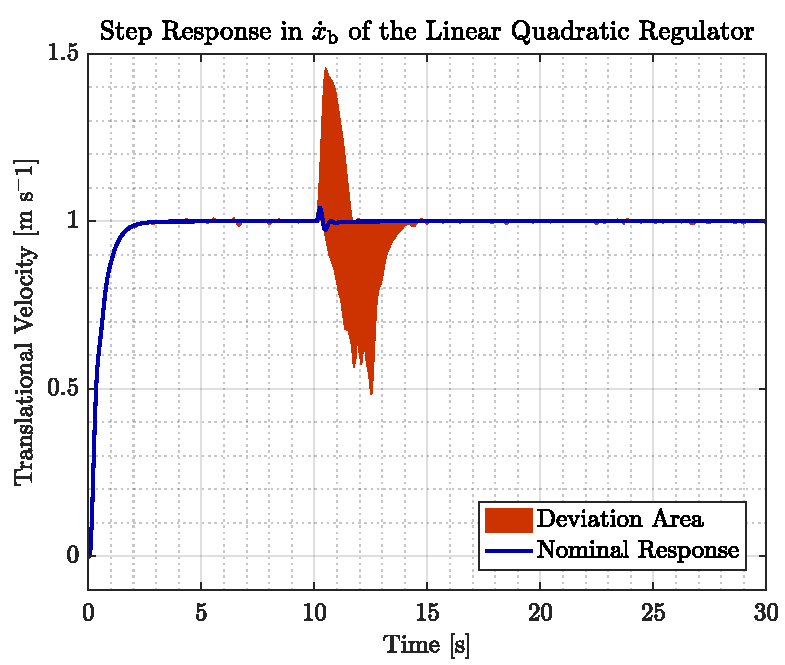
\includegraphics[width=.45\textwidth]{figures/xbdot_mc_lqr}         
    }                                                                    
    \hspace{5pt}                                                          
    \captionbox  
    {      
        Step response in $x_\mathrm{b}$ of the $\mathcal{H}_\infty$ Controller, where the nominal response, the maximum variation region and the 1-$\sigma$ region are shown.
        \label{fig:xbdot_mc_rob}
    }                                                                          
    {
        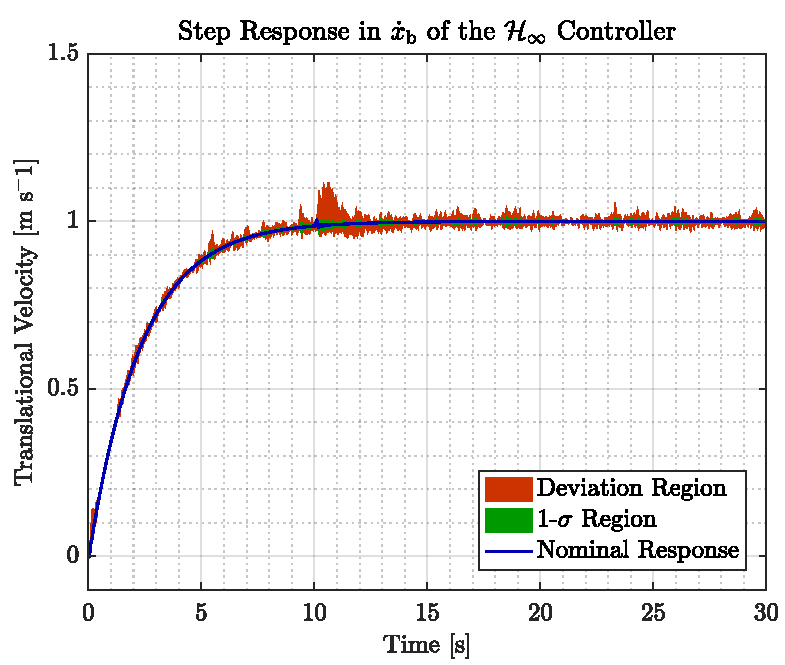
\includegraphics[width=.45\textwidth]{figures/xbdot_mc_rob}
    }
\end{figure}
As it can be seen, both controllers are able to track the given reference in $\dot{x}_\mathrm{b}$. The controller designed using LQR theory yields a fast controller, but the change in reference in the $\psi$ angle leads to a great perturbation in the vessel speed, reaching almost 50\%, while the 1-$\sigma$ values stays below 10\%. There is no steady state error once the perturbation has been compensated by the controller. The $\mathcal{H}_\infty$ Controller on the other hand, is much slower in terms of settling time, the perturbation introduced when changing $\psi_\mathrm{ref}$ has a 1-$\sigma$ value that is almost zero and a maximum value around 10\%. This is acceptable as the forward velocity of the boat does not require a fast response and it is not a critical parameter for he outer controller.

In \autoref{fig:xbdot_mc_lqr_error} and \ref{fig:xbdot_mc_rob_error}, a closed look to the difference of the step responses with respect to the nominal behavior is shown.
\begin{figure}[H]
    \captionbox 
    {   
        Difference with the nominal behavior in $x_\mathrm{b}$ of the Linear Quadratic Regulator, where the maximum variation region and the 1-$\sigma$ region are shown.
        \label{fig:xbdot_mc_lqr_error}
    }                                                                 
    {                                                                  
        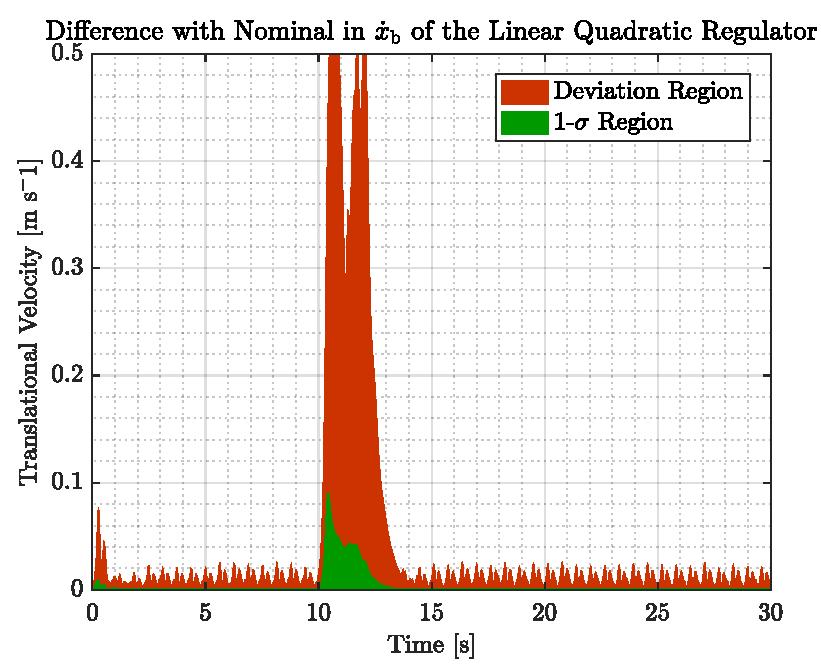
\includegraphics[width=.45\textwidth]{figures/xbdot_mc_lqr_error}         
    }                                                                    
    \hspace{5pt}                                                          
    \captionbox  
    {      
         Difference with the nominal behavior in $x_\mathrm{b}$ of the $\mathcal{H}_\infty$ Controller, where the maximum variation region and the 1-$\sigma$ region are shown.
        \label{fig:xbdot_mc_rob_error}
    }                                                                          
    {
        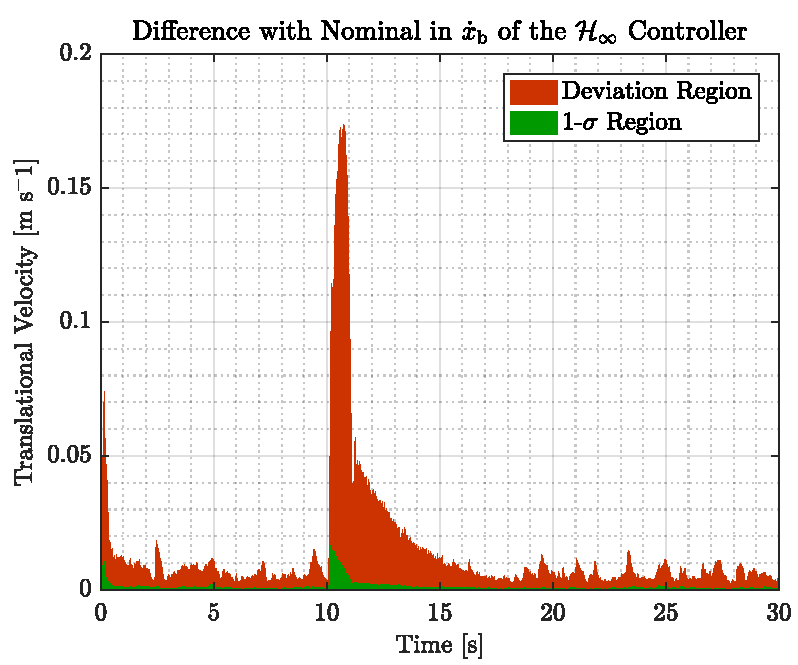
\includegraphics[width=.45\textwidth]{figures/xbdot_mc_rob_error}
    }
\end{figure}

It can be seen that the error keeps at a low value until the step for $\psi$ is applied, and the highest disturbance occurs, being the $\mathcal{H}_\infty$ Controller the one that is able to reject better the disturbance and the one with less variation from the nominal performance.

In \autoref{fig:yaw_mc_lqr} and \ref{fig:yaw_mc_rob}, the performance of the controllers in analyzed by looking at the step response when tracking a reference in $\psi$. These plots are part of the same simulations depicted in \autoref{fig:xbdot_mc_lqr} and \ref{fig:xbdot_mc_rob}, and therefore cope with the same disturbances and parameter variations. The step is applied after 10 seconds of simulation.
\begin{figure}[H]
    \captionbox 
    {   
        Step response in $\psi$ of the Linear Quadratic Regulator, where the nominal response, the maximum variation region and the 1-$\sigma$ region are shown.
        \label{fig:yaw_mc_lqr}
    }                                                                 
    {                                                                  
        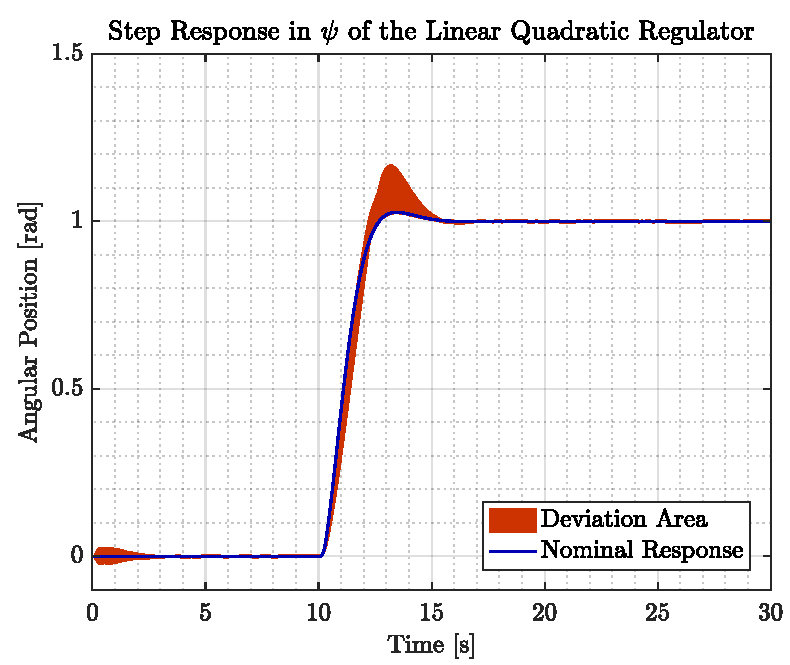
\includegraphics[width=.45\textwidth]{figures/yaw_mc_lqr}         
    }                                                                    
    \hspace{5pt}                                                          
    \captionbox  
    {   
        Step response in $\psi$ of the $\mathcal{H}_\infty$ Controller, where the nominal response, the maximum variation region and the 1-$\sigma$ region are shown.   
        \label{fig:yaw_mc_rob}
    }                                                                          
    {
        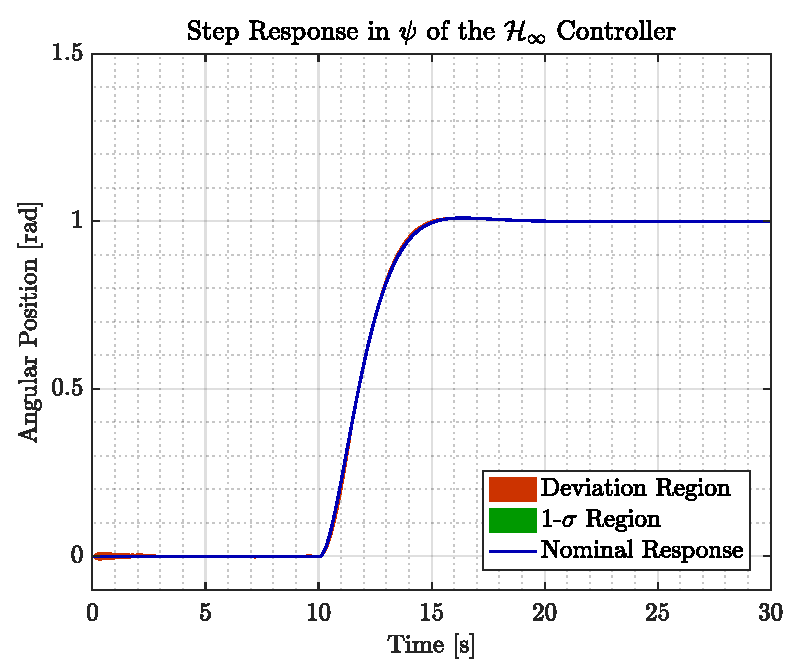
\includegraphics[width=.45\textwidth]{figures/yaw_mc_rob}
    }
\end{figure}

The behavior seen in these figures resembles that for \autoref{fig:xbdot_mc_lqr} and \ref{fig:xbdot_mc_rob}. The $\mathcal{H}_\infty$ Controller shows less overshoot and variability in the different simulations but it is also slightly slower that the LQR controller. In both cases, the 1-$\sigma$ value is very closed to zero, but the reponse of the Linear Quadratic Regulator shows a maximum variation of 20\%.
%In order to achieve a proper comparison, the variance with respect to the nominal model response in abscense of disturbances has been calculated. For the LQR controller, the variance is \fxnote{Write variance for LQR}, while that for the $\mathcal{H}_\infty$ Controller is \fxnote{write variance for robust}.

As in the case of $\dot{x}_\mathrm{b}$, a close look at the difference with respect tot the nominal response can be seen in \autoref{fig:yaw_mc_lqr_error} and \ref{fig:yaw_mc_rob_error}.
\begin{figure}[H]
    \captionbox 
    {   
        Difference with the nominal behavior in $\psi$ of the Linear Quadratic Regulator, where the maximum variation region and the 1-$\sigma$ region are shown.
        \label{fig:yaw_mc_lqr_error}
    }                                                                 
    {                                                                  
        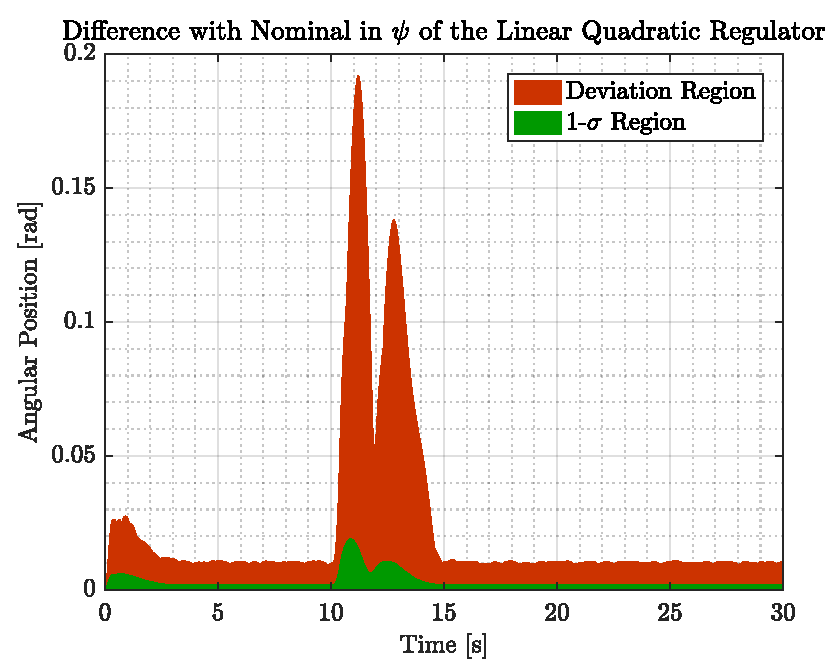
\includegraphics[width=.45\textwidth]{figures/yaw_mc_lqr_error}         
    }                                                                    
    \hspace{5pt}                                                          
    \captionbox  
    {   
        Difference with the nominal behavior in $\psi$ of the $\mathcal{H}_\infty$ Controller, where the maximum variation region and the 1-$\sigma$ region are shown.   
        \label{fig:yaw_mc_rob_error}
    }                                                                          
    {
        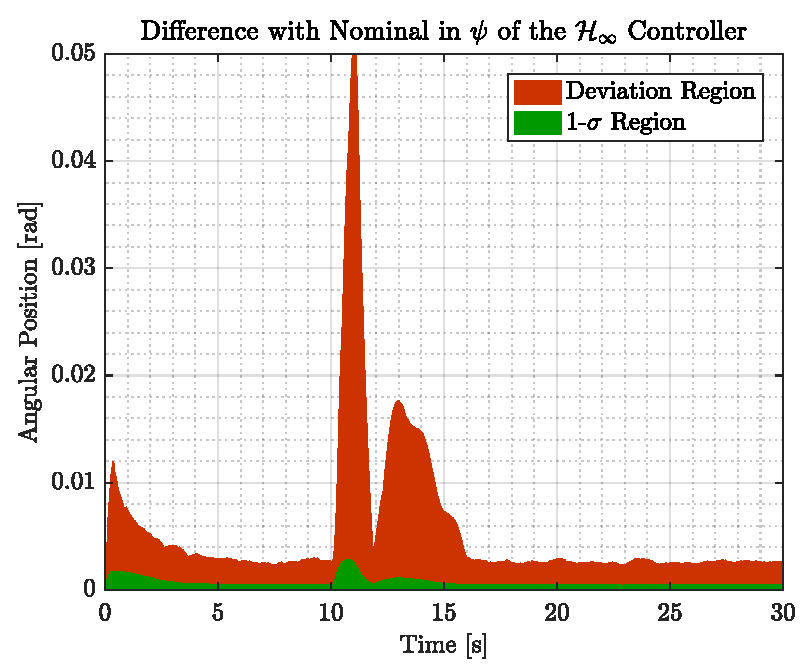
\includegraphics[width=.45\textwidth]{figures/yaw_mc_rob_error}
    }
\end{figure}

In this case, it is also the $\mathcal{H}_\infty$ Controller the one that is able to handle better the disturbances and with less variations with respect to the nominal behavior.

These controller designs are also compared by their usage of inputs. The mean force applied at each time by the thrusters when simulating the LQR controller is \num{17.5793} N, while that of the $\mathcal{H}_\infty$ Controller is \num{17.9281} N. This results as expected since the Linear Quadratic Regulator is designed to optimize the use of inputs to the system.

Finally, to combine performance and usage of inputs, the cost used in the LQR design is calculated as 
%
\begin{flalign}
    J = \sum_{k=0}^\infty \vec{x}_k^\mathrm{T}\vec{Q}\vec{x}_k + \vec{u}_k^\mathrm{T}\vec{R}\vec{u}_k \ .
\end{flalign}

The mean cost among the simulations is \num{7.1441}$\cdot 10^5$ and \num{3.4227}$\cdot 10^6$ for the LRQ and $\mathcal{H}_\infty$ Controller designs. As expected, the cost is lower for the LQR design as minimizing it is the basis of the LQR approach.




    
    %---------- Chapter 8 ---------------------------------------- Path Following
    \chapter{Outer Controller Design}\label{chap:outerController}
The vessel's functionality, as stated in \autoref{sec:requirements}, requires it to follow a path along which the bathymetric measurements are taken. \fxnote{This path should be followed as precisely as possible in the interest area. Depending on functional requirements}. The approach taken to survey an area of interest is to divide the area into straight line segments. The path is generated by dividing the straight line segments into a number of waypoints.

The generated path is followed by using an enclosure based steering algorithm \cite[pp. 258-265]{TFossen} that uses the waypoints along the path. This algorithm follows the waypoints using straight lines only. The outputs of the outer controller are the reference for the yaw angle and the velocity along the $x_\mathrm{b}$ axis, which are inputs to the state space controller designed in \autoref{chap:control}. \fxnote{Provisional header}
    \section{Path Generation Algorithm}\label{sec:pathgeneration}

\fxnote{Check if all variables are correct}The path generation algorithm creates a list of waypoints for the vessel to follow. The area that needs to be surveyed is used to generate the waypoints. The desired area is a bounded rectangle and is given as an input to the algorithm as four coordinates, in \autoref{eq:pathgenxy}, that specifies the start and end coordinates of the area.
%
\begin{flalign} 
  \{x_1; y_1\},       \rule{15px}{0px} 
  \{x_2; y_2\},       \rule{15px}{0px}
  \{x_3; y_3\},       \rule{15px}{0px} 
  \{x_4; y_4\}.       \rule{15px}{0px} 
  \label{eq:pathgenxy}
\end{flalign}
%
\begin{where}
  \va{\{x_k; y_k\}}{is the coordinate of the corner of the bounded rectangle}{}
\end{where}

The path generation algorithm is confined to generate waypoints in an area that is a rectangle. Thus, the four input coordinates need to be verified to ensure the area is a rectangle. This is done by checking
\begin{flalign} 
  \sqrt{(x_1 - x_2)^2 + (y_1 - y_2)^2} &= \sqrt{(x_3 - x_4)^2 + (y_3 - y_4)^2} \\
  \sqrt{(x_1 - x_4)^2 + (y_1 - y_4)^2} &= \sqrt{(x_2 - x_3)^2 + (y_2 - y_3)^2} \\
%   \label{eq:pathgenlengths}
% \end{flalign}
% \begin{flalign}
  \sin{\frac{y_1 - y_2}{x_1 - x_2}} - \sin{\frac{y_1 - y_4}{x_1 - x_4}}  &= \frac{\pi}{2} 
  \label{eq:pathgen}
\end{flalign}
%
Now that the desired area is well defined, as a rectangle, the path generation algorithm is able to generate a list of waypoints for the USV to follow in the given area. \\The path is generated with straight lines and turns for which the vessel shall follow. This pattern is chosen as bathymetric measurements are typically performed in straight lines \fxnote{source}.To determine the width between these lines, the dynamics of the vessel, the swath angle of the multibeam echosounder and the minimum depth of the area to survey were taken into consideration. The swath angle and minimum depth of the Port of Aalborg survey in \autoref{app:bathymetricMapPortOfAalborg} were used to calculate the width between straight lines, as described in \autoref{sec:designconsiderations},
%
\begin{flalign}
  w_\mathrm{beam} = 36 \mathrm{m}
\end{flalign}
\begin{where}
  \va{w_\mathrm{beam}}{is the minimum required beamwidth}{}
\end{where}

The dynamics of the vessel also needs to be considered to ensure the vessel can perform smooth turns between straight lines. It is determined that the vessel capable of using the turning radius 
%
\begin{flalign}
  R_\mathrm{turn} = \frac{1}{2} w_\mathrm{beam} = 18 \mathrm{m}
\end{flalign}
\begin{where}
  \va{R_\mathrm{turn}}{is the turning radius of the waypoints}{}
\end{where}

The path generation algorithm first determines whether to generate waypoints along the x axis or the y axis. This is done to ensure the vessel will perform the least number of turns and is determined by calculating whether the x or y distance is greater. This is done by checking if
%
\begin{flalign}
	(x_\mathrm{end}-x_\mathrm{start}) \geq (y_\mathrm{end}-y_\mathrm{start})
\end{flalign}
%
Once the sailing direction is chosen, the first waypoint is generated using the starting point's coordinates and the direction of the straight lines. The starting point in the transversal direction is offset by $R_\mathrm{turn}$ so the multibeam is able to survey the from the edges of the area.

The number of waypoints on both the straight lines and on the turns are generated using
%
\begin{flalign}
  d_\mathrm{wps} = 50 \mathrm{m} \\
  n_\mathrm{wps} = 10
\end{flalign}
\begin{where}
  \va{d_\mathrm{wps}}{is the distance between waypoints on the straight line}{}
  \va{n_\mathrm{wps}}{is the number of waypoints on each turn}{}
\end{where}

As the area to survey may vary, the waypoints are generated every $d_\mathrm{wps}$ meters to ensure the boat will follow the designated path using these waypoints. Thus, the boat will not rely only on the waypoints that define the area. The path for turns is fixed $R_\mathrm{turn}$ therefore the number of waypoints are fixed to $n_\mathrm{wps}$.

In \autoref{fig:pathgen1} an example of the desired area to survey and the generated waypoints is shown. It can be seen that the vessel is offset by $R_\mathrm{turn}$ and the minimum area the  multibeam sensor surveys is also shown.
%
\begin{figure}[H]
  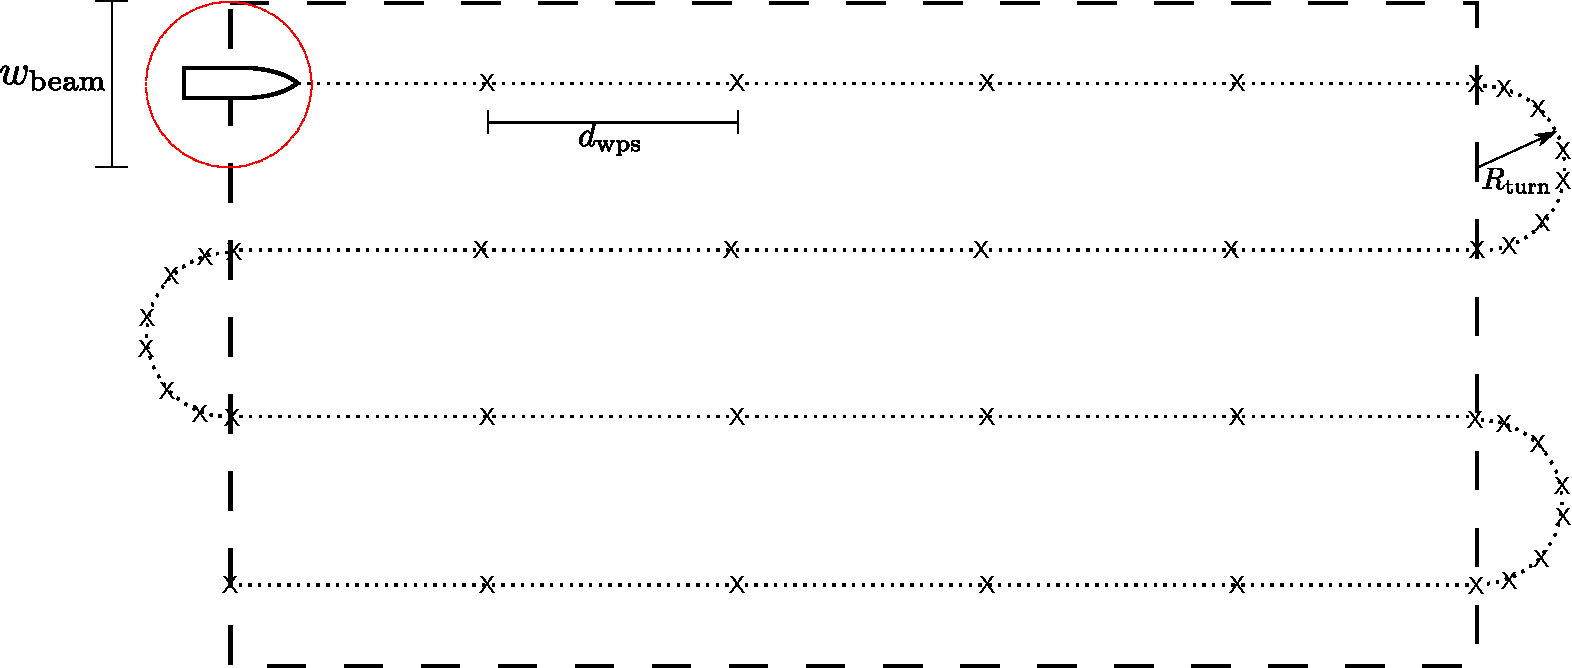
\includegraphics[width=1\textwidth]{figures/pathGen} 
  \caption{Area wanted to survey with waypoints}
  \label{fig:pathgen1}
\end{figure}   



    \section{Path Following Algorithm}
The path generated is approximated by straight line segments connected by waypoints. The vessel then follows these in order to track the path and cover the area in which the measurements are to be taken. This approximation is suitable as the bathymetric measurements are usually taken in straight line paths. If curved paths were required, the solution would be to sample the path with higher frequency in curved sections. \autoref{fig:pathandwaypoints} shows an example of how a path is approximated by straight line segments and waypoints.
\begin{figure}[H]
	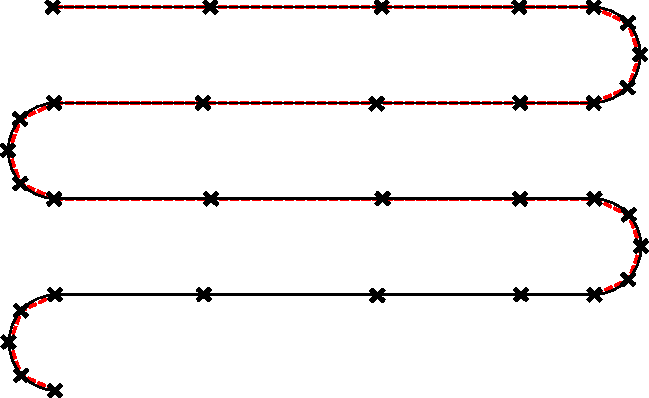
\includegraphics[width=0.6\textwidth]{figures/pathandwpts}
	\caption{A predefined path and its approximation as straight line segments using waypoints.}
	\label{fig:pathandwaypoints}
\end{figure}
The algorithm starts by considering the first two waypoints in the path. The yaw reference given to the state space controller is calculated based on the crossing point between the straight line segment that joints the waypoints and a circle centered in the position of the boat. \autoref{fig:LOSalgorithm} shows how this crossing point is obtained. The point is also called LOS (Line Of Sight) point and is found using the equations of the circle and of the straight line as
%
\begin{flalign}
	(&x_\mathrm{los}-x_\mathrm{n})^2 + (y_\mathrm{los}-y_\mathrm{n})^2 = R^2, \label{eq:circle} \ \\
	&y_\mathrm{los}-y_\mathrm{k} = \frac{y_\mathrm{k+1}-y_\mathrm{k}}{x_\mathrm{k+1}-x_\mathrm{k}}(x_\mathrm{los}-x_\mathrm{k}) \label{eq:line} 
\end{flalign}
\begin{where}
	\va{R}{is the radius of the circle centered at the vessel position}{}
	\va{[x_\mathrm{los},y_\mathrm{los}]}{is the crossing point between the circle around the vessel and the straight line that joins the waypoints}{}
	\va{[x_\mathrm{k},y_\mathrm{k}]}{is the first waypoint in the currently followed path segment}{}
	\va{[x_\mathrm{k+1},y_\mathrm{k+1}]}{is the second waypoint in the currently followed path segment}{}
	\va{[x_\mathrm{n},y_\mathrm{n}]}{is the position of the vessel in the NED frame}{}
\end{where}
%
\begin{figure}[H]
	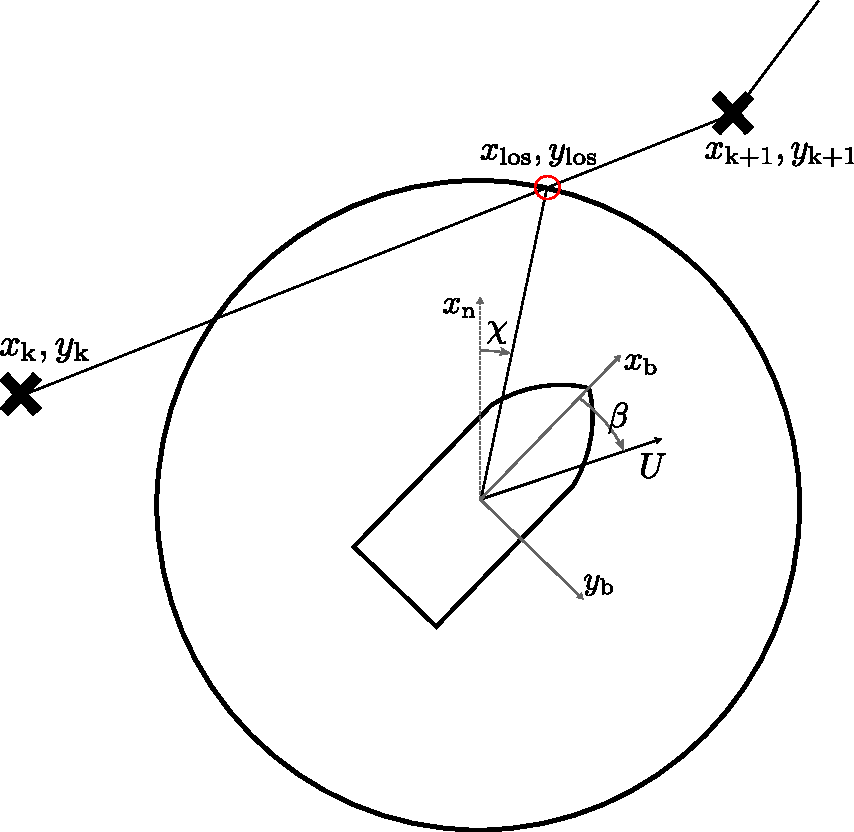
\includegraphics[width=0.5\textwidth]{figures/LOSalgorithm}
	\caption{Algorithm used to find the yaw reference for the state space controller in order to follow a path.}
	\label{fig:LOSalgorithm}
\end{figure}
The LOS point is then used to calculate $\chi$ as the angle from the $x_\mathrm{n}$ axis and the line joining the position of the vessel and the LOS point. See \eqref{eq:chi}. This can be directly used as the reference for yaw, $\psi_\mathrm{ref}$, in the state space controller. This disregards the possibility of disturbances and assumes that the velocity vector of the vessel is aligned with the $x_\mathrm{b}$ axis. This is in general not true as disturbances like wind or waves would generate some speed also in the $y_\mathrm{b}$ axis direction. The reference for yaw is then adjusted by subtracting the angle that the velocity vector has with respect to the $x_\mathrm{b}$ axis as seen in \eqref{eq:beta} and \eqref{eq:psiref}. 

This approach tries to make the vessel velocity vector point towards the LOS point.
%
\begin{flalign}
	\chi &= \arctan\left(\frac{y_\mathrm{los}-y_\mathrm{n}}{x_\mathrm{los}-x_\mathrm{n}}\right), \label{eq:chi} \ \\
	\beta &= \arctan\left(\frac{\dot{y}_\mathrm{b}}{\dot{x}_\mathrm{b}}\right) \label{eq:beta}, \ \\
	\psi&_\mathrm{ref} = \chi - \beta. \label{eq:psiref}
\end{flalign}
\begin{where}
	\va{\chi}{is the angle between the $x_\mathrm{n}$ axis and the LOS point}{}
	\va{\beta}{is the angle between the velocity vector of the vessel and the $x_\mathrm{b}$ axis}{}
\end{where}
%
The algorithm relies on the path and the circle defined around the boat to cross at the LOS point. 

If the vessel is positioned far from the path such that the circle does not intersect it, then the algorithm uses the next waypoint as LOS point. Once the vessel gets closer to the path, the LOS point is calculated as described above.

In order to follow all the path, a way to change which two waypoints define the current path segment needs to be established. Several possibilities can be considered but all of them change active waypoints when the vessel gets close enough to the waypoint that defines the end of the segment. In the project at hand, the distance to the waypoint is evaluated as the distance from the waypoint to the intersection point of the path segment and a perpendicular line to the segment that passes through the vessel position. This distance is depicted in \autoref{fig:changewaypoints}.
\begin{figure}[H]
	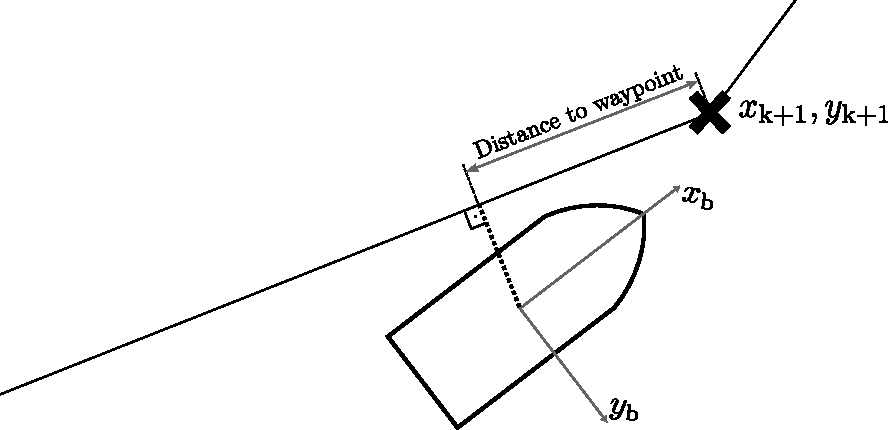
\includegraphics[width=0.6\textwidth]{figures/LOSalgorithmdistancewp}
	\caption{The distance considered when defining the criterion to change to new waypoints.}
	\label{fig:changewaypoints}
\end{figure}
With this approach, the vessel will always try to move forward in the path although a waypoint position has not been precisely attained. % This avoids situations like the one shown in \autoref{fig:goingbackapproach} where the vessel turns around in order to hit the waypoint precisely.
This could be caused by a sudden disturbance experienced by the vessel and, in general, it is desired to keep following the path rather than turning around to hit the waypoint. In most cases, the vessel itself is going to be close to the waypoint when the change occurs. This can be seen in the simulation plots presented below. 

\subsection{Path Following Algorithm Simulation}

\fxnote{Do not include many graphs now because we will probably redo them. Just some dummy ones.} 
\fxnote{Maybe we could include the result also with different low level controllers}
The path following algorithm has been tested in the same path and considering different settings for the algorithm. In all cases, the radius of the circle defined around the vessel is 5 m and the distance in which the active waypoints are changed is 3 m. 

In \autoref{fig:simpleLOSalgorithm} and \ref{fig:simpleLOSalgorithmdisturbance} the results of the algorithm are presented when considering the simpler case in which $\psi_\mathrm{ref} = \chi$, that is, assuming the velocity of the vessel is pointing along the $x_\mathrm{b}$ direction. In the first graph the path is followed precisely as the assumption regarding the velocity vector holds,  whereas in the second, the constant disturbance imposes an offset in the position of the vessel.
\begin{figure}[H]
	\captionbox  %<--use captionbox instead if no global caption is needed
	{               %                                \%-%-%-%-%-%-%\
	 	Performance of the path following algorithm based on $\psi_\mathrm{ref}=\chi$.                %\
		\label{fig:simpleLOSalgorithm}                                  %\
	}                                                                 %\
	{                                                                  %\
		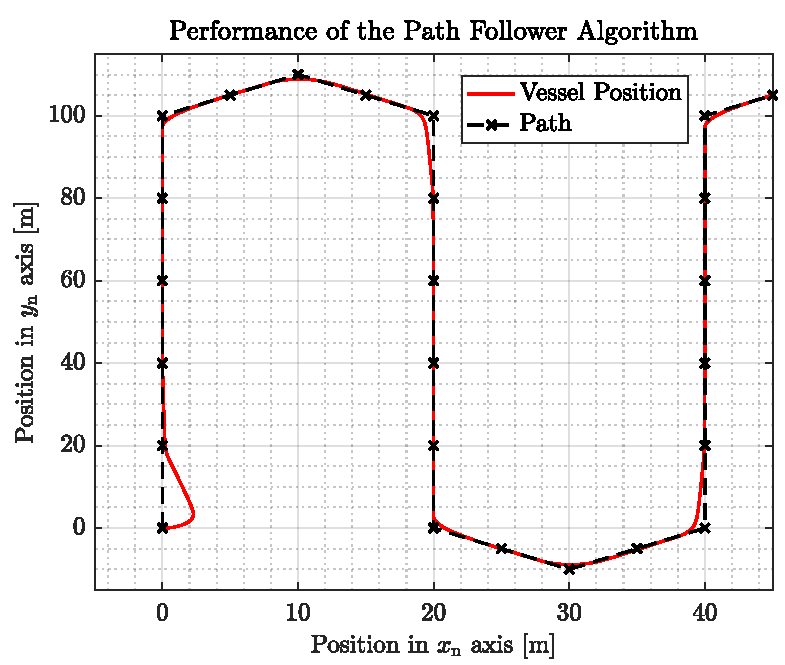
\includegraphics[width=.45\textwidth]{figures/pathfollowingsimple}         %\
	}                                                                    %\
	\hspace{5pt}                                                          %\
	\captionbox  %<-----------------------------------------------------%\
	{       
		Performance of the path following algorithm based on $\psi_\mathrm{ref}=\chi$. The vessel is experiencing a constant disturbance force of 1 N applied with an angle of $\pi/2$.                                                                  %\                         %\
		\label{fig:simpleLOSalgorithmdisturbance}                                     %\
	}                                                                           %\
	{                                                                            %\
		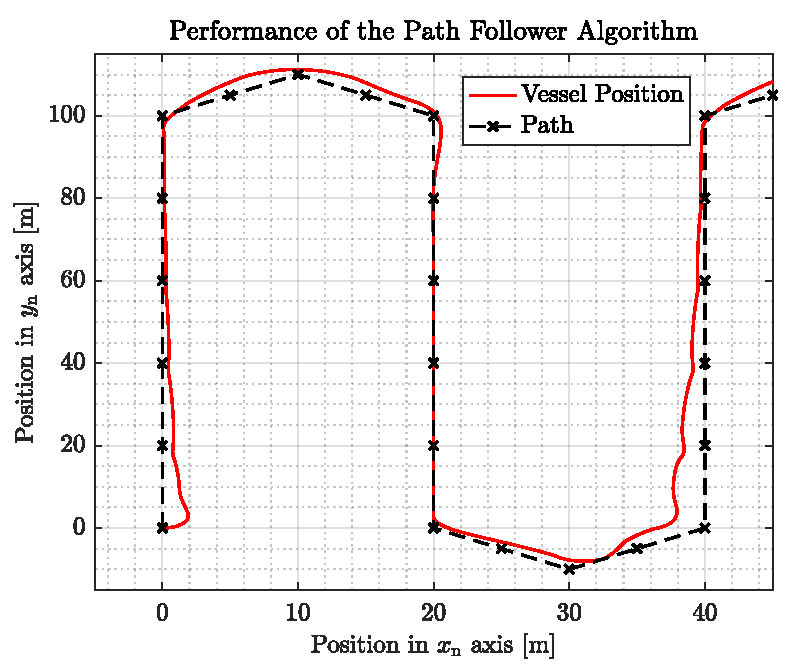
\includegraphics[width=.45\textwidth]{figures/pathfollowingsimpledist}            %|
	}                                                                             %|
\end{figure}
When the information of the vessel velocity is used to calculate the reference angle, $\psi_\mathrm{ref}$, the disturbance is rejected. This is seen in \autoref{fig:normalLOSalgorithmdisturbance}, where the vessel is experiencing the same disturbance as in \autoref{fig:simpleLOSalgorithmdisturbance}. In this case, the offset in position has been corrected and the path is precisely followed.
\begin{figure}[H]
	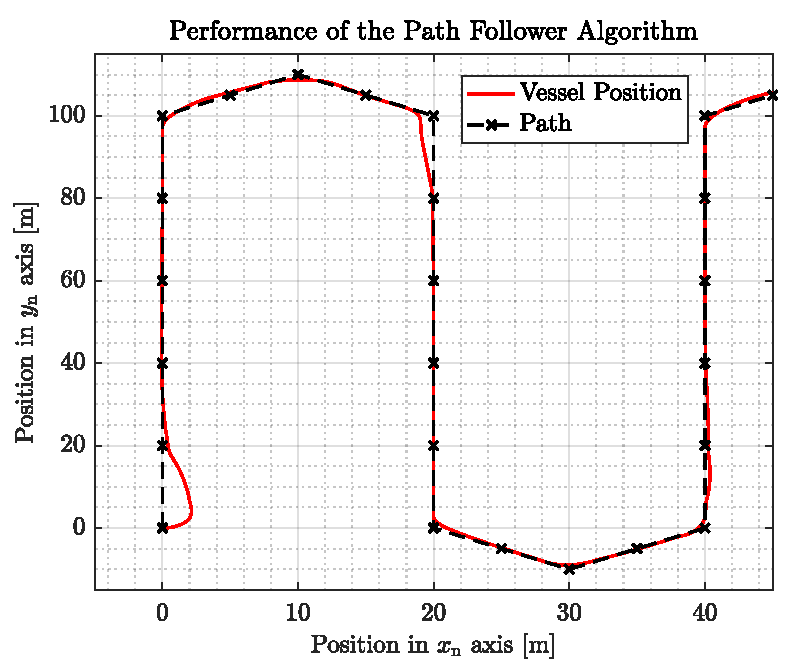
\includegraphics[width=0.6\textwidth]{figures/pathfollowingcomplex}
	\caption{Performance of the path following algorithm based on $\psi_\mathrm{ref}=\chi-\beta$. The vessel is experiencing a constant disturbance force of 1 N applied with an angle of $\pi/2$.}
	\label{fig:normalLOSalgorithmdisturbance}
\end{figure}
According to the results of the simulations, it can be said that the vessel hits the waypoints precisely when they are part of a straight line section of the path. In curved sections, the vessel joins smoothly the straight line segments that approximate the curve. In many cases, and especially for bathymetric measurements the algorithm can be considered suitable.

	




    \section{Simulation Results}
The path following algorithm has been tested in the same path and considering different settings for the algorithm. In all cases, the distance in which the active waypoints are changed is \num{1} m. For seeing the results, the nonlinear model of the system has been simulated with the path following algorithm and the two inner controller designs. In the plots presented, the data from 100 simulations is depicted, where the disturbances, model uncertainties and noise affect the system.

The wind disturbance varies randomly from $\pm$\num{1.5} N in force along $x_\mathrm{b}$ and $y_\mathrm{b}$ and from $\pm$\num{1.5} Nm in torque in $\psi$. The waves are assumed to be sinusoidal with amplitude of 1N and a frequency that goes from 0 to 10 Hz. This disturbance is applied along $x_\mathrm{b}$ and $y_\mathrm{b}$. 

The uncertainty considered is of 20\% in all parameters of the model, that is, the added masses, $m_\mathrm{x}$ and $m_\mathrm{y}$, the moment of inertia around the $z_\mathrm{b}$ axis, $I_\mathrm{z}$, the damping coefficients, $d_\mathrm{x}$, $d_\mathrm{y}$ and $d_\psi$, and the vessel lengths, $l_1$ and $l_2$.  

In \autoref{fig:lqrwrong}, \ref{fig:distlqrwrong}, \ref{fig:robwrong} and \ref{fig:distrobwrong} the results of the algorithm are presented by depicting the path taken by the vessel and the distance to the target path. In these figures, the path following algorithm corresponds to the simpler case in which $\psi_\mathrm{ref} = \chi$, that is, assuming the velocity of the vessel is pointing along the $x_\mathrm{b}$ direction. The simulations are performed with both inner controller designs. 

\begin{figure}[H]
	\captionbox  %<--use captionbox instead if no global caption is needed
	{  
		Performance of the path following algorithm based on $\psi_\mathrm{ref}=\chi$ and using the LQR inner controller. The system is experiencing wind and wave disturbances, model perturbations and measurement noise.\label{fig:lqrwrong}                                
	}                                                                 
	{                                                                  
		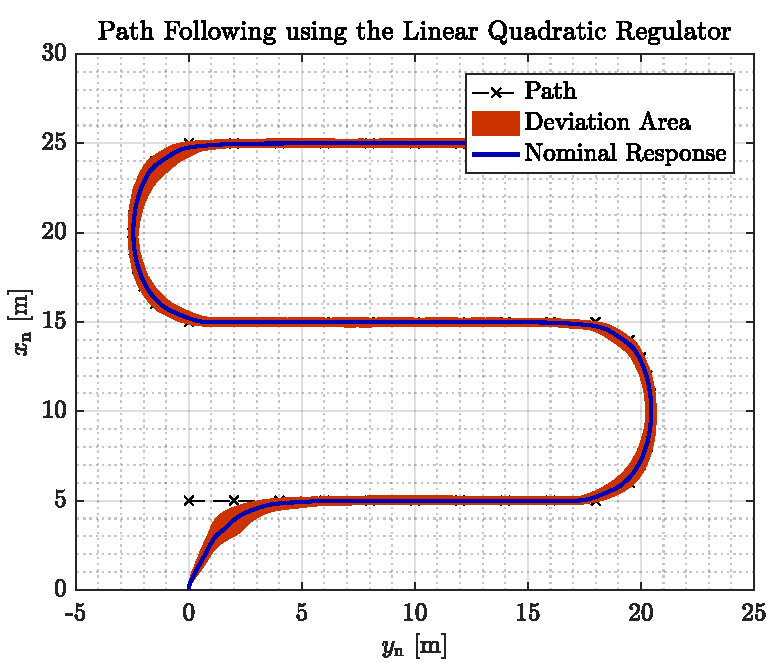
\includegraphics[width=.45\textwidth]{figures/path_lqr_no_correc}         
	}                                                                    
	\hspace{5pt}                                                  
	\captionbox
	{       
		Distance to the path when using the algorithm based on $\psi_\mathrm{ref}=\chi$ and the LQR inner controller .The system is experiencing wind and wave disturbances, model perturbations and measurement noise.
		\label{fig:distlqrwrong}                               
	}                                                                  
	{                                                                    
		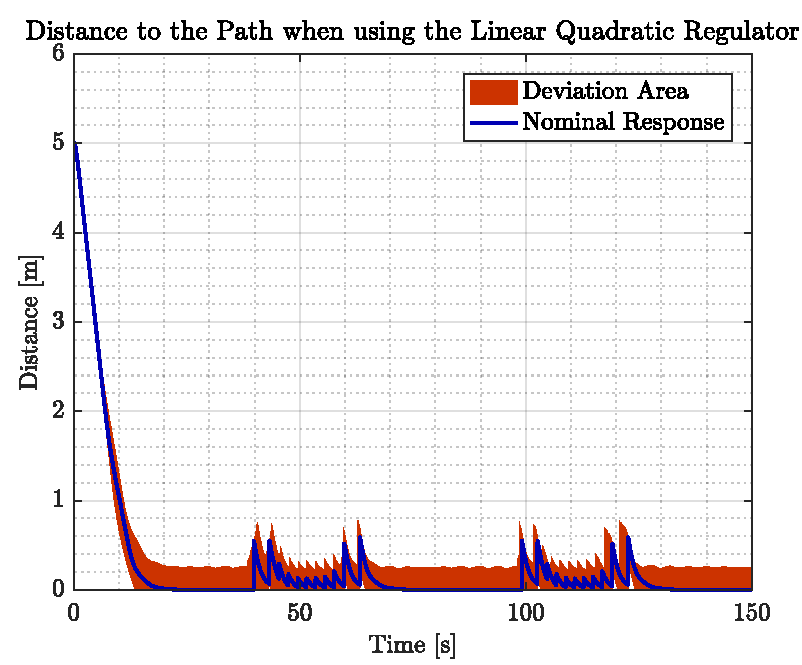
\includegraphics[width=.45\textwidth]{figures/dist_lqr_no_correc}         
	}                                                                         
\end{figure}
\begin{figure}[H]
	\captionbox 
	{   
		Performance of the path following algorithm based on $\psi_\mathrm{ref}=\chi$ and using the $\mathcal{H}_\infty$ inner controller. The system is experiencing wind and wave disturbances, model perturbations and measurement noise.\label{fig:robwrong}
	}                                                                 
	{                                                                  
		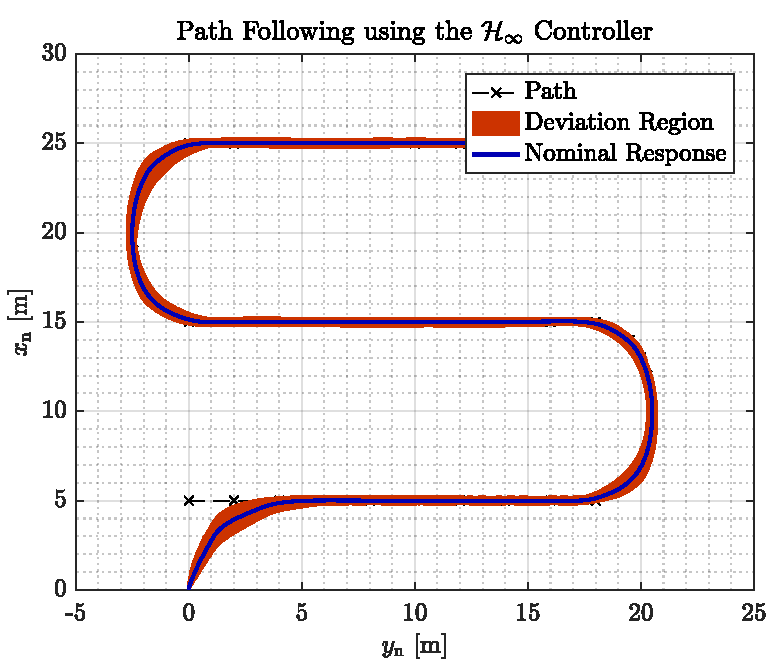
\includegraphics[width=.45\textwidth]{figures/path_rob_no_correc}         
	}                                                                    
	\hspace{5pt}                                                          
	\captionbox  
	{      
		Distance to the path when using the algorithm based on $\psi_\mathrm{ref}=\chi$ and the $\mathcal{H}_\infty$ inner controller .The system is experiencing wind and wave disturbances, model perturbations and measurement noise.\label{fig:distrobwrong}
	}                                                                          
	{
		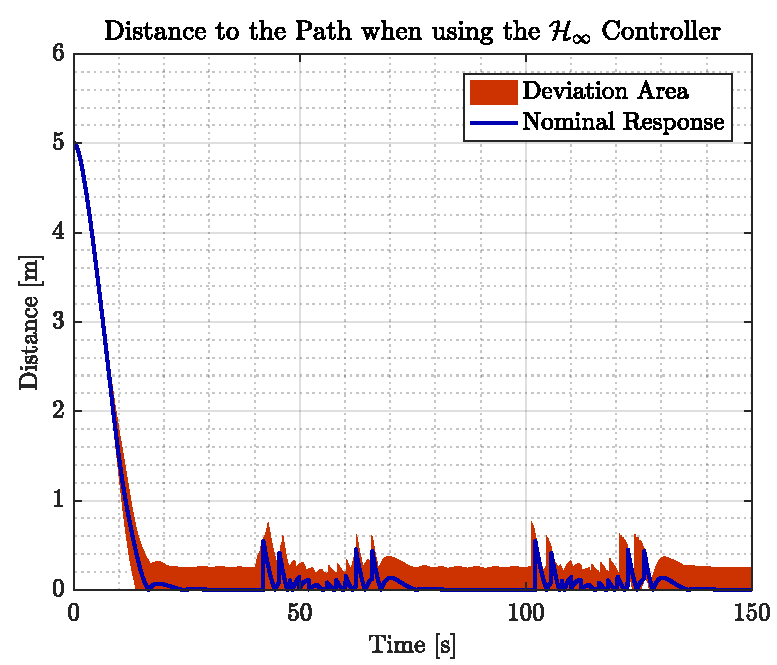
\includegraphics[width=.45\textwidth]{figures/dist_rob_no_correc}
	}
\end{figure}

In these graphs, it is clear that the path is not precisely followed when disturbances are introduced in the system. This offset is expected as the assumption for this simpler algorithm to work does not hold with disturbances like wind and waves. The latter is specially visible in the straight line parts of the path, where the vessel movement shows a 1-$\sigma$ value that goes up to 10 cm and a maximum value that reaches up to approximately 30 cm.

When the information of the vessel velocity is used to calculate the reference angle, $\psi_\mathrm{ref}$, the disturbance is rejected. This is seen in \autoref{fig:lrqcorrect}, \ref{fig:distlqr}, \ref{fig:robustcorrect} and \ref{fig:distrobustcorrect}, where the vessel is experiencing disturbances and model perturbations in the same range as in the previously shown figures. Both the vessel X-Y movement and the distance to the target path are depicted. 

\begin{figure}[H]
	\captionbox  %<--use captionbox instead if no global caption is needed
	{               %                                \%-%-%-%-%-%-%\
		Performance of the path following algorithm based on $\psi_\mathrm{ref}=\chi-\beta$ and using the LQR inner controller. The system is experiencing wind and wave disturbances, model perturbations and measurement noise.                %\
		\label{fig:lrqcorrect}                                  %\
	}                                                                 %\
	{                                                                  %\
		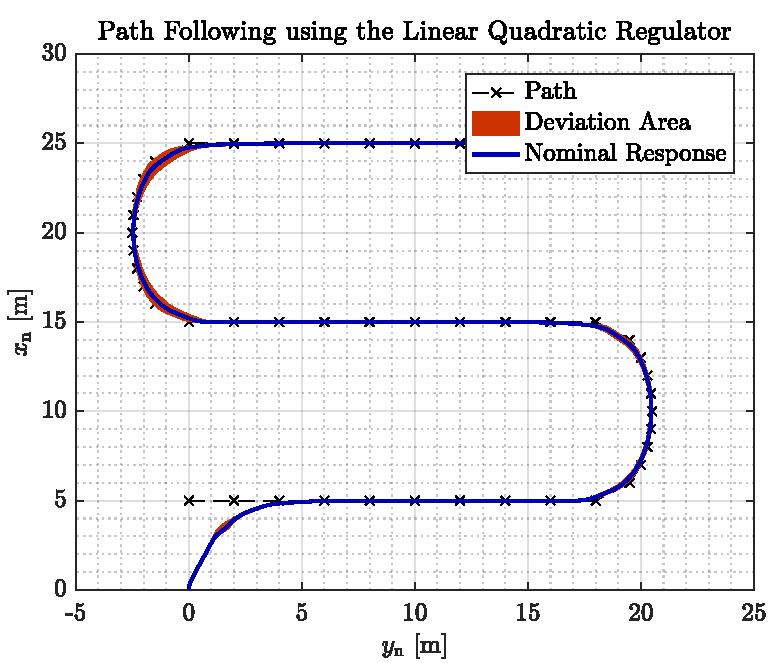
\includegraphics[width=.45\textwidth]{figures/path_lqr}         %\
	}                                                                    %\
	\hspace{5pt}                                                          %\
	\captionbox  %<-----------------------------------------------------%\
	{       
			Distance to the path when using the algorithm based on $\psi_\mathrm{ref}=\chi-\beta$ and the LQR inner controller .The system is experiencing wind and wave disturbances, model perturbations and measurement noise.                                                                  %\                         %\
		\label{fig:distlqr}                                     %\
	}                                                                           %\
	{                                                                            %\
		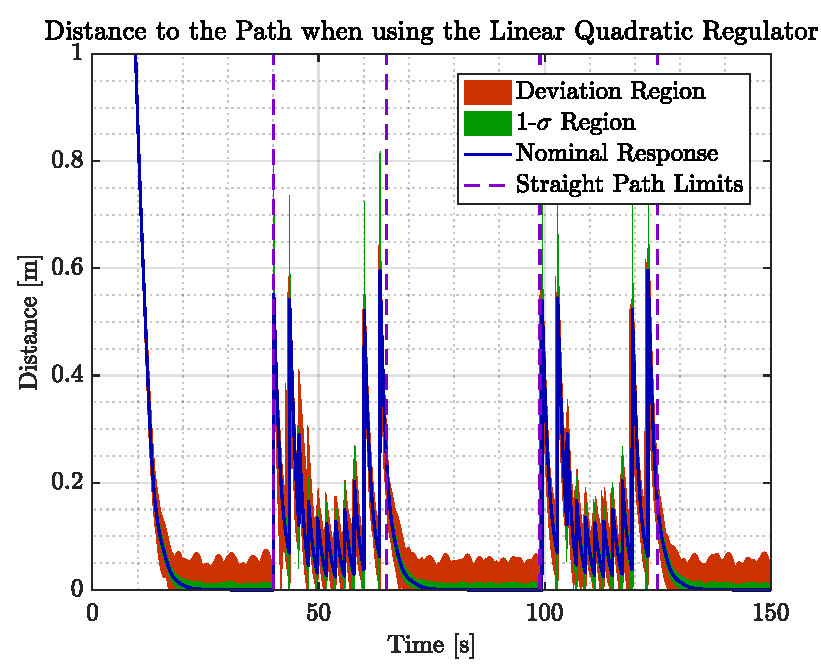
\includegraphics[width=.45\textwidth]{figures/dist_lqr}            %|
	}                                                                             %|
\end{figure}
\begin{figure}[H]
	\captionbox 
	{   
		Performance of the path following algorithm based on $\psi_\mathrm{ref}=\chi-\beta$ and using the $\mathcal{H}_\infty$ inner controller. The system is experiencing wind and wave disturbances, model perturbations and measurement noise. \label{fig:robustcorrect}
	}                                                                 
	{                                                                  
		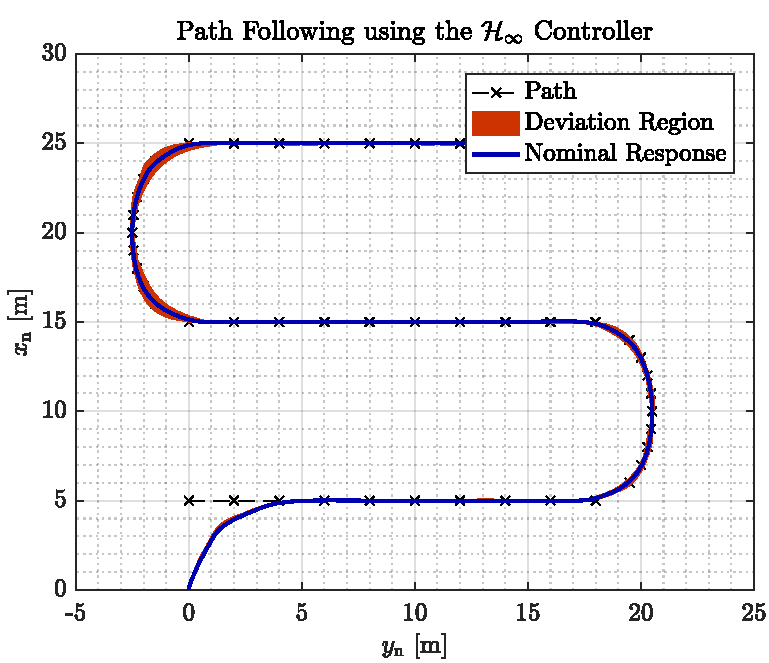
\includegraphics[width=.45\textwidth]{figures/path_rob}         
	}                                                                    
	\hspace{5pt}                                                          
	\captionbox  
	{      
			Distance to the path when using the algorithm based on $\psi_\mathrm{ref}=\chi-\beta$ and the $\mathcal{H}_\infty$ inner controller .The system is experiencing wind and wave disturbances, model perturbations and measurement noise.\label{fig:distrobustcorrect}
	}                                                                          
	{
		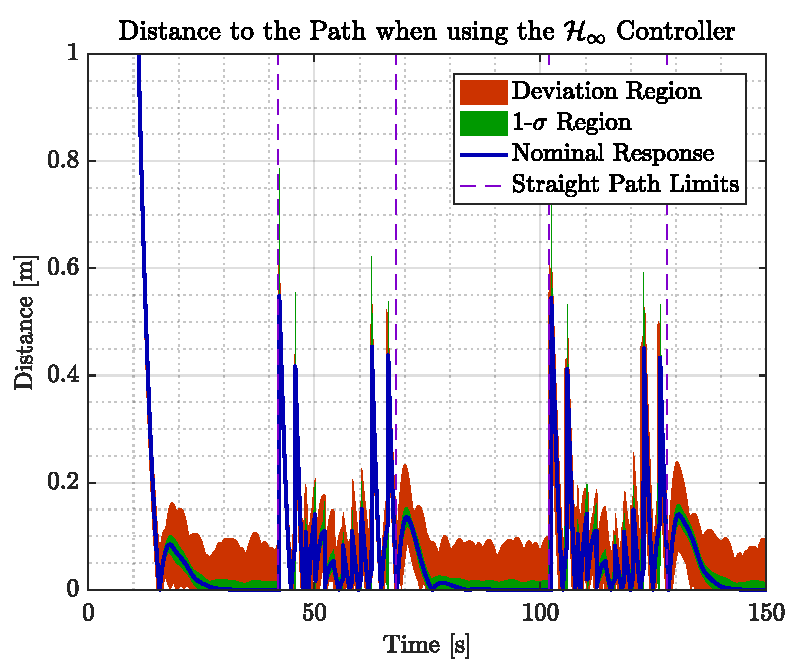
\includegraphics[width=.45\textwidth]{figures/dist_rob}
	}
\end{figure}

In this case, the offset in position has been corrected and the path is followed within the desired precision in the straight line segments. There are still some small deviations due to the wave disturbance present in the system, but the 1-$\sigma$ value is almost below 5 cm and the maximum variations stay below 10 cm with respect to the reference path.

According to the results of the simulations, it can be said that the vessel follows the path through the waypoints when they are part of a straight line section of the path. In curved sections, the vessel joins smoothly the straight line segments that approximate the curve. In many cases, and especially for bathymetric measurements, the algorithm can be considered suitable.
    
    %---------- Chapter 9 ---------------------------------------- Sensor Fusion
    \chapter{Sensor Fusion}\label{chap:sensorFusion}



    \section{Attitude Estimation}\label{sec:attFusion}
The attitude estimation is done using a Kalman filter. The estimate contains attitude, angular velocity and angular acceleration information. For constructing the Kalman filter, a process model and a measurement model need to be created. 

The process model describes the dynamics of the system and how the inputs affect its states. The process model includes also noise, which is assumed to be normally distributed. The process model is represented as in \autoref{eq:processmodelatt}. 
The measurement model describes how the measurements taken from the IMU relate with the states of the system represented in the process model. Measurement noise is also included in the model. The process and measurement models are 
%
\begin{flalign}
    \vec{x}_\mathrm{att}(k+1) &= \vec{A}_\mathrm{att}\vec{x}_\mathrm{att}(k) + \vec{B}_\mathrm{att} \vec{u}(k) + \vec{w}_\mathrm{att}(k) \label{eq:processmodelatt} \\
    \vec{y}_\mathrm{att}(k) &= \vec{C}_\mathrm{att} \vec{x}_\mathrm{att}(k) + \vec{v}_\mathrm{att}(k) \label{eq:measurementmodelatt}\ .
\end{flalign}
\begin{where}
	\va{\vec{x}_\mathrm{att}}{is the system state vector for the attitude Kalman filter}{}
	\va{\vec{u}}{is the input vector}{}
	\va{\vec{w}_\mathrm{att}(k)}{is the process noise vector}{}
    \va{\vec{v}_\mathrm{att}(k)}{is the measurement noise vector}{}
    \va{\vec{A}_\mathrm{att}}{is the system matrix for the attitude Kalman filter model}{}
    \va{\vec{B}_\mathrm{att}}{is the input matrix for the attitude Kalman filter model}{}
    \va{\vec{C}_\mathrm{att}}{is the output matrix for the attitude Kalman filter model}{}    
\end{where}
The noise vectors $\vec{w}_\mathrm{att}(k)$ and $\vec{v}_\mathrm{att}(k)$ are independent, and follow a zero mean normal distribution. The covariance matrices of each distribution are $\vec{Q}_\mathrm{att}$ and $\vec{R}_\mathrm{att}$, respectively. These are diagonal matrices calculated as
\begin{flalign}
	\vec{Q}_\mathrm{att} &= \mathrm{diag}\left( \sigma_\mathrm{\phi}^2,\sigma_\mathrm{\theta}^2,\sigma_\mathrm{\psi}^2,\sigma_\mathrm{\dot{\phi}}^2,\sigma_\mathrm{\dot{\theta}}^2,\sigma_\mathrm{\dot{\psi}}^2,\sigma_\mathrm{\ddot{\phi}}^2,\sigma_\mathrm{\ddot{\theta}}^2,\sigma_\mathrm{\ddot{\psi}}^2 \right) \\
	\vec{R}_\mathrm{att} &= \mathrm{diag} \left( \sigma_{\phi\mathrm{,acc}}^2,\sigma_{\theta\mathrm{,acc}}^2,\sigma_{\psi\mathrm{,mag}}^2,\sigma_{\dot{\phi}\mathrm{,gyro}}^2,\sigma_{\dot{\theta}\mathrm{,gyro}}^2,\sigma_{\dot{\psi}\mathrm{,gyro}}^2 \right)
\end{flalign}
\fxnote{say how we calculate these variances, refer to an appendix with values also maybe}
The states chosen for the Kalman model include all variables to be estimated and those in which dynamics of the system play a role. These are
\begin{flalign}
    \vec{x}_\mathrm{att} &= 
    \begin{bmatrix}
       \phi & \theta & \psi & \dot{\phi} & \dot{\theta} & \dot{\psi} & \ddot{\phi} & \ddot{\theta} & \ddot{\psi} \nonumber
    \end{bmatrix}^\mathrm{T} \ .
\end{flalign}
Even though the inner state space controller only considers $\psi$ and $\dot{\psi}$, the other Euler angles and angular velocities are included to allow a better overall estimation, specially when using later the rotation matrix elements as described in \autoref{sec:posFusion}. The angular accelerations are normally not part of a state vector in a state space representation. However, in the attitude Kalman filter state vector, the accelerations are included as they are an important part of the dynamics of the vessel as it can be seen in the last tree rows in $A_\mathrm{att}$, \autoref{eq:Aatt}.

The output vector elements depend on the measurements given by the IMU. These include the angular velocities provided by the gyroscope and the attitude measurements. The latter are obtained from a direct calculation using the accelerometer and magnetometer data \cite{MBibuli} as	
\begin{flalign}
	\phi_\mathrm{acc} &= \arctan\left(\frac{\ddot{y}_\mathrm{b,acc}}{\sqrt{\ddot{x}_\mathrm{b,acc}^2 + \ddot{z}_\mathrm{b,acc}^2}} \right)\ , \label{eq:roll_acc} \\
	\theta_\mathrm{acc} &= \arctan \left( \frac{\ddot{x}_\mathrm{b,acc}}{\sqrt{\ddot{y}_\mathrm{b,acc}^2 + \ddot{z}_\mathrm{b,acc}^2}} \right)\ , \label{eq:pitch_acc} \\
	\psi_\mathrm{mag} &= \arctan \left( \frac{M_{y_\mathrm{b}} \cos(\phi) + M_{z_\mathrm{b}} \sin(\phi)}{M_{x_\mathrm{b}} \cos(\theta) + M_{y_\mathrm{b}} \sin(\phi) \sin(\theta) + M_{z_\mathrm{b}} \cos(\phi) \sin(\theta)} \right)\ .\label{eq:yaw_mag}
\end{flalign}
\begin{where}
	\va{\ddot{x}_\mathrm{b,acc}}{is the measured acceleration along the $x_\mathrm{b}$ direction}{}
	\va{\ddot{y}_\mathrm{b,acc}}{is the measured acceleration along the $y_\mathrm{b}$ direction}{}
	\va{\ddot{z}_\mathrm{b,acc}}{is the measured acceleration along the $z_\mathrm{b}$ direction}{}
	\va{M_{x_\mathrm{b}}}{is the magnetic field strength along the $x_\mathrm{b}$ direction}{}
	\va{M_{y_\mathrm{b}}}{is the magnetic field strength along the $y_\mathrm{b}$ direction}{}
	\va{M_{z_\mathrm{b}}}{is the magnetic field strength along the $z_\mathrm{b}$ direction}{}			
\end{where}

Leading to the output vector 
\begin{flalign}
    \vec{y}_\mathrm{att} =
    \begin{bmatrix}
           \phi_\mathrm{acc} & \theta_\mathrm{acc} & \psi_\mathrm{mag} & \dot{\phi}_\mathrm{gyro} & \dot{\theta}_\mathrm{gyro} & \dot{\psi}_\mathrm{gyro}\nonumber 
    \end{bmatrix}^\mathrm{T}\ .
\end{flalign}

The input vector, in this case stays the same as in the state space controller design, containing the two forces provided by the thrusters. The input vector is
\begin{flalign}
    \vec{u} &=
    \begin{bmatrix}
        F_1 & F_2  \nonumber 
    \end{bmatrix}^\mathrm{T}\ .
\end{flalign}

With this information, the process and measurement model matrices can be built. The $\vec{A}_\mathrm{att}$ matrix is what describes the dynamics of the model. In this system, the attitude is itself plus the discrete integration of the angular velocity over the sampling period. This is represented by the 1 and the T$_s$ in each of the Euler angle rows. The same dynamics describe the angular velocities. The angular accelerations depend on the angular velocities through the damping coefficients. In order to consider the most recent value of the angular velocities, the three last rows of $\vec{A}_\mathrm{att}$ are just a copy of the three middle rows of $\vec{A}_\mathrm{att}$ multiplied by the corresponding damping coefficient and divided by the matching moment of inertia. The elements on these last rows also include the minus sign coming from the damping. The $\vec{A}_\mathrm{att}$ matrix is 
\begin{flalign}
	\label{eq:Aatt}
    \vec{A}_\mathrm{att} &=
    \begin{bmatrix}
    	1 & 0 & 0 & T_\mathrm{s} & 0 & 0 & 0 & 0 & 0 \\
        0 & 1 & 0 & 0 & T_\mathrm{s} & 0 & 0 & 0 & 0 \\
        0 & 0 & 1 & 0 & 0 & T_\mathrm{s} & 0 & 0 & 0 \\
        0 & 0 & 0 & 1 & 0 & 0 & T_\mathrm{s} & 0 & 0 \\
        0 & 0 & 0 & 0 & 1 & 0 & 0 & T_\mathrm{s} & 0 \\
        0 & 0 & 0 & 0 & 0 & 1 & 0 & 0 & T_\mathrm{s} \\
        0 & 0 & 0 & \frac{-d_\mathrm{\phi}}{I_\mathrm{x}} & 0 & 0 & -T_\mathrm{s}\frac{d_\mathrm{\psi}}{I_\mathrm{x}} & 0 & 0 \\
        0 & 0 & 0 & 0 & \frac{-d_\mathrm{\theta}}{I_\mathrm{y}} & 0 & 0 & -T_\mathrm{s}\frac{d_\mathrm{\theta}}{I_\mathrm{y}} & 0 \\
        0 & 0 & 0 & 0 & 0 & \frac{-d_\mathrm{\psi}}{I_\mathrm{z}} & 0 & 0 & -T_\mathrm{s}\frac{d_\mathrm{\psi}}{I_\mathrm{z}}\ . \nonumber
    \end{bmatrix}
\end{flalign}

The matrix $\vec{B}_\mathrm{att}$ is mostly formed by zeros, the only nonzero elements are placed in the last row, indicating how the forces contribute to the angular acceleration in the yaw angle. The $\vec{C}_\mathrm{att}$ matrix is also straightforward to obtain as the measurement are just the first six states in $\vec{x}_\mathrm{att}$. The $\vec{B}_\mathrm{att}$ and $\vec{C}_\mathrm{att}$ matrices are

\begin{minipage}{0.3\linewidth}
    \begin{flalign}
        \vec{B}_\mathrm{att} &=
        \begin{bmatrix}
            0 & 0 \\
            0 & 0 \\
            0 & 0 \\
            0 & 0 \\
            0 & 0 \\
            0 & 0 \\
            0 & 0 \\
            0 & 0 \\
            \frac{l_1}{I_\mathrm{z}} & \frac{-l_2}{I_\mathrm{z}}\nonumber 
        \end{bmatrix} 
    \end{flalign}
\end{minipage}\hfill
\begin{minipage}{0.6\linewidth}
    \begin{flalign}
        \vec{C} &=
        \begin{bmatrix}
            1 & 0 & 0 & 0 & 0 & 0 & 0 & 0 & 0 \\
            0 & 1 & 0 & 0 & 0 & 0 & 0 & 0 & 0 \\
            0 & 0 & 1 & 0 & 0 & 0 & 0 & 0 & 0 \\
            0 & 0 & 0 & 1 & 0 & 0 & 0 & 0 & 0 \\
            0 & 0 & 0 & 0 & 1 & 0 & 0 & 0 & 0 \\
            0 & 0 & 0 & 0 & 0 & 1 & 0 & 0 & 0 \nonumber 
        \end{bmatrix} 
    \end{flalign}
\end{minipage}\hfill

Once the model is constructed, the Kalman filter equations can be obtained. They are divided in two steps, prediction and update \cite{SHaykin}. To start the process, the estimate and error covariance matrix $\vec{P}_\mathrm{att}$ need to be initialized. The state estimation is initilaized with its mean, which is zero and the error covariance matrix is initialized with the covariance matrix for the states. The initialization is done as
\begin{flalign}
	\vec{x}_\mathrm{att}(0|0) &= \vec{0}_\mathrm{1x6}\\
	\vec{P}_\mathrm{att}(0|0) &= \vec{Q}_\mathrm{att}\ .
\end{flalign}
 
\subsection*{Prediction Step}
In the prediction step, the sensor most recent measurement has not been acquired yet and the model of the system is used to predict the state values in the next period. The error covariance is also predicted using the system matrix, $\vec{A}_\mathrm{att}$, and the covariance matrix, $\vec{Q}_\mathrm{att}$, of the process noise vector included in the model.
The prediction step of the Kalman filter is  
\begin{flalign}
	\hat{\vec{x}}_\mathrm{att}(k+1|k) &= \vec{A}_\mathrm{att} \hat{\vec{x}}_\mathrm{att}(k|k) + \vec{B}_\mathrm{att} \vec{u}(k) \label{eq:predictxatt} \\
	\vec{P}_\mathrm{att}(k+1|k) &= \vec{A}_\mathrm{att} \vec{P}_\mathrm{att}(k|k) \vec{A}_\mathrm{att}^\mathrm{T} + \vec{Q}_\mathrm{att} \label{eq:predictPatt}
\end{flalign}

\subsection*{Update Step}
The update step corrects the estimate using the prediction obtained in the previous step and the innovation \cite[p. 7]{SHaykin}, that is, the error between the new measurement and the predicted new measurement. This error updates $\vec{x}_\mathrm{att}$ weighted by the Kalman gain $\vec{K}(k)$. The update step is
The update step of the Kalman filter calculates the updated state estimation and the updated error covariance as 
\begin{flalign}
    \hat{\vec{x}}_\mathrm{att}(k+1|k+1) &= \hat{\vec{x}}_\mathrm{att}(k+1|k) + \vec{K}(k+1) \left[ \vec{y}(k+1) - \vec{C}_\mathrm{att}  \hat{\vec{x}}_\mathrm{att}(k+1|k) \right]\ , \label{eq:updatexatt}\\
    \vec{P}_\mathrm{att}(k+1|k+1) &= \left[ \vec{I} - \vec{K}(k+1) \vec{C}_\mathrm{att}^\mathrm{T} \right] \vec{P}_\mathrm{att}(k+1|k)\ . \label{eq:updatePatt}
\end{flalign}

Being the Kalman gain 
\begin{flalign}
	\vec{K}(k+1) &= \vec{P}_\mathrm{att}(k+1|k) \vec{C}_\mathrm{att}^\mathrm{T} \left[\vec{C}_\mathrm{att} \vec{P}(k+1|k) \vec{C}_\mathrm{att}^\mathrm{T} + \vec{R}_\mathrm{att} \right]^{-1}\ , \label{eq:kalmangainatt}
\end{flalign}
which weights how much the measurements and the prediction affect the estimate of the states. It is calculated using the prediction error covariance matrix, $\vec{P}_\mathrm{att}$, the output matrix, $\vec{C}_\mathrm{att}$, and the covariance matrix for the noise vector included in the measurement model. A more detailed derivation of this gain can be found in \cite[pp. 5-8]{SHaykin}.
\fxnote{Include simulations}

    \subsection{Simulation of the Filter}
The performance of the Kalman filter is tested through simulations. These are performed by applying some arbitrary inputs to the model of the system derived in \autoref{chap:model}. The signals obtained are transformed into measurements by adding noise whose variance is that present in the physical sensors and shown in \autoref{app:IMUVariances}.

The simulations are also used to tune the filters so a good estimation of the states is obtained. The tuning parameters are the elements in the covariance matrix for the states, $\vec{Q}_\mathrm{att}$. The final values obtained are
\begin{flalign}
	\vec{Q}_\mathrm{att} &= \mathrm{diag}\left(0,0,0,0,0,0,0,0,0 \right)
\end{flalign}

It is noticeable that the size of the variances is small and that correlates with the slow dynamics that the vessel shows.\fxnote{maybe don't say this}

The procedure starts by focusing on the estimation of the angular velocities and angular accelerations as these states are mostly dependent on the measurement given by the gyroscope and act as input for the attitude state estimation.

The result with the final state variances is shown in \autoref{fig:sim_yawdot} and \ref{fig:sim_yawddot}, where the estimation for $\dot{\psi}$ and $\ddot{\psi}$ are shown. As it can be seen, both signals are correctly estimated. It is specially remarkable in $\ddot{\psi}$, as there are no direct measurements for this state.
\begin{figure}[H]
	\captionbox 
	{   
		Result of the estimation of the angular velocity around $z_\mathrm{b}$, compared to the real value in the simulation and the measurements.
		\label{fig:sim_yawdot}
	}                                                                 
	{                                                                  
		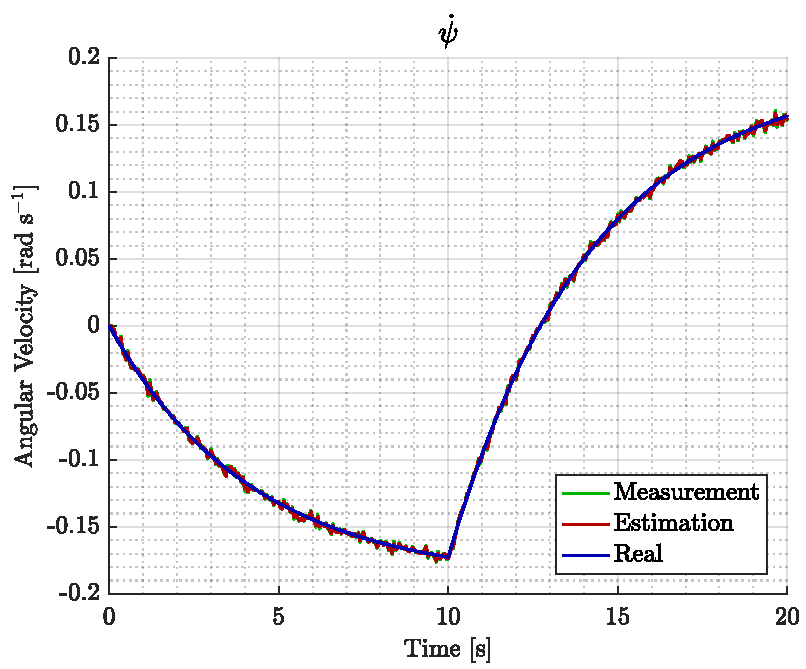
\includegraphics[width=.45\textwidth]{figures/sim_yawdot}         
	}                                                                    
	\hspace{5pt}                                                          
	\captionbox  
	{      
		Estimation of the angular acceleration around $z_\mathrm{b}$, compared to the real value.
		\label{fig:sim_yawddot}
	}                                                                          
	{
		\includegraphics[width=.45\textwidth]{figures/sim_yawddot}
	}
\end{figure}

\autoref{fig:sim_yaw} shows the estimation of the heading, $\psi$ as an example of the attitude estimation of the Kalman filter. This plot is obtained with the final values for the state covariance matrix elements.
\begin{figure}[H]
    \includegraphics[width=0.5\textwidth]{figures/sim_yaw}
    \caption{Result of the estimation of the heading, compared to the real value in the simulation and the measurements.}
    \label{fig:sim_yaw}
\end{figure}
In this case, the filter is also able to remove most of the noise present in the measurement and provide an estimation close to the real value. 
%

%
%\begin{figure}[H]
%    \includegraphics[width=0.5\textwidth]{figures/real_yaw}
%    \caption{}
%    \label{fig:real_yaw}
%\end{figure}
%
%\begin{figure}[H]
%    \captionbox 
%    {   
%        Result of the estimation of the angular velocity around $z_\mathrm{b}$, compared to the measurements.
%        \label{fig:real_yawdot}
%    }                                                                 
%    {                                                                  
%        \includegraphics[width=.45\textwidth]{figures/sim_yawdot}         
%    }                                                                    
%    \hspace{5pt}                                                          
%    \captionbox  
%    {      
%        Estimation of the angular acceleration around $z_\mathrm{b}$.
%        \label{fig:real_yawddot}
%    }                                                                          
%    {
%        \includegraphics[width=.45\textwidth]{figures/real_yawddot}
%    }
%\end{figure}
%
%\cite{MSalari}
    \section{Position Estimation} \label{sec:posFusion}
%The Kalman filter designed for the estimation of the position of the vessel is an Extended Kalman Filter. This variant allows to use the Kalman filter for systems with nonlinear dynamics as it linearizes the system around each estimate by computing the jacobian of the system and the output matrices. \cite[pp. 16-20]{SHaykin}.

As for the attitude Kalman filter, a process model and a measurement model need to be created. These are
\begin{flalign}
    \vec{x}_\mathrm{pos}(k+1) &= \vec{A}_\mathrm{pos}(k)\vec{x}_\mathrm{pos}(k) + \vec{B}_\mathrm{pos} \vec{u}(k) + \vec{w}_\mathrm{pos}(k)\ , \\
    \vec{y}_\mathrm{pos}(k) &= \vec{C}_\mathrm{pos} \vec{x}_\mathrm{pos}(k) + \vec{v}_\mathrm{pos}(k)\ .
\end{flalign}
\begin{where}
    \va{\vec{x}_\mathrm{pos}(k)}{is the system state vector}{}
    \va{\vec{w}_\mathrm{pos}(k)}{is the process noise vector}{}
    \va{\vec{v}_\mathrm{pos}(k)}{is the measurement noise vector}{}
    \va{\vec{A}_\mathrm{pos}(k)}{is the system matrix for the position Kalman filter}{}
    \va{\vec{B}_\mathrm{pos}}{is the input matrix for the position Kalman filter}{}
    \va{\vec{C}_\mathrm{pos}}{is the output matrix for the position Kalman filter}{}    
\end{where}

The noise, $\vec{w}_\mathrm{pos}(k)$ and $\vec{v}_\mathrm{pos}(k)$, are independent zero-mean white Gaussian noise vectors with covariance matrices $\vec{Q}_\mathrm{pos}$ and $\vec{R}_\mathrm{pos}$, respectively. These are 
\begin{flalign}
	\vec{Q}_\mathrm{pos} &= \mathrm{diag} \left( \sigma_\mathrm{x_\mathrm{n}}^2,\sigma_\mathrm{y_\mathrm{n}}^2,\sigma_\mathrm{\dot{x}_\mathrm{b}}^2,\sigma_\mathrm{\dot{y}_\mathrm{b}}^2,\sigma_\mathrm{\ddot{x}_\mathrm{b}}^2,\sigma_\mathrm{\ddot{y}_\mathrm{b}}^2 \right)\\
	\vec{R}_\mathrm{pos} &= \mathrm{diag} \left( \sigma_{x_\mathrm{n}\mathrm{,GPS}}^2,\sigma_{y_\mathrm{n}\mathrm{,GPS}}^2,\sigma_{\ddot{x}_\mathrm{b}\mathrm{,acc}}^2,\sigma_{\ddot{y}_\mathrm{b}\mathrm{,acc}}^2 \right)
\end{flalign}
 
The state vector for this Kalman filter is formed by the position in the NED frame, the velocity in the body frame and the accelerations in the body frame. These variables are either needed in the outer path follower controller or they describe an important part of the dynamics of the system. The position and velocity are on the former group while the accelerations is in the latter. It can also be seen from the state vector, \autoref{eq:stateskalmanpos}, that the $ z $ coordinate is not considered in this filter as it is not needed in the controllers and it does not play a relevant role in the dynamics of the system.
\begin{flalign}
    \vec{x}_\mathrm{pos} &=
    \begin{bmatrix}
        x_\mathrm{n} & y_\mathrm{n} & \dot{x}_\mathrm{b} & \dot{y}_\mathrm{b} & \ddot{x}_\mathrm{b} & \ddot{y}_\mathrm{b} \label{eq:stateskalmanpos}\nonumber
    \end{bmatrix}^\mathrm{T}\ .
\end{flalign}

The output vector is formed by the position data provided by the GPS module and the accelerations in the body frame provided by the IMU accelerometer. This is represented as
\begin{flalign}
    \vec{y}_\mathrm{pos} &=
    \begin{bmatrix}
        x_\mathrm{n} & y_\mathrm{n} & \ddot{x}_\mathrm{b} & \ddot{y}_\mathrm{b} \nonumber 
    \end{bmatrix}^\mathrm{T}\ .
\end{flalign}

Finally, as for the attitude Kalman filter, the input vector is formed by the two thruster forces.
\begin{flalign}
    \vec{u} &=
    \begin{bmatrix}
        F_1 & F_2  \nonumber 
    \end{bmatrix}^\mathrm{T}\ .
\end{flalign}

The next step is to build the matrices involved in the models. The $\vec{A}_\mathrm{pos}$ matrix written as 
\begin{flalign}
    \vec{A}_\mathrm{pos}(\phi(k),\theta(k),\psi(k)) =
    \begin{bmatrix}
        1 & 0 & T_\mathrm{s} \ \vec{R}^\mathrm{n}_\mathrm{b}(1,1) & T_\mathrm{s} \ \vec{R}^\mathrm{n}_\mathrm{b}(1,2) & 0 & 0 \\
        0 & 1 & T_\mathrm{s} \ \vec{R}^\mathrm{n}_\mathrm{b}(2,1) & T_\mathrm{s} \ \vec{R}^\mathrm{n}_\mathrm{b}(2,2) & 0 & 0 \\
        0 & 0 & 1 & 0 & T_\mathrm{s} & 0 \\
        0 & 0 & 0 & 1 & 0 & T_\mathrm{s} \\
        0 & 0 & \frac{-d_\mathrm{x}}{m_\mathrm{x}} & 0 & -T_\mathrm{s}\frac{d_\mathrm{x}}{m_\mathrm{x}} & 0 \\
        0 & 0 & 0 & \frac{-d_\mathrm{y}}{m_\mathrm{y}} & 0 & -T_\mathrm{s}\frac{d_\mathrm{y}}{m_\mathrm{y}}   \nonumber
    \end{bmatrix}\ .
\end{flalign}

As it can be seen from the matrix, some terms are not constant, but depend on the attitude state of the vessel. These terms come from the transformation from the translational velocity from the body frame to the NED frame when using the rotation matrix \autoref{eq:RotMatrix}. They are also shown below for repetition purposes.
\begin{flalign}
    \vec{R}^\mathrm{n}_\mathrm{b}(1,1) &= \cos(\theta(k)) \cos(\psi(k))\ , \nonumber \\
    \vec{R}^\mathrm{n}_\mathrm{b}(1,2) &= \sin(\phi(k)) \sin(\theta(k)) \cos(\psi(k)) - \cos(\phi(k)) \sin(\psi(k))\ , \nonumber \\
    \vec{R}^\mathrm{n}_\mathrm{b}(2,1) &= \cos(\theta(k)) \sin(\psi(k))\ , \nonumber \\
    \vec{R}^\mathrm{n}_\mathrm{b}(2,2) &= \sin(\phi(k)) \sin(\theta(k)) \sin(\psi(k)) + \cos(\phi(k)) \cos(\psi(k))\ .\nonumber
\end{flalign}

For using such a matrix, it is approximated around the most recent available estimate \cite[p. 18]{SHaykin}. For this matrix, this is done by evaluating the matrix with the most recent attitude estimate provided by the attitude Kalman filter. In this way, the $ \vec{A}_\mathrm{pos} $ matrix is known at each Kalman filter cycle.

The $\vec{B}_\mathrm{pos}$ matrix has non-zero elements only in the row related with the acceleration in $x_\mathrm{b}$ direction. The $\vec{C}_\mathrm{pos}$ has a similar structure as for the attitude Kalman filter, with ones in the diagonal when the measurements and the states are directly correlated. This occurs for the position in the NED frame and the accelerations in the body frame. The $\vec{B}_\mathrm{pos}$ and $\vec{C}_\mathrm{pos}$ are
\begin{minipage}{0.3\linewidth}
    \begin{flalign}
        \vec{B}_\mathrm{pos} &=
        \begin{bmatrix}
            0 & 0 \\
            0 & 0 \\
            0 & 0 \\
            0 & 0 \\
            \frac{1}{m_\mathrm{x}} & \frac{1}{m_\mathrm{x}} \\
            0 & 0  \nonumber 
        \end{bmatrix}\ ,
    \end{flalign}
\end{minipage}\hfill
\begin{minipage}{0.6\linewidth}
    \begin{flalign}
        \vec{C}_\mathrm{pos} &=
        \begin{bmatrix}
            1 & 0 & 0 & 0 & 0 & 0 \\
            0 & 1 & 0 & 0 & 0 & 0 \\
            0 & 0 & 0 & 0 & 1 & 0 \\
            0 & 0 & 0 & 0 & 0 & 1  \nonumber 
        \end{bmatrix}\ .
    \end{flalign}
\end{minipage}\hfill

With these matrices, the prediction and update steps of the Extended Kalman filter can be calculated as described below. As for the attitude Kalman filter, the estimate and the error covariance matrix need o be initialized. This is done as 
\begin{flalign}
	\vec{x}_\mathrm{pos}(0|0) &= \vec{0}_\mathrm{1x6}\ ,\\
	\vec{P}_\mathrm{pos}(0|0) &= \vec{Q}_\mathrm{pos}\ .
\end{flalign}
\subsection*{Prediction Step}
The first calculation in each cycle is the elements of the $\vec{A}_\mathrm{pos}$ matrix that depend on the attitude state of the vessel. Then, the state vector estimation, $\hat{\vec{x}}_\mathrm{pos}$, and error covariance matrix, $ \vec{P}_\mathrm{pos} $ are predicted as  
\begin{flalign}
	\hat{\vec{x}}_\mathrm{pos}(k+1|k) &= \vec{A}_\mathrm{pos}(k) \hat{\vec{x}}_\mathrm{pos}(k|k) + \vec{B}_\mathrm{pos} \vec{u}(k)\ , \\
	\vec{P}_\mathrm{pos}(k+1|k) &= \vec{A}_\mathrm{pos}(k) \vec{P}_\mathrm{pos}(k|k) \vec{A}_\mathrm{pos}(k)^\mathrm{T} + \vec{Q}_\mathrm{pos}\ .
\end{flalign}

\subsection*{Update Step}
Once the new measurement data, $\vec{y}(k)$, is received, the estimate is corrected according to the Kalman gain, which weighs the importance of the measurement and the prediction for updating the estimate. The equations for the update step are
\begin{flalign}
    \hat{\vec{x}}_\mathrm{pos}(k+1|k) &= \hat{\vec{x}}_\mathrm{pos}(k+1|k) + \vec{K} \left[ \vec{y}(k)+1 - \vec{C}_\mathrm{pos}  \hat{\vec{x}}_\mathrm{pos}(k+1|k) \right] \\
    \vec{P}_\mathrm{pos}(k+1|k+1) &= \left[\vec{I} - \vec{K}(k+1) \vec{C}_\mathrm{pos}^\mathrm{T} \right] \vec{P}_\mathrm{pos}(k+1|k)
\end{flalign}

The Kalman gain is calculated as
\begin{flalign}
	\vec{K}(k+1) &= \vec{P}_\mathrm{pos}(k+1|k) \vec{C}_\mathrm{pos}^\mathrm{T} \left[ \vec{C}_\mathrm{pos} \vec{P}(k+1|k) \vec{C}_\mathrm{pos}^\mathrm{T} + \vec{R}_\mathrm{pos} \right]^{-1} 
\end{flalign}
    \subsection{Performance of the Filter}
The position Kalman filter is tested in a similar way as the attitude one. The simulations have been performed by applying some inputs to the simulation model of the system. The signals coming out of the model are then extracted and some noise is added to them. The noisy signals are used as the input to the position Kalman filter in order to evaluate its performance. The amount of noise added is the same as that present in the real sensors, the variance values can be seen in \autoref{app:IMUVariances}.

In \autoref{fig:sim_xn}, the results for $x_\mathrm{n}$ can be seen. The position of the vessel is precisely estimated with the Kalman filter that removes most of the noise comming from the sensed data.

\begin{figure}[H]
    \includegraphics[width=0.5\textwidth]{figures/sim_xn}
    \caption{Measurement, real value and estimation of $x_\mathrm{n}$.}
    \label{fig:sim_xn}
\end{figure}

The vessel velocity $\dot{x}_\mathrm{b}$ is not directly measured in the system. In \autoref{fig:sim_xbdot} it is shown how the Kalman filter correctly estimates it and how it follows the real value obtained from the simulation.

Finally, the estimation of $\ddot{x}_\mathrm{b}$ is shown in \autoref{fig:sim_xbddot}. It can be seen that the estimated acceleration follows the real value and the noise present is reduced with respect to that present in the measurement.

\begin{figure}[H]
    \captionbox 
    {   
        Real value and estimation of $\dot{x}_\mathrm{b}$.
        \label{fig:sim_xbdot}
    }                                                                 
    {                                                                  
        \includegraphics[width=.45\textwidth]{figures/sim_xbdot}         
    }                                                                    
    \hspace{5pt}                                                          
    \captionbox  
    {      
        Real value and estimation of $\ddot{x}_\mathrm{b}$.
        \label{fig:sim_xbddot}
    }                                                                          
    {
        \includegraphics[width=.45\textwidth]{figures/sim_xbddot}
    }
\end{figure}

The evaluation of both Kalman filters performance in simulations has been carried successfully.
    
    %---------- Chapter 10 --------------------------------------- Implementation    
    \chapter{Implementation}
The implementation is based on ROS (Robot Operating System), which provides a a communication infrastructure for a project, which allows multiple programs to communicate between each other. 

Each program runs in individual threads, called nodes, such that their timing is independent from each other, except for hardware limitations. This allows each node to run in parallel in multiple threads while still being able to share data between them.

The data sharing is done through topics, onto which the nodes can publish and subscribe to. Each topic contains the data stored in a predefined data structure, specified as a message, such that each node publishes or reads data of the same type.

A diagram of the particular implementation, including nodes and topics can be seen in \autoref{fig:diagramROS}.

\begin{figure}[H]
    \includegraphics[width=0.7\textwidth]{figures/diagramROS}
    \caption{Diagram of the implementation in ROS, which includes the relations between nodes and topics.}
    \label{fig:diagramROS}
\end{figure}

A more detailed explanation of the functionality of each node and the data contained in each topic is presented in this chapter.




%
% 
%\subsection{System overview}
%The system consists of two subsystems, a Low-Level-Interface (LLI) and a High-Level-Interface (HLI). 
%The LLI is a hardware interface, responsible for reading all the sensors and sending control signals to the motors.
%The HLI contains the sensor fusion, and the controllers, as well as a interface to the operator. 
%The LLI is designed and implemented in a previous project, and wont be described in detail, which is also applicable of the sensor fusion from the HLI.\fxnote{Ensure this is also true in the future (:}
%
%\subsection{Route following node}
%The route following uses waypoints together with position data to generate a reference for the low level controller. 
%The method described in section\fxnote{Ref to section describing Route following node} describes the line between two waypoints as an affine linear line.  
%This description have the issue of having singularity when describing vertical lines, making the slope infinite.  
%This issue is avoided in the implemented algorithm by using a different description of a line. 
%The description uses polar coordinates to describe the line going from the center of the boat and hitting the line between waypoints perpendicularly.
%\autoref{fig:line_polar} illustrates how this  description is used. 
%$W_{prev}$ and $W_{next}$ is the two waypoints, r is the distance from the boat to the line between them and $\theta$ is the angle.
%\begin{figure}[H]
%  \includegraphics[width=0.5\textwidth]{figures/waypoint_line}
%  \caption{Illustration of line specification}
%  \label{fig:line_polar}
%\end{figure}
%This description requires the transformation of the waypoints from the inertial frame to the boat frame.
%The angle between the waypoints can be computed by:
%\begin{flalign}
%	\theta = atan\frac{\Delta y}{\Delta x}
%\end{flalign}
%\begin{where}
%  \va{\Delta x}{is the difference in x between the two waypoints}{m}
%  \va{\Delta y}{is the difference in y between the two waypoints}{m}
%\end{where}
%
%The radius between the boat and the waypoint line can then be computed by.
%\begin{flalign}
%	r = x\sin{\theta} + y\cos{\theta}
%\end{flalign}


    \section{Nodes}
Each node uses the information coming from a topic or from a device connected to the computer and publishes its results in another topic, which is the used by one or more nodes. The functionality of each node is described below.

\subsection*{\lstinline[style=cinline]{/lli_node}}
This node is in charge of reading the messages that come from the LLI and publishing them in the \lstinline[style=cinline]{/samples} topic. It is also responsible of sending the commands, which are published in the \lstinline[style=cinline]{/lli_input} topic, to the LLI. This commands need to be coded in a message in a proper way, such that the LLI can read them.

\subsection*{\lstinline[style=cinline]{/sensor_node}}
The purpose of this node is to decode the information of the IMU that is packed in the messages of the \lstinline[style=cinline]{/samples} topic. This is done extracting the data from a string and converting it in the measurements of the accelerometer, the magnetometer and the gyroscope by transforming them into the correct units. This information is then published in the \lstinline[style=cinline]{/imu} topic.

\subsection*{\lstinline[style=cinline]{/gps_node}}
This node has two main functionalities. 

On one side, it parses the correction data from the RTK base to the GPS in the boat using the serial port. A more detailed description of the RTK base can be found in \autoref{app:rtk_gps}. 

On the other side, it read the position information that comes from the GPS from the same serial port and decode it to know the latitude and longitude of the boat. With this information it is able to compute the relative distance of the boat with the chosen origin of the NED frame, given by its latitude and longitude.

\subsection*{\lstinline[style=cinline]{/KF_attitude_node}}
The attitude Kalman filter in implemented in this node using the information that comes from the \lstinline[style=cinline]{/imu} topic. This node uses that data to estimate the angular position, velocity and acceleration of the boat as described in \autoref{sec:attFusion}. Finally, the estimation is published in the \lstinline[style=cinline]{/kf_attitude} topic.

\subsection*{\lstinline[style=cinline]{/KF_position_node}}
The estimation of the position of the boat is done in this node. The information of the GPS is fused with the measurements of the accelerometer and the estimated attitude to give a better estimate of the translational position, velocity and acceleration of the boat. This estimation if then  published in the \lstinline[style=cinline]{/kf_position} topic.

\subsection*{\lstinline[style=cinline]{/path_follower_node}}
This node implements the path follower algorithm described in \autoref{sec:pathfollower}. It read the waypoints generated as described in \autoref{sec:pathgeneration} from a .txt file, and the estimated position and attitude form the Kalman filters. With this information it is able to compute the required heading reference for the boat to reach the desired path.

\subsection*{\lstinline[style=cinline]{/controller_node}}
The inner controller node uses the information from both filters as well as the reference published in the \lstinline[style=cinline]{/control_reference} topic to apply the gains, both state feedback and integral control, nad compute the required force in each motor. This forces are finally translated to PWM values to be publish in the \lstinline[style=cinline]{/lli_input} topic.

\subsection*{\lstinline[style=cinline]{/keyboard_teleop_node}}
This node send commands to the motors using the \lstinline[style=cinline]{/lli_input} topic. The commands depend on the keys that are pressed:
\begin{itemize}
    \item '1': Enable the commands.
    \item '0': Disable the commands and stop the motors.
    \item 'W'/'A': Increase/decrease the speed of the motors.
    \item 'S'/'D': Turn left/right. One of the motors rotates with half of its speed.
    \item 'H': Gives the motors a step in speed in the forward direction
    \item 'T': Gives the motors a step in speed to turn counterclockwise
\end{itemize}



    \section{Topics}
Each topic is predefined to contain specific data that need to be exchanged between the nodes. This data can be anything from sensor data to commands for the motors.

The \lstinline[style=cinline]{/samples} topic contains a message that comes from the LLI.

The data decoded by the \lstinline[style=cinline]{/sensor_node} from the previous message, is published in the \lstinline[style=cinline]{/imu} topic, such as accelerometer, magnetometer and gyroscope data.

The \lstinline[style=cinline]{/gps_pos} topic includes the latitude and longitude of the boat, as well as its relative position to the chosen origin of the NED frame.

Each Kalman filter node, \lstinline[style=cinline]{/KF_attitude_node} and \lstinline[style=cinline]{/KF_position_node}, publishes the estimated states in two topics, \lstinline[style=cinline]{/kf_attitude} and \lstinline[style=cinline]{/kf_position}. These states include angular and translational positions, velocities and accelerations.

The \lstinline[style=cinline]{/path_follower_node} publish the references for speed and heading in the \lstinline[style=cinline]{/control_reference} topic, to whom the \lstinline[style=cinline]{/lqr_node} is subscribed.

Finally, the \lstinline[style=cinline]{/lqr_node} publishes the commands, in the form of PWM, that the motor controllers need to apply in the \lstinline[style=cinline]{/lli_input} topic.

     
       
    %%% PART 3 %%%
    \part{Results \& Conclusion}
     %---------- Chapter 11 --------------------------------------- Results 
    \chapter{Results}\label{chap:results}
The designed system has been tested in order to check the fulfillment of the functional requirements stated in \autoref{sec:requirements}. The results include both simulations of the full system and plots obtained after performing real tests with the vessel.

\section{Controller Requirements}
\begin{itemize}
  \item[\textbf{A:}] It shall be possible to select the area in which the bathymetric measurements are to be performed.
  \item[\textbf{B:}] The ASV shall be able to plan a route, such that the entire survey area is mapped.
  \item[\textbf{C:}] The ASV shall be able to follow the planned route.
  \item[\textbf{D:}] The controller shall be robust to external disturbances.
\end{itemize}

The area to survey is selected by giving the four corner points. Then, the path generation algorithm selects the needed waypoints to cover it, depending on the beamwidth.

Once these waypoints are selected, the outer controller sets the appropriate references for both speed, $\dot{x}_\mathrm{b}$, and heading, $\psi$, to the inner controller. The performance of the outer controller when using both inner controllers can be seen in \autoref{sec:pathSim}. The figures are included here as well, in order to check the fulfillment of the requirements.

\autoref{fig:path_lqr} shows the simulation results of the path followed by the vessel in the survey area when using the LQR as inner controller. The results are also shown in \autoref{fig:distlqr2} by plotting the error to the reference path.
\begin{figure}[H]
    \captionbox  
    {            
        Performance of the path following algorithm using the LQR as inner controller. The system is experiencing wind, current and wave disturbances, model perturbations and measurement noise.
        \label{fig:path_lqr}                               
    }                                                                
    {                                                                 
        \includegraphics[width=.45\textwidth]{figures/path_lqr}    
    }                                                                  
    \hspace{5pt}                                                        
    \captionbox 
    {       
        Distance to the path when using the following algorithm and the LQR inner controller.                                                                  %\                         %\
        \label{fig:distlqr2}                                  
    }                                                                          
    {                                                                            
        \includegraphics[width=.45\textwidth]{figures/dist_lqr}          
    }                                                                            
\end{figure}
It can be seen that the distance to the path is kept below 10 cm in the straight parts of the path, which correspond to the given area, while the distance in the curved sections is not relevant for the survey task. This accuracy is deemed sufficient for the control system of a survey vessel as the tracking accuracy is not critical for this type of application.

The path has also been tracked using the $\mathcal{H}_\infty$ inner controller as seen in \autoref{fig:path_rob2} and \ref{fig:dist_rob2}.
\begin{figure}[H]
    \captionbox 
    {   
        Performance of the path following algorithm using the $\mathcal{H}_\infty$ as inner controller. The system is experiencing wind, current and wave disturbances, model perturbations and measurement noise. \label{fig:path_rob2}
    }                                                                 
    {                                                                  
        \includegraphics[width=.45\textwidth]{figures/path_rob}         
    }                                                                    
    \hspace{5pt}                                                          
    \captionbox  
    {      
        Distance to the path when using the algorithm based on $\psi_\mathrm{ref}=\chi-\beta$ and the $\mathcal{H}_\infty$ inner controller. \label{fig:dist_rob2}
    }                                                                          
    {
        \includegraphics[width=.45\textwidth]{figures/dist_rob}
    }
\end{figure}
In this case, the path is also adequately tracked as the maximum deviation in the straight line segments is approximately 15 cm, staying below 10 cm for most of the survey path segments.

According to the results of the simulations, it can be said that the vessel follows the path through the waypoints when they are part of a straight line section of the path. In curved sections, the vessel joins smoothly the straight line segments that approximate the curve. 

Since the simulation includes disturbances, noise and parameter variation, the robustness of the controller against them has also been tested. In many cases, and especially for bathymetric measurements, the algorithm can be considered suitable.


\section{Implementation Requirements}
\begin{itemize}
  \item[\textbf{E:}] The THU shall not exceed 30 cm with a 95\% confidence interval.
  \item[\textbf{F:}] The ASV shall record and store data locally for extraction at the end of the survey.
  \item[\textbf{G:}] It shall be possible to give the ASV a command to stop and steer it back to land.
\end{itemize}

As it can be seen in \autoref{app:GPSImprovement}, the position measurements of the GPS have a 2$\sigma$ precision of \fxnote{write number} m, that is, 95\% of the samples measured are within \fxnote{write number} m from the \fxnote{mean}. The measurements from the test are also shown in \autoref{fig:gpsplot}. In this figure, the measurements shows that an accuracy error occurs. It especially clear in the altitude plot, where the position acquired indicates the vessel is below the sea level. This does not allow to validate requirement \textbf{E}. Possible reasons for this issue can be found in \autoref{chap:discussion}. 

\fxnote{include figure from GPS appendix}

The implementation in ROS allows to record all the topics, which contain all the sensor, estimation and inputs needed, in order to process and analyze the data afterwards.

A VPN has been set up such that it is possible to connect to the vessel remotely, allowing to run and stop the nodes when needed. A node for manual control has been added as well, such that it is possible to remotely move and control the vessel

Using the ROS implementation the controllers designed for the ASV were tested. This has been done as explained in \autoref{app:Inner}. It was seen that the designed LQR and $\mathcal{H}_\infty$ controllers were too aggressive and were not able to sufficiently stabilize the vessel. This led to a redesign of the LQR controller such that the weight matrices $\vec{Q}$ and $\vec{R}$ have been tuned such that the maximum force has been reduced while the maximum allowable value for the states has been increased to reduce the aggressiveness of the controller.
  
%The new $\vec{Q}$ and $\vec{R}$ matrices are 
%\begin{flalign}
%	\vec{Q} &= diag\left(\frac{1}{1}, 0, 0, 0, 0, 0, 0\right)\ , \nonumber \\
%	\vec{R} &= diag\left(0, 0, 0, 0\right)\ . 
%\end{flalign}
%
%\begin{flalign}
%    \vec{Q} = 
%    \begin{bmatrix}
%        100 & 0   & 0   & 0   & 0   & 0 \\
%        0   & 100 & 0   & 0   & 0   & 0 \\
%        0   & 0   & 100 & 0   & 0   & 0 \\
%        0   & 0   & 0   & 100 & 0   & 0 \\
%        0   & 0   & 0   & 0   & 4   & 0 \\
%        0   & 0   & 0   & 0   & 0   & 4
%    \end{bmatrix},
%    \rule{30px}{0px}
%    \vec{R} =
%    \begin{bmatrix}
%        2.5\times10^-3 	& 0   \\
%        0   			& 2.5\times10^-3 
%    \end{bmatrix} \ .
%\end{flalign}
%%
With these new weight matrices, a new controller was calculated such that the controller gains are
%
\begin{flalign}
    \vec{F} = 
    \begin{bmatrix}
        124.3988  &	113.7050   &	88.7435 \\
        -124.3988 &	-113.7050  &	88.7435
    \end{bmatrix},
    \rule{30px}{0px}
    \vec{F}_\mathrm{I} =
    \begin{bmatrix}
        -20.6709 & 	-17.7744	\\
        20.6709  &	-17.7744
    \end{bmatrix} \ .
\end{flalign}
%
It should also be noted that the Kalman filter for the position gave inaccurate measurements for the speed, $\dot{x}_\mathrm{b}$. Due to this and time constraints that made it infeasible to solve the problem, the Kalman filter implementation from \cite{thesis} was used to obtain a reliable $\dot{x}_\mathrm{b}$.

This new controller has been tested by tracking a reference in heading while keeping a constant speed. The results can be seen in \autoref{fig:inner_yaw} and \ref{fig:inner_xbdot}.
%
\begin{figure}[H]
    \captionbox 
    {   
        Step response in $\psi$ with a reference of -1 rad.
        \label{fig:inner_yaw}
    }                                                                 
    {                                                                  
        \includegraphics[width=.45\textwidth]{figures/inner_yaw}         
    }                                                                    
    \hspace{5pt}                                                          
    \captionbox  
    {      
        Step response in $\dot{x}_\mathrm{b}$ with a reference of 1 m$\cdot$s$^{-1}$.
        \label{fig:inner_xbdot}
    }                                                                          
    {
        \includegraphics[width=.45\textwidth]{figures/inner_xbdot}
    }
\end{figure}

The response in $\psi$ shows that the controller is able to track a reference, specially in the first five seconds. Afterwards, the boat is disturbed, at approximately 11 s, and the yaw angle deviates from its references. Once the perturbation is compensated by the controller, the reference is tracked again. It is worth mentioning the oscillations seen from 14 to 19 seconds. They are likely due to errors when estimating $\psi$ in the Kalman filter. This can be deduced as the vessel dynamics do not allow an oscillation of 0.4 rad of approximately 1 Hz. With high probability, these oscillations are lower in the real behavior of the vessel and have been, for this particular period, amplified by the Kalman filter.

The $\dot{x}_\mathrm{b}$ response also shows a controller capable of tracking the reference. In this case, there is an overshoot in the speed response, it goes to approximately 1.2 m$\cdot$s$^{-1}$. It is important to disregard the deviation seen from 10 to 13 seconds as this corresponds to a perturbation suffered by the vessel while the test was running. After the controller recovers control of the speed, it can be seen that the speed converges to the desired reference of 1 m$\cdot$s$^{-1}$. 

Due to time constraints, the performance of the outer controller could not be tested with success in the real vessel, but the implementation done in ROS suggests a working outer controller as shown in \autoref{app:ModelNode}. In this appendix the code implemented is tested in order to check if it is working together as expected. The result is also shown in \autoref{fig:model_node_path2}.
\begin{figure}[H]
    \includegraphics[width=.45\textwidth]{figures/model_node_path}
    \caption{Path and response of the implemented code, both the inner and the outer controllers together with the model node.}
    \label{fig:model_node_path2}
\end{figure}
     %---------- Chapter 12 --------------------------------------- Discussion 
    \chapter{Discussion}\label{chap:discussion}


The initial simulations indicated that the controllers preformed satisfactory in their respective design parameters. 
The LQR controller was shown to have faster step response than the robust controller, while the robust controller proved to be more robust towards noise and disturbances. 

However, the controller design proved to be an  issue when testing the system in real life. 
This indicates that there is some dynamics in the system that is not taken into account. 
The lack of a good motor description in the system model is suspected to introduce a significant delay in the system, which could influence the dynamics of the vessel . 
Additionally, the motors had a dead zone in the lower range of the operation area. 
This means the motors have a hard time preforming minor corrections, as these tend to require smaller motor values, thus limiting the precision of the corrections the vessel is able to preform. 




     %---------- Chapter 13 --------------------------------------- Conclusion 
    \chapter{Conclusion}\label{chap:conclusion}

In this project, a control strategy for an ASV is developed to navigate through a given area for the purpose of taking bathymetric measurements.

The first step has been to analyze the problem and which requirements are needed for the system. These include requirements for the robustness and precision of the controller as well as for the final implementation. The analysis also contains a dynamic model of the system to be used in the control design, which describes the behavior of the vessel.

Then, the control strategy has been divided into two cascaded controllers. 

The inner controller is in charge of controlling the velocity and heading of the vessel, and it has been designed using and comparing two different approaches. The first approach has been an LQR, which is based on optimizing a cost function that includes the inputs and the convergence of the states. The second approach has been done using $\mathcal{H}_\infty$ theory, and it has been used to design a controller robust against disturbances and noise. Both controllers have been simulated and compared to analyze their performance.

In the area to survey, the path is generated by calculating the waypoints needed to cover it. Then, the outer controller calculates, using an enclosure based steering algorithm, the heading and speed references to send to the inner controller, such that the vessel follows the path. As in the case of the inner controller, its performance has also been analyzed though simulations that include disturbances, noise and varying parameters.

Finally, an estimator has been designed to fuse the data from both the IMU and the GPS. It consists of two Kalman filters, one for attitude and one for position, that estimate the needed variables for the controller to work such as heading, speed and position. The estimator has then been tuned and tested through simulation to check its performance.

Even though the simulated results have not been fully replicated in the real vessel, they show a promising behavior of the control system.


    \chapter{Future Work}

The performance of the system can be improved by implementing a nonlinear controller, as this would better represent the behavior of the vessel. A nonlinear controller would be able to account nonlinear forces such as the Coriolis force. 

%%%Hull
Another improvement could be to implement the system on another vessel. The width of the hull on the current vessel, makes it such that the vessel is sensitive to wave disturbances. 
This effect was observed and present in the pond where the testing was performed, which raises concerns as to how well it would handle rougher waters, such as the Limfjord. 

Additionally the narrow hull restricts the vessels movement, as the main thrusters is placed close to each other. 
If the thrusters could be placed further apart, the turning capabilities of the vessel could be improved. 
If the system were to be implemented in real life, this change is expected to greatly improve the overall robustness of the system. 

%%%%Actuator model 
A more precise actuator model, could improve the system's performance, as this would allow for a more accurate computation of the thrust applied. 
Additionally, the actuator model could be included in the model, as this caused some of the issues experienced during implementation. 
During testing it was observed that the actuators acted slower that anticipated, which meant the dynamics of the system was different. 
This resulted in the gains being tuned down significantly from their originally designed values. 
If the actuators were more accurately modeled from the beginning, these issues would be eliminated earlier in the design process. 



    
    %%% BIBLIOGRAPHY %%%
    \printbibliography
    %\fancyhead[LE,RO]{}  % Remove header so it does not say "Appendix Bibliography"
   \addcontentsline{toc}{chapter}{Bibliography}
   
   
    %%% APPENDIX %%%
    \cleardoublepage\makeatletter\@openrightfalse\makeatother
    % Setup for Appendix and Bibliography
    \bookmarksetup{startatroot}
    \addtocontents{toc}{\bigskip}
   %\newpage
    \fancyhead[RO]{\color{aaublue}\small Appendix \nouppercase\rightmark} %even page
    \fancyhead[LE]{\color{aaublue}\small Appendix \nouppercase\rightmark} %uneven page
    \fancyhead[RE,LO]{}
    \titleformat{\section}[hang]{\Large\bfseries}{\thesection\hsp\textcolor{aaublue}{|}\hsp}{0pt}{\Large\bfseries}

    \renewcommand{\thechapter}{\Alph{chapter}}
    \setcounter{chapter}{0}
    \appendix
    \part*{Appendix}
    \addcontentsline{toc}{chapter}{Appendix}
    
    
    %---------- Appendix ---------------------------------------- Bathymetric Map
    \chapter{Bathymetric Map from Port of Aalborg} \label{app:bathymetricMapPortOfAalborg}

\begin{figure}[H]   % [,origin=c]
  \includegraphics[angle=90, origin=c, width=.8\textwidth]{figures/bathymetricMapPortOfAalborg.pdf}
\end{figure}

    %---------- Appendix ---------------------------------------- Topics
    \chapter{Topic Description} \label{app:topics}

\begin{table}[H]
    \begin{tabular}{|>{\centering\arraybackslash}p{4.2cm}|>{\centering\arraybackslash}p{3.5cm}|>{\centering\arraybackslash}p{2.5cm}|>{\centering\arraybackslash}p{2cm}|}
        \hline %-----------------------------------------------------------------------------------
        \textbf{Topic} &\textbf{Message Type} & \textbf{Data Type} &\textbf{Variable} \\
        \hline %-----------------------------------------------------------------------------------
        \multirow{4}{*}{\lstinline[style=cinline]{/samples}}   & \multirow{4}{*}{Faps.msg}      & string   & DevID \\
        &  & string   & MsgID       \\
        &  & string[] & Data       \\
        &  & float64  & Time       \\        
        \hline %-----------------------------------------------------------------------------------
        \multirow{12}{*}{\lstinline[style=cinline]{/imu}}      & \multirow{12}{*}{ADIS13205.msg}  & float32   & supply \\
        &  & float32 & xgyro \\
        &  & float32 & ygyro \\
        &  & float32 & zgyro \\
        &  & float32 & xaccl \\
        &  & float32 & yaccl \\
        &  & float32 & zaccl \\
        &  & float32 & xmagn \\
        &  & float32 & ymagn \\
        &  & float32 & zmagn \\
        &  & float32 & temp \\
        &  & float32 & adc \\
        \hline %-----------------------------------------------------------------------------------
        \multirow{5}{*}{\lstinline[style=cinline]{/gps_pos}}      & \multirow{5}{*}{RTKGPS.msg}  & string   & timestamp \\
        &  & float64 & delx \\
        &  & float64 & dely \\
        &  & float64 & longitude \\
        &  & float64 & latitude \\
        \hline %-----------------------------------------------------------------------------------
        \multirow{4}{*}{\lstinline[style=cinline]{/lli_input}}   & \multirow{4}{*}{LLIinput.msg}      & uint8   & DevID \\
        &  & uint8   & MsgID       \\
        &  & int16 & Data       \\
        &  & float64  & Time       \\ 
        \hline %-----------------------------------------------------------------------------------
    \end{tabular}
\end{table}
\begin{table}[H]
    \begin{tabular}{|>{\centering\arraybackslash}p{4.2cm}|>{\centering\arraybackslash}p{3.5cm}|>{\centering\arraybackslash}p{2.5cm}|>{\centering\arraybackslash}p{2cm}|}    
        \hline %-----------------------------------------------------------------------------------
        \textbf{Topic} &\textbf{Message Type} & \textbf{Data Type} &\textbf{Variable} \\
        \hline %-----------------------------------------------------------------------------------
        \multirow{9}{*}{\lstinline[style=cinline]{/kf_attitude}}      & \multirow{9}{*}{AttitudeStates.msg}  & float64   & roll \\
        &  & float64 & pitch \\
        &  & float64 & yaw \\
        &  & float64 & rolld \\
        &  & float64 & pitchd \\
        &  & float64 & yawd \\
        &  & float64 & rolldd \\
        &  & float64 & pitchdd \\
        &  & float64 & yawdd \\
        \hline %-----------------------------------------------------------------------------------
        \multirow{6}{*}{\lstinline[style=cinline]{/kf_position}}      & \multirow{6}{*}{PositionStates.msg}  & float64   & xn \\
        &  & float64 & yn \\
        &  & float64 & xbd \\
        &  & float64 & ybd \\
        &  & float64 & xbdd \\
        &  & float64 & ybdd \\
        \hline %-----------------------------------------------------------------------------------
        \multirow{2}{*}{\lstinline[style=cinline]{/control_reference}}      & \multirow{2}{*}{Ref.msg}  & float32   & speed \\
        &  & float32 & yaw \\
        \hline %-----------------------------------------------------------------------------------
    \end{tabular}
\end{table}
 
    %---------- Appendix ---------------------------------------- RTK GPS
    \chapter{RTK GPS}\label{app:rtk_gps}
This appendix contains a description on how a RTK gps works, how the basestation is implemented and how to use it.


\section{RTK GPS basics}
%%http://www.novatel.com/an-introduction-to-gnss/chapter-5-resolving-errors/real-time-kinematic-rtk/
%%https://www.e-education.psu.edu/geog862/node/1828
%%http://www.wasoft.de/e/iagwg451/intro/introduction.html
The inaccuracies of GPS receivers is mostly due to atmospheric changes, which adds a verity of disturbances dependent on the weather, temperature etc.
This results in most modern GPS receivers having a precision of 2-5 m. 
For applications where this precision is insufficient, an RTK GPS can be used. 
By comparing the measurements received from a base station, the rover is able to compensate for the disturbances.
The base station is a stationary GPS receiver with a known position, which streams correction data, to be used by the rover. 
The increased performance is a result of the weather pattern is locally similar, meaning that if the base station and the rover is close (within 10-20 km) to each other, the disturbances they experience is the same.
This enables the rover to compensate for the weather patterns, granted the base station received the same satellites as the rover.
This can result in down to sub centimeter precision for some high grade implementations.

\section{Base station implementation and usage}
%The modules used for the base station is the emlid reach RTK.
%%%%%%%%%%Report%%%%%%%%%%
In addition to the UP-501 module, an Emlid Reach RTK gps is installed.
An RTK gps is able to archive a higher precision than an ordinary gps by receiving correction data from a base station.
The base station is setup at a stationary location with a known, precise gps position.
Knowing this, the base station is able to generate correction data, based on measurements such as the phase of incoming sattelite signals, which is to be send to an rover.
%The base station is setup using a Emlid reach RTK gps, and a computer which sends the correction data to a socket.
The correction data is used by the rover to estimate signal disturbances, caused be the signals entering the atmosphere. 
This enables it to increase the precision of it's gps measurements, from .
This data is formatted as a RTCM3 message, which is a protocol designed for this purpose.
\begin{figure}[H]
	\includegraphics[width=0.6\textwidth]{figures/comunicationSetup.pdf}
	\caption{Overall setup of gps}
	\label{fig:app_gps_setup}
\end{figure}
\autoref{fig:app_gps_setup} shows how the RTK gps system is setup. 
The computer runs a Python script which forwards the message to a TCP socket, making it accessible through the Internet. 
The onboard computer connects to this socket and feeds the data to the Rover located on the boat.

%%%%appendix%%%%%%%%%%%%
The Reach is able to act both as a base station and as a rover depending on the settings.
The settings pane is accessed by typing the ip of the reach in a browser, which connects to a GUI server hosted by the reach after initialization.
In order to get the best possible measurements, the base is set to "static mode" in "RTK settings" as it's positioning mode.
%The emlid reach is setup to send the RTCM3 messages through a USB interface to a computer, acting as a bridge between the university servers and the outside. This setting is found under the "base mode" pane in the GUI.



The computer runs a python server capable of reading the serial data, and forwards in the correct package sizes.

The correction data from the base station consists of different message types, varying in length.
Each message contains a message header, data and a checksum. 
The message header contains information on message type and packet size, which is used to forward the right amount of bytes each time.
Through testing it have been found that the header is initiated with a hex value of d3, indicating that a new package begins. 
As the data is transmitted binary, this pattern is not a guarantee that a message is transmitted. 
To ensure the correct package sizes is send, an initialization sequence is run on the server at startup, which searches for the initialization sequence, finds the packet size, then reads that amount of bytes, until a package is received with that length, followed by another start sequence.
This can be validated using the checksum, however this feature is not implemented due to time constraints. 

The package size is obtained by locating the initialization sequence to find the header containing the package size.
The base station is implemented to cast the RTCM3 message on a TCP socket on IP: 192.38.55.85 Port: 5500. 
Users with access to the Internet is able to access this socket from anywhere.
Under the "Correction Input" pane the method of input can be selected, if the reach have internet connection, these can be aquired by selecting the "TCP" and client mode, and typing in the ip and portnumber at their respective field.




    %---------- Appendix ---------------------------------------- IMU Variances
    \chapter{Test Journal: IMU Variances Test} \label{app:IMUVariances}

\textbf{Date: 06/04/2017}

\subsection*{Purpose}
Find the variance of the accelerometer and the variance and bias of the gyroscope present in the IMU, as well as the variance when calculation the attitude using the accelerometer and the magnetometer as described in \autoref{sec:attFusion} in \autoref{eq:roll_acc}, \ref{eq:roll_acc} and \ref{eq:yaw_mag}.

\subsection*{Equipment}
\begin{itemize}
    \item Vessel with all its components.
    %	\item Emlid Reach RTK GPS
    %	\item 2x INLINE 750 14.8V brushless DC-Motor
    %	\item 2x Speed Controller +70 G3.5
    %	\item ADIS16405BMLZ IMU
    %	\item Ps3 Controller  
    \item External laptop.
\end{itemize}

\subsection*{Procedure}
\begin{enumerate}
    \item Turn on all equipment.
    \item Remotely log into the boat, when both, laptop and vessel's computer, are in the same network.
    \item Run the following nodes
    \begin{itemize}
        \item \lstinline[style=cinline]{/lli_node}
        \item \lstinline[style=cinline]{/sensor_node}
    \end{itemize}
    \item Leave the vessel in a fixed position and orientation.
    \item Record the following topics
    \begin{itemize}
        \item \lstinline[style=cinline]{/imu}      
    \end{itemize}
    \item Stop the recording after some time has passed.
    \item Turn off the equipment.
    \item Process the data.
\end{enumerate}

\subsection*{Results}

\subsubsection{Accelerometer}
\begin{figure}[H]
    \includegraphics[width=.7\textwidth]{figures/IMUVariancesAcc}
\end{figure}
%
\begin{flalign}
    \sigma_{\ddot{x}\mathrm{b,acc}}^2 & = 0.00050346 \ \mathrm{m}^2 \mathrm{s}^{-4} \nonumber \\
    \sigma_{\dot{y}\mathrm{b,acc}}^2 & = 0.00057036 \ \mathrm{m}^2 \mathrm{s}^{-4} \nonumber \\
    \sigma_{\dot{z}\mathrm{b,acc}}^2 & = 0.00043887  \ \mathrm{m}^2 \mathrm{s}^{-4} \nonumber
\end{flalign}

\subsubsection{Gyroscope}
\begin{figure}[H]
    \includegraphics[width=.7\textwidth]{figures/IMUVariancesGyro}
\end{figure}
%
\begin{flalign}
     \sigma_{\dot{\phi}\mathrm{,gyro}}^2 & = 0.0000103 \ \mathrm{rad}^2 \mathrm{s}^{-2} \nonumber \\
     \sigma_{\dot{\theta}\mathrm{,gyro}}^2 & = 0.00120 \ \mathrm{rad}^2 \mathrm{s}^{-2} \nonumber \\
     \sigma_{\dot{\psi}\mathrm{,gyro}}^2 & = 0.0.00007606  \ \mathrm{rad}^2 \mathrm{s}^{-2} \nonumber
\end{flalign}
%
\begin{flalign}
    \mathrm{bias}_{\dot{\phi}\mathrm{,gyro}} & = -0.00066465 \ \mathrm{rad s}^{-1} \nonumber \\
    \mathrm{bias}_{\dot{\theta}\mathrm{,gyro}} & = 0.0785 \ \mathrm{rad s}^{-1} \nonumber \\
    \mathrm{bias}_{\dot{\psi}\mathrm{,gyro}} & = -0.0029  \ \mathrm{rad s}^{-1} \nonumber
\end{flalign}

\subsubsection{Attitude Calculation}
\begin{figure}[H] 
    \includegraphics[width=.7\textwidth]{figures/IMUVariancesAtt}
\end{figure}
%
\begin{flalign}
    \sigma_{\phi\mathrm{,acc}}^2 & = 0.00001165 \ \mathrm{rad}^2 \nonumber \\
    \sigma_{\theta\mathrm{,acc}}^2 & = 0.00002264 \ \mathrm{rad}^2\nonumber \\
    \sigma_{\psi\mathrm{,mag}}^2 & = 0.00779021 \ \mathrm{rad}^2 \nonumber
\end{flalign}
  
    %---------- Appendix ---------------------------------------- GPS Variances
    %\chapter{GPS Variances Test} \label{app:GPSVariances}
%
%\textbf{Name: Group 832}\\
%\textbf{Date: 04/05/2017}
%
%\subsubsection{Purpose}
%Find the variance of the GPS measurements, when transformed into NED frame coordinates.
%
%\subsubsection{Procedure}
%\begin{itemize}
%    \item Leave the sensor in a fixed position.
%    \item Record the data.
%    \item Process the data to get the needed parameters.  
%\end{itemize}
%
%\subsubsection{Results}
%\subsubsection{Accelerometer}
%\begin{figure}[H]
%    \includegraphics[width=.7\textwidth]{figures/GPSVariances}
%\end{figure}
%%
%\begin{flalign}
%    \sigma_{x\mathrm{n,GPS}}^2 & = 0.00050346 \ \mathrm{m}^2  \nonumber \\
%    \sigma_{y\mathrm{n,GPS}}^2 & = 0.00057036 \ \mathrm{m}^2  \nonumber
%\end{flalign}
    %---------- Appendix ---------------------------------------- Model Verification
    \chapter{Test Journal: Model Verification}\label{app:modelVerification}

\textbf{Date: 11/05/2017}

\subsection*{Purpose}
The purpose of this test journal is to get real measurements to verify the model, when moving the vessel manually in the water.

%\subsection{Theory}
%By knowing the Force applied to the vessel and the acceleration, the added mass can be obtained by rearranging equation \autoref{eq:x_pos_model} and \autoref{eq:y_pos_model} to acquire the x and y components respectively.
%This assumes the force-input relationship of the actuators as well as the drag coefficients is known.

\subsection*{Equipment}
\begin{itemize}
	\item Vessel with all its components.
%	\item Emlid Reach RTK GPS
%	\item 2x INLINE 750 14.8V brushless DC-Motor
%	\item 2x Speed Controller +70 G3.5
%	\item ADIS16405BMLZ IMU
%	\item Ps3 Controller  
	\item External laptop.
\end{itemize}

%%%% Test Setup
\subsection*{Procedure}
\begin{enumerate}
	\item Turn on all equipment.
    \item Remotely log into the vessel, when both, laptop and vessel's computer, are in the same network.
	\item Run the following nodes
		\begin{itemize}
			\item \lstinline[style=cinline]{/lli_node}
            \item \lstinline[style=cinline]{/sensor_node}
            \item \lstinline[style=cinline]{/gps_node}
			\item \lstinline[style=cinline]{/keyboard_teleop_node}
		\end{itemize}
    \item Record the following topics
        \begin{itemize}
            \item \lstinline[style=cinline]{/imu}
            \item \lstinline[style=cinline]{/gps_pos}
            \item \lstinline[style=cinline]{/lli_input}        
        \end{itemize}
	\item Move the vessel using the keyboard.
	\item Stop the recording.
    \item Bring the vessel back to land and turn off the equipment.
    \item Process the data
\end{enumerate}

%\subsection{Error Sources}
%\begin{itemize}
%	\item Wind and Wave Disturbances
%	\item Measurement noise
%\end{itemize}

\subsection*{Results}
The results when applying two constant but different forces ($F1=-1$ N and $F1=12$ N), which produces a counterclockwise turn, can be seen in\autoref{fig:turn_app} and \ref{fig:turn_time_app}.
\begin{figure}[H]
    \captionbox 
    {   
        Position of the vessel in the $x_\mathrm{n}$-$y_\mathrm{n}$ plane given by the GPS data.
        \label{fig:turn_app}
    }                                                                 
    {                                                                  
        \includegraphics[width=.45\textwidth]{figures/turn_app}         
    }                                                                    
    \hspace{5pt}                                                          
    \captionbox  
    {      
        $x_\mathrm{n}$ and $y_\mathrm{n}$ with respect to time.
        \label{fig:turn_time_app}
    }                                                                          
    {
        \includegraphics[width=.45\textwidth]{figures/turn_time_app}
    }
\end{figure}  
    %---------- Appendix ---------------------------------------- Force Test
    \chapter{Test Journal: Force-PWM Relation}\label{app:forceTest}

\textbf{Date: 10/05/2017}

\subsection*{Purpose}
The purpose of this test journal is to find the relationship between the command sent to the LLI and the force that the propellers apply.

%\subsection{Theory}
%By knowing the Force applied to the vessel and the acceleration, the added mass can be obtained by rearranging equation \autoref{eq:x_pos_model} and \autoref{eq:y_pos_model} to acquire the x and y components respectively.
%This assumes the force-input relationship of the actuators as well as the drag coefficients is known.

\subsection*{Equipment}
\begin{itemize}
	\item Vessel with all its components.
%	\item Emlid Reach RTK GPS
%	\item 2x INLINE 750 14.8V brushless DC-Motor
%	\item 2x Speed Controller +70 G3.5
%	\item ADIS16405BMLZ IMU
%	\item Ps3 Controller  
	\item External laptop.
    \item Analog newton meter, AAU number 02054-03.
\end{itemize}

%%%% Test Setup
\subsection*{Procedure}
\begin{enumerate}
	\item Turn on all equipment.
    \item Remotely log into the boat, when both, laptop and vessel's computer, are in the same network.
	\item Run the following nodes
		\begin{itemize}
			\item \lstinline[style=cinline]{/lli_node}
			\item \lstinline[style=cinline]{/keyboard_teleop_node}
		\end{itemize}
    \item Send a PWM command to the LLI and measure the resultant force.
	\item Move the vessel using the keyboard.
    \item Repeat previous step with other commands, both positive and negative.
    \item Process the data
\end{enumerate}


\subsection*{Results}
The relation between force and PWM command depends on the sign of the force, as can be seen in \autoref{fig:F_pos} and \ref{fig:F_neg}.
\begin{figure}[H]
    \captionbox 
    {   
        Plot of the relation between positive force and PWM command.
        \label{fig:F_pos}
    }                                                                 
    {                                                                  
        \includegraphics[width=.45\textwidth]{figures/F_pos}         
    }                                                                    
    \hspace{5pt}                                                          
    \captionbox  
    {      
        Plot of the relation between negative force and PWM command.
        \label{fig:F_neg}
    }                                                                          
    {
        \includegraphics[width=.45\textwidth]{figures/F_neg}
    }
\end{figure}

For positive forces, the relation is as follow
\begin{flalign}
    \mathrm{PWM} = \num{6.6044} \ F + \num{70.0168} \ \ .
\end{flalign}

For negative forces, the relation is as follows
\begin{flalign}
    \mathrm{PWM} = \num{8.5706} \ F - \num{91.9358} \ \ .
\end{flalign}


  
    %---------- Appendix ---------------------------------------- Disturbance Test
    \chapter{Test Journal: Disturbance Frequency} \label{app:Disturbance}

\textbf{Date: 2017/05/10}

\subsection*{Purpose}
Find the frequency of the wave forces that affects the vessel. The wave forces can be modeled as a sinusoidal curve with a given frequency, unlike wind forces which are modeled as a constant force. To do this the vessel is left stationary in water and the effects of the waves are recorded. The frequency of the waves are determined by processing the data.

\subsection*{Equipment}
\begin{itemize}
    \item Vessel with all its components. 
    \item External laptop.
\end{itemize}

\subsection*{Procedure}
\begin{enumerate}
    \item Turn on all equipment.
    \item Remotely log into the vessel, when both, laptop and vessel's computer, are in the same network.
    \item Run the following nodes
    \begin{itemize}
        \item \lstinline[style=cinline]{/sensor_node}
    \end{itemize}
    \item Place the vessel in water without actuating the vessel.
    \item Record the following topics
    \begin{itemize}
        \item \lstinline[style=cinline]{/imu}      
    \end{itemize}
    \item Stop the recording after some time has passed.
    \item Turn off the equipment.
    \item Process the data.
\end{enumerate}

\subsection*{Results}
The Fast Fourier Transform (FFT) of $x_\mathrm{acc}$ was performed, as shown in \autoref{fig:waveDisturbance} thus the frequency of the disturbances can be seen as $f =$ 0.833 Hz.
%
\begin{figure}[H]
   \includegraphics[width=.7\textwidth]{figures/waveDisturbance}
   \caption{FFT of $x_\mathrm{acc}$}
   \label{fig:waveDisturbance}
\end{figure}
%%
%\begin{flalign}
%    \sigma_{x\mathrm{n,GPS}}^2 & = 0.00050346 \ \mathrm{m}^2  \nonumber \\
%    \sigma_{y\mathrm{n,GPS}}^2 & = 0.00057036 \ \mathrm{m}^2  \nonumber
%\end{flalign} 
    %---------- Appendix ---------------------------------------- 
    \chapter{Test Journal: GPS Variances Test} \label{app:GPSImprovement}

\textbf{Date: TBA}

\subsubsection*{Purpose}
Dertermine the effectiveness of including base corrections when determining GPS loaction
\subsection*{Equipment}
\begin{itemize}
	\item Emlid Reach RTK GPS connected to the base station as described in Appendix \ref{app:rtk_gps}
    \item Water proof container
    \item HTC Desire HD with access to cellular networks
\end{itemize}

\subsubsection*{Theory}

By comparing the Mean and variance of similar GPS with and without base correction, the theoretical gain in accuracy by including base corrections can be shown.
Under optimal circumstances, this test should be preformed by two similar GPS's at the simultaneously, however it was not a possibility, thus two days with similar weather was chosen as test dates instead.

\subsection*{Procedure}

\begin{enumerate}
	\item Through reach view connect the Emlid Reach to the base station.
	\item Turn on Hotspot on the phone.
	\item Put the GPS and Phone in the container.
	\item Place the GPS and phone with access to a power outlet and clear sky view.
	\item Wait 24 hours.
	\item Retrieve the log process the data.
	\item Disconnect the phone and restart the experiment without base corrections.
	
\end{enumerate}

\subsubsection*{Results}
%\begin{figure}[H]
%    \includegraphics[width=.7\textwidth]{figures/GPSVariances}
%\end{figure}
%%
%\begin{flalign}
%    \sigma_{x\mathrm{n,GPS}}^2 & = 0.00050346 \ \mathrm{m}^2  \nonumber \\
%    \sigma_{y\mathrm{n,GPS}}^2 & = 0.00057036 \ \mathrm{m}^2  \nonumber
%\end{flalign}
  
    %---------- Appendix ---------------------------------------- Model Node Test
    \chapter{Test Journal: Controllers Implementation} \label{app:ModelNode}

\textbf{Date: 25/05/2017}

\subsection*{Purpose}
Check the performance of the inner and outer controller code, when tested with a ROS node that simulates the dynamics of the vessel.

\subsection*{Equipment}
\begin{itemize}
    \item Vessel with all its components. 
    \item External laptop.
\end{itemize}

\subsection*{Procedure}
\begin{enumerate}
    \item Turn on all equipment.
    \item Remotely log into the boat, when both, laptop and vessel's computer, are in the same network.
    \item Run the following nodes
    \begin{itemize}
        \item \lstinline[style=cinline]{/lqr_node}  
        \item \lstinline[style=cinline]{/model_node}
    \end{itemize}
    \item Record the following topics
    \begin{itemize}
        \item \lstinline[style=cinline]{/kf_attitude}
        \item \lstinline[style=cinline]{/kf_position}   
        \item \lstinline[style=cinline]{/lli_input}  
    \end{itemize}
    \item Run the following topic with a step in $\dot{x}_\mathrm{b}$/$\psi$.
    \begin{itemize}
        \item \lstinline[style=cinline]{/lqr_node}
    \end{itemize}
    \item Stop the recording after some time has passed.
    \item Repeat from 3 but including the \lstinline[style=cinline]{/path_follower_node}.
    \item Process the data.
\end{enumerate}

\subsection*{Results}
The result of the implemented code can be seen below
\begin{figure}[H]
    \captionbox  
    {  
        Step response in $\psi$ of the implemented controller code for the inner controller together with the model node.
        \label{fig:model_node_yaw}                                
    }                                                                 
    {                                                                  
        \includegraphics[width=.45\textwidth]{figures/model_node_yaw}         
    }                                                                    
    \hspace{5pt}                                                  
    \captionbox
    {    
        Step response in $\dot{x}_\mathrm{b}$ of the implemented controller code for the inner controller together with the model node.    
        \label{fig:model_node_xbdot}                               
    }                                                                  
    {                                                                    
        \includegraphics[width=.45\textwidth]{figures/model_node_xbdot}         
    }                                                                         
\end{figure}

\begin{figure}[H]
    \includegraphics[width=.5\textwidth]{figures/model_node_path}
    \caption{Path and response of the implemented code, both the inner and the outer controllers together with the model node.}
    \label{fig:model_node_path}
\end{figure}


    %---------- Appendix ---------------------------------------- Inner Controller Test
    \chapter{Test Journal: Inner Controller} \label{app:Inner}

\textbf{Date: 26/05/2017}

\subsection*{Purpose}
Check the performance of the inner controller, when tracking references in $\dot{x}_\mathrm{b}$ and $\psi$.

\subsection*{Equipment}
\begin{itemize}
    \item Vessel with all its components. 
    \item External laptop.
\end{itemize}

\subsection*{Procedure}
\begin{enumerate}
    \item Turn on all equipment.
    \item Remotely log into the vessel, when both, laptop and vessel's computer, are in the same network.
    \item Run the following nodes
    \begin{itemize}
        \item \lstinline[style=cinline]{/lli_node}
        \item \lstinline[style=cinline]{/sensor_node}
        \item \lstinline[style=cinline]{/gps1_node} (adapted to work with a previous implementation of the Kalman filter)
        \item \lstinline[style=cinline]{/KF_attitude_node}
        \item \lstinline[style=cinline]{/kalmanfilter_node} (from a previous implementation)
    \end{itemize}
    \item Record the following topics
    \begin{itemize}
        \item \lstinline[style=cinline]{/imu}   
        \item \lstinline[style=cinline]{/gps1} (from a previous implementation)
        \item \lstinline[style=cinline]{/kf_attitude}
        \item \lstinline[style=cinline]{/KF_States} (from a previous implementation)  
        \item \lstinline[style=cinline]{/lli_input}  
    \end{itemize}
    \item Run the \lstinline[style=cinline]{/controller_node} with a reference in $\psi$ and $\dot{x}_\mathrm{b}$.
    \item Stop the recording after some time has passed.
    \item Turn off the equipment.
    \item Process the data.
\end{enumerate}

\subsection*{Results}
The results of the test can be seen in \autoref{fig:inner_yaw_app} and \ref{fig:inner_xbdot_app}.
\begin{figure}[H]
    \captionbox 
    {   
        Response in $\psi$ with a reference of -1 rad.
        \label{fig:inner_yaw_app}
    }                                                                 
    {                                                                  
        \includegraphics[width=.45\textwidth]{figures/inner_yaw}         
    }                                                                    
    \hspace{5pt}                                                          
    \captionbox  
    {      
        Reponse in $\dot{x}_\mathrm{b}$ with a reference of 1 m$\cdot$s$^{-1}$.
        \label{fig:inner_xbdot_app}
    }                                                                          
    {
        \includegraphics[width=.45\textwidth]{figures/inner_xbdot}
    }
\end{figure}




   
                          
    %%% LIST OF CORRECTIONS %%%
    \listoffixmes 
\end{document}
